%all chapter has been typed

%done till prob 4.20 (p179) and then after MISSING PAGES
%from  sec 4.4.1 spin 1/2 page 185 till start of prob 4.33

%fig 4.5 and fig 4.6 pages 168, 169 pending



\باب{تین ابعادی کوانٹم میکانیات}\شناخت{باب_تین_ابعادی_کوانٹم_میکانیات}
\حصہ{کروی محدد میں مساوات شروڈنگر}\شناخت{حصہ_تین_ابعادی_کروی_محدد_میں_مساوات_شروڈنگر}
تین ابعاد تک توسیع  باآسانی کی جا سکتی ہے۔ مساوات شروڈنگر
\begin{align}
i\hslash\frac{\dif{\Psi}}{\dif{t}}=H\Psi
\end{align}
 کہتی ہے کہ  معیاری طریقہ کار  کا اطلاق  (\عددی{x}  کے ساتھ ساتھ \عددی{y} اور \عددی{z} پر بھی) کرتے ہوئے :
\begin{align}\label{مساوات_تین_ابعاد_عاملین_الف}
 p_{x}\to \frac{\hslash}{i}\frac{\partial}{\partial{x}},\quad p_{y}\to \frac{\hslash}{i}\frac{\partial}{\partial{y}},\quad p_{z}\to \frac{\hslash}{i}\frac{\partial}{\partial{z}} 
\end{align}
ہیملٹنی\حاشیہد{جہاں کلاسیکی قابل مشاہدہ  اور عامل میں فرق کرنا دشوار ہو، وہاں میں عامل پر "ٹوپی" کا نشان بناتا ہوں۔ اس باب میں ایسا کوئی موقع نہیں پایا جاتا جہاں ان کی پہچان مشکل ہو لہٰذا یہاں سے عاملین پر "ٹوپی" کا نشان نہیں ڈالا جائے گا۔} عامل \عددی{H} کو کلاسیکی توانائی
\begin{align*}
\frac{1}{2}mv^{2}+V=\frac{1}{2m}(p_{x}^{2}+p_{y}^{2}+p_{z}^{2})+V
\end{align*}
سے حاصل کیا جاتا ہے۔ مساوات \حوالہ{مساوات_تین_ابعاد_عاملین_الف} کو مختصراً درج ذیل لکھا  جا سکتا ہے۔
\begin{align}
\kvec{p}\to \frac{\hslash}{i}\nabla
\end{align}
یوں درج ذیل ہو گا
\begin{align}
i\hslash\frac{\partial{\Psi}}{\partial{t}}=-\frac{\hslash^{2}}{2m}\nabla^{2}\Psi+V\Psi
\end{align}
جہاں
\begin{align}
\nabla^{2}\equiv \frac{\partial^{\,2}}{\partial{x^2}}+\frac{\partial^{\,2}}{\partial{y^2}}+\frac{\partial^{\,2}}{\partial{z^2}} 
\end{align}
کارتیسی محدد میں \اصطلاح{لاپلاسی}\فرہنگ{لاپلاسی}\حاشیہب{Laplacian}\فرہنگ{Laplacian} ہے۔

مخفی توانائی \عددی{V}   اور تفاعل موج  \عددی{\Psi}    اب \عددی{\kvec{r}=(x,y,z)} اور \عددی{t} کے تفاعلات ہیں۔ لا متناہی چھوٹے حجم  \عددی{\dif^{\,3}\kvec{r}=\dif{x}\dif{y}\dif{z}} میں ایک ذرہ  پایا جانے کا احتمال    \عددی{\abs{\Psi(\kvec{r},t)}^{2}\dif^{\,3}\kvec{r}}   ہو گا اور معمول زنی شرط درج ذیل ہو گی
\begin{align}\label{مساوات_ابعادی_معمول_زنی_شرط}
\int\abs{\Psi}^{2}\dif^{\,3}\kvec{r}=1 
\end{align}
جہاں تکمل کو پوری فضا پر لینا ہو گا۔ اگر مخفیہ وقت کے تابع نہ ہو  تب ساکن حالات کا مکمل سلسلہ پایا جائے گا:
\begin{align}
\Psi_{n}(\kvec{r},t)=\psi_{n}(\kvec{r})e^{-iE_{n}t/\hslash} 
\end{align}
جہاں فضائی تفاعل موج  \عددی{\psi_{n}}   غیر تابع وقت مساوات شروڈنگر 
\begin{align}
-\frac{\hslash^{2}}{2m}\nabla^{2}\psi+V\psi=E\psi
\end{align}
کو مطمئن کرتا ہے۔ تابع وقت مساوات شروڈنگر کا عمومی حل درج ذیل ہو گا
\begin{align}\label{مساوات_ابعادی_عمومی_حل_الف}
\Psi(\kvec{r},t)=\sum c_{n}\psi_{n}(\kvec{r})e^{-iE_{n}t/\hslash} 
\end{align}
جہاں مستقلات \عددی{c_{n}}  ہمیشہ کی طرح ابتدائی تفاعل موج  \عددی{\Psi(\kvec{r},0)}   سے حاصل کیے جائیں گے۔ (اگر مخفیہ   \اصطلاح{استمراریہ}\فرہنگ{استمراریہ}\حاشیہب{continuum}\فرہنگ{continuum}  حالات دیتا  ہو تب مساوات \حوالہ{مساوات_ابعادی_عمومی_حل_الف} میں مجموعہ کی بجائے تکمل ہو گا۔)

\ابتدا{سوال}
\begin{enumerate}[a.]
\item
عاملین \عددی{\kvec{r}} اور \عددی{\kvec{p}} کے تمام \اصطلاح{باضابطہ  مقلبیت  رشتے}\فرہنگ{مقلبیت!باضابطہ رشتے}\حاشیہب{canonical commutation relations}\فرہنگ{commutation!canonical relations}: \عددی{[x,y]}، \عددی{[x,p_{y}]}، \عددی{[x,p_{x}]}، \عددی{[p_{y},p_{z}]}، وغیرہ وغیرہ، حاصل کریں۔

\ترچھا{جواب:}
 \begin{align}\label{مساوات_تین_ابعادی_باضابطہ_مقلبیت_رشتے}
[r_{i},p_{j}]=-[p_{i},r_{j}]=i\hslash\delta_{ij},\quad [r_{i},r_{j}]=[p_{i},p_{j}]=0 
\end{align}
جہاں اشاریہ \عددی{x}،\عددی{y} اور \عددی{z} کو ظاہر کرتے ہیں جبکہ \عددی{r_{x}=x}، \عددی{r_{y}=y} اور  \عددی{r_{z}=z} ہیں۔
\item
تین ابعاد کے لیے مسئلہ اہرنفسٹ کی تصدیق کریں:
\begin{align}
\frac{\dif }{\dif{t}}\langle \kvec{p}\rangle=\langle -\nabla V\rangle  \quad \text{اور}\quad\frac{\dif}{\dif{t}}\langle \kvec{r}\rangle =\frac{1}{m}\langle \kvec{p}\rangle
\end{align}
(ان میں سے ہر ایک در حقیقت تین مساوات کو ظاہر کرتی ہے۔ ایک مساوات ایک جزو کے لیے ہو گی۔)  \ترچھا{اشارہ:}  پہلے  تصدیق کر لیں کہ مساوات  \حوالہ{مساوات_قواعد_شرح_تبدیلی_قابل_مشاہدہ}  تین ابعاد کے لیے بھی کارآمد ہے۔
\item
ہیزنبرگ عدم یقینیت کے اصول کو تین ابعاد کے لیے بیان کریں۔ 

\ترچھا{جواب:}
 \begin{align}
\sigma_{x}\sigma_{p_x}\geq\frac{\hslash}{2},\quad \sigma_{y}\sigma_{p_y}\geq\frac{\hslash}{2},\quad \sigma_{z}\sigma_{p_z}\geq\frac{\hslash}{2}
\end{align}
تاہم  (مثلاً) \عددی{\sigma_{x}\sigma_{p_y}}  پر کوئی پابندی عائد نہیں ہوتی۔
\end{enumerate}
\انتہا{سوال}


\جزوحصہ{علیحدگی متغیرات} 
  عموماً مخفیہ صرف مبدا سے فاصلہ کا تفاعل ہو گا۔ ایسی صورت میں \اصطلاح{کروی محدد}\فرہنگ{محدد!کروی}\حاشیہب{spherical coordinates}\فرہنگ{coordinates!spherical}  \عددی{(r,\theta,\phi)}   کا استعمال بہتر ثابت ہو گا (شکل \حوالہ{شکل_تین_ابعادی_کروی_محدد_تعریف})۔  
کروی محدد میں لاپلاسی درج ذیل روپ اختیار کرتا ہے۔
\begin{align}\label{مساوات_تین_ابعادی_لاپلاسی_کروی_محدد}
\nabla^{2}=\frac{1}{r^{2}}\frac{\partial}{\partial{r}}\big (r^{2}\frac{\partial}{\partial{r}}\big )+\frac{1}{r^{2}\sin{\theta}}\frac{\partial}{\partial{\theta}}\big(\sin{\theta}\frac{\partial}{\partial{\theta}}\big )+\frac{1}{r^{2}\sin^{2}{\theta}}\big(\frac{\partial^{\,2}}{\partial{\phi^{2}}}\big ) 
\end{align}

%fig 4.1
\begin{figure}
\centering
\begin{tikzpicture}
\pgfmathsetmacro{\ang}{20}
\pgfmathsetmacro{\r}{2.5}
\pgfmathsetmacro{\dy}{\r*cos(\ang)}
\draw[name path=ka,thick, -latex] (0,0) -- (5,0)node[below]{$y$};
\draw[-latex] (0,0) -- (0,2) node[left]{$z$};
\draw[name path=kb,-latex](0,0)--(-1.75,-1.75)node[left]{$x$};
\draw[thick,] (0,0) -- ++(\ang:\r)node[circle,inner sep=1.5pt,fill=black]{} node[above]{$P$}node[pos=0.5,above left]{$r$};
\draw[-stealth]([shift={(90:0.5)}]0,0) arc (90:\ang:0.5)node[pos=0.5,shift={(90-\ang/2:0.75em)}]{$\theta$};
\draw[dashed](\ang:2.5)--++(0,-\dy)coordinate(bot);
\draw[dashed](0,0)--(bot);
\path[name path=ix](bot)--++(-4,0);
\path[name path=iy](bot)--++(1.5,1.5);
\draw[dashed,name intersections={of={kb and ix}}] (intersection-1)--(bot);
\draw[dashed,name intersections={of={ka and iy}}] (intersection-1)--(bot);
\draw[-stealth]([shift={(-135:0.4)}]0,0) arc (-135:-30:0.4)node[pos=0.5,below]{$\phi$};
\draw[dashed](\ang:\r)--++(\ang:1)coordinate(st);
\draw[-stealth] (st)--++(\ang:0.5)node[right]{$\ar$};
\draw[-stealth] (st)--++(\ang-90:0.5)node[below]{$\atheta$};
\draw[-stealth] (st)--++(45:0.5)node[above]{$\aphi$};
\end{tikzpicture}
\caption{کروی محدد: رداس \عددی{r}، قطبی زاویہ \عددی{\theta}، اور اسّمتی زاویہ \عددی{\phi} ہیں۔}
\label{شکل_تین_ابعادی_کروی_محدد_تعریف}
\end{figure}



یوں کروی محدد میں غیر تابع وقت مساوات شروڈنگر درج ذیل ہو گی۔ 
\begin{multline}\label{مساوات_ابعادی_لاپلاسی_ب}
-\frac{\hslash^{2}}{2m}\big [\frac{1}{r^{2}}\frac{\partial}{\partial{r}}\big (r^{2}\frac{\partial\psi}{\partial{r}}\big )+\frac{1}{r^{2}\sin{\theta}}\frac{\partial}{\partial{\theta}}\big(\sin{\theta}\frac{\partial\psi}{\partial{\theta}}\big )+\frac{1}{r^{2}\sin^{2}{\theta}}\big(\frac{\partial^{2}\psi}{\partial{\phi^{2}}}\big )\big ]\\
+V\psi=E\psi 
\end{multline}
ہم ایسے حل کی تلاش میں ہیں جن کو حاصل ضرب کی صورت میں علیحدہ علیحدہ لکھنا ممکن ہو:
\begin{align}
\psi(r,\theta,\phi)=R(r)Y(\theta,\phi) 
\end{align}
اس کو مساوات \حوالہ{مساوات_ابعادی_لاپلاسی_ب} میں پر کر کے؛
\begin{multline*}
-\frac{\hslash^{2}}{2m}\big [\frac{Y}{r^{2}}\frac{\dif}{\dif{r}}\big (r^{2}\frac{\dif{R}}{\dif{r}}\big )+\frac{R}{r^{2}\sin{\theta}}\frac{\partial}{\partial{\theta}}\big(\sin{\theta}\frac{\partial{Y}}{\partial{\theta}}\big )+\frac{R}{r^{2}\sin^{2}{\theta}}\frac{\partial^{2}{Y}}{\partial{\phi^{2}}}\big ]+VRY=ERY 
\end{multline*}
دونوں اطراف کو \عددی{RY} سے تقسیم کر کے  \عددی{-2mr^{2}/\hslash^{2}} سے ضرب دیتے ہیں۔
\begin{align*}
&\big\{\frac{1}{R}\frac{d}{\dif{r}}\big(r^{2}\frac{\dif{R}}{\dif{r}}\big)-\frac{2mr^{2}}{\hslash^{2}}[V(r)-E]\big\} \\
+\frac{1}{Y}&\big\{\frac{1}{\sin{\theta}}\big(\sin{\theta}\frac{\partial{Y}}{\partial{\theta}}\big)+\frac{1}{\sin^{2}{\theta}}\frac{\partial^{2}{Y}}{\partial{\phi^{2}}}\big\}=0 
\end{align*}
پہلی خمدار قوسین کے اندر جزو صرف \عددی{r} کا تابع ہے جبکہ باقی حصہ صرف  \عددی{\theta}   اور   \عددی{\phi}   کا تابع ہے؛  لہٰذا دونوں حصے انفرادی طور پر ایک مستقل کے برابر ہوں گے۔ اس علیحدگی مستقل کو ہم  \عددی{l(l+1)} روپ میں لکھتے ہیں جس کی وجہ کچھ دیر میں واضح ہو گی۔\حاشیہد{ایسا کرنے سے ہم عمومیت نہیں کھوتے ہیں، چونکہ یہاں \عددی{l} کوئی بھی مخلوط عدد ہو سکتا ہے۔ بعد میں ہم دیکھیں گے کہ \عددی{l} کو لازماً عدد صحیح ہونا ہو گا۔اسی نتیجہ کو ذہن میں رکھتے ہوئے میں نے علیحدگی مستقل کو اس عجیب روپ میں لکھا ہے۔}
\begin{align}
\frac{1}{R}\frac{d}{\dif{r}}\big(r^{2}\frac{\dif{R}}{\dif{r}}\big)-\frac{2mr^{2}}{\hslash^{2}}[V(r)-E]&=l(l+1)\label{مساوات_ابعاد_رداسی_الف} \\ 
\frac{1}{Y}\big\{\frac{1}{\sin{\theta}}\big(\sin{\theta}\frac{\partial{Y}}{\partial{\theta}}\big)+\frac{1}{\sin^{2}{\theta}}\frac{\partial^{2}{Y}}{\partial{\phi^{2}}}\big\}&=-l(l+1) \label{مساوات_ابعاد_غیر_رداسی_الف}
\end{align}
\ابتدا{سوال} \شناخت{سوال_تین_ابعادی_کعبی_کنواں}
کارتیسی محدد میں علیحدگی متغیرات  استعمال کرتے ہوئے لامتناہی کعبی   کنواں (یا ڈبہ میں ایک ذرہ):
\begin{align*}
V(x,y,z)=\begin{cases}
0&\text{\RL{
اگر $x$، $y$ اور $z$ تینوں $0$ اور $a$ کے بیچ پائے جاتے ہوں
}}\\
\infty&\text{\RL{دیگر صورت}}
\end{cases} 
\end{align*}
حل کریں۔
\begin{enumerate}[a.]
\item
ساکن حالات  اور ان کی مطابقتی توانائیاں دریافت کریں۔
\item
بڑھتی توانائی کے لحاظ سے انفرادی توانائیوں کو \عددی{E_1}، \عددی{E_2}، \عددی{E_3}، وغیرہ ،   سے ظاہر کر کے \عددی{E_1} تا \عددی{E_6} تلاش کریں۔ ان کی انحطاطیت (یعنی ایک ہی توانائی کے مختلف حلوں کی تعداد)  معلوم کریں۔ \ترچھا{تبصرہ:}  یک بعدی صورت میں انحطاطی مقید حالات نہیں پائے جاتے ہیں (سوال \حوالہ{سوال_شروڈنگر_یکبعدی_منفرد_نا_ممکن})، تاہم  تین ابعادی صورت میں یہ کثرت سے پائے جاتے ہیں۔
\item
توانائی  \عددی{E_{14}}   کی انحطاطیت کیا ہے اور یہ صورت کیوں دلچسپ ہے؟
\end{enumerate}
\انتہا{سوال}

\جزوحصہ{زاویائی مساوات}\شناخت{حصہ_تین_ابعادی_زاویائی_مساوات}
مساوات \حوالہ{مساوات_ابعاد_غیر_رداسی_الف} متغیرات  \عددی{\theta}   اور    \عددی{\phi}  پر  \عددی{\psi} کی تابعیت  تعین کرتی ہے۔
اس کو  \عددی{Y\sin^{2}{\theta}}   سے ضرب دے کر درج ذیل حاصل ہو گا۔
\begin{align}\label{مساوات_ابعادی_زاویائی_مساوات}
\sin{\theta}\frac{\partial}{\partial{\theta}}\big(\sin{\theta}\frac{\partial{Y}}{\partial{\theta}}\big)+\frac{\partial^{2}{Y}}{\partial{\phi^{2}}}=-l(l+1)Y\sin^{2}{\theta} 
\end{align}
ہو سکتا ہے آپ اس مساوات کو پہچانتے ہوں۔ یہ کلاسیکی برقی حرکیات میں مساوات لاپلاس کے حل میں پائی جاتی ہے۔ ہمیشہ کی طرح ہم علیحدگی متغیرات:
\begin{align}
Y(\theta,\phi)=\Theta(\theta)\Phi(\phi) 
\end{align}
استعمال کرنا  چاہیں گے۔ اس کو پر کر کے \عددی{\Theta\Phi} سے تقسیم کر کے درج ذیل حاصل ہو گا۔ 
\begin{align*}
\big\{\frac{1}{\Theta}\big[\sin{\theta}\frac{\dif}{\dif\theta}\big(\sin\theta\frac{\dif{\Theta}}{\dif{\theta}}\big)\big]+l(l+1)\sin^{2}{\theta}\big\}+\frac{1}{\Phi}\frac{\dif^{\,2}{\Phi}}{\dif{\phi^{\,2}}}=0 
\end{align*}
پہلا جزو صرف  \عددی{\theta}   کا تفاعل ہے، جبکہ دوسرا صرف   \عددی{\phi}     کا تفاعل ہے، لہٰذا ہر  جزو ایک مستقل ہو گا۔ اس مرتبہ ہم علیحدگی مستقل\حاشیہد{یہاں بھی ہم عمومیت نہیں کھوتے ہیں، چونکہ \عددی{m} کوئی بھی مخلوط عدد ہو سکتا ہے؛ اگرچہ ہم جلد دیکھیں گے کہ \عددی{m} کو عدد صحیح ہونا ہو گا۔ \ترچھا{انتباہ:} اب حرف \عددی{m} دو مختلف چیزوں، کمیت اور علیحدگی مستقل، کو ظاہر کر رہا ہے۔امید ہے کہ آپ کو درست معنی جاننے میں مشکل درپیش نہیں ہو گی۔} کو  \عددی{m^{2}}   لکھتے ہیں۔
\begin{align}
\frac{1}{\Theta}\big[\sin{\theta}\frac{\dif}{\dif\theta}\big(\sin\theta\frac{\dif{\Theta}}{\dif{\theta}}\big)\big]+l(l+1)\sin^{2}{\theta}&=m^{2} \\
\frac{1}{\Phi}\frac{\dif^{\,2}{\Phi}}{\dif{\phi^{2}}}&=-m^{2}\label{مساوات_تین_ابعادی_ایم}
\end{align}
 متغیر \عددی{\phi}  کی مساوات زیادہ آسان ہے۔
 \begin{align}
\frac{\dif^{\,2}{\Phi}}{\dif{\phi^{2}}}=-m^{2}\Phi\implies \Phi(\phi)=e^{im\phi} 
\end{align}
[درحقیقت  دو حل پائے جاتے ہیں: \عددی{e^{im\phi}} اور \عددی{e^{-im\phi}}، تاہم \عددی{m} کو منفی ہونے کی اجازت دے کر ہم موخر الذکر کو بھی درج بالا حل میں شامل کرتے ہیں۔ اس کے علاوہ حل میں  جزو ضربی مستقل بھی پایا جا  سکتا ہے جسے ہم  \عددی{\Theta}   میں ضم کرتے ہیں۔ چونکہ برقی مخفیے   لازماً \ترچھا{حقیقی} ہوں  گے   لہٰذا برقی حرکیات میں اسّمتی تفاعل  \عددی{(\Phi)}   کو  سائن اور کوسائن کی صورت میں لکھا جاتا ہے  نہ کہ قوت نمائی صورت میں۔ کوانٹم میکانیات میں ایسی کوئی پابندی نہیں پائی جاتی ہے اور قوت نمائی کے ساتھ کام کرنا زیادہ آسان ہوتا ہے۔] اب جب بھی  \عددی{\phi}   کی قیمت  میں \عددی{2\pi}  کا اضافہ آئے،  ہم فضا میں واپس اسی نقطہ پر پہنچتے ہیں (شکل \حوالہ{شکل_تین_ابعادی_کروی_محدد_تعریف}  دیکھیں) لہٰذا درج ذیل شرط\حاشیہد{یہ بظاہر سادہ  شرط اتنی سادہ  نہیں ہے۔ یاد رہے کہ \عددی{m} کی قیمت سے قطع نظر، احتمال کثافت \عددی{(\abs{\Phi}^2)} یک قیمتی ہے۔ ہم حصہ \حوالہ{حصہ_تین_ابعادی_زاویائی_معیار_حرکت}  میں ایک مختلف طریقہ سے، زیادہ پر زور دلیل پیش کر کے \عددی{m} پر  عائد  شرط حاصل کریں گے۔} عائد  کی جا سکتی ہے۔
\begin{align}
\Phi(\phi+2\pi)=\Phi(\phi) 
\end{align}
دوسرے لفظوں میں  \عددی{e^{im(\phi+2\pi)}=e^{im\phi}} یا \عددی{e^{2\pi im}=1} ہو گا جس کے تحت \عددی{m} لازماً عدد صحیح ہو گا۔
\begin{align}
m=0,\pm 1,\pm 2,\cdots
\end{align}
 مساوات \عددی{\theta} 
\begin{align}\label{مساوات_ابعادی_تھیٹا_مساوات}
\sin{\theta}\frac{\dif}{\dif{\theta}}\big(\sin{\theta}\frac{\dif{\Theta}}{\dif{\theta}}\big)+[l(l+1)\sin^{2}{\theta}-m^{2}]\Theta=0 
\end{align}
اتنی سادہ نہیں ہے۔ اس کا حل درج ذیل ہے
\begin{align}
\Theta(\theta)=AP_{l}^{m}(\cos{\theta}) 
\end{align}
جہاں  \عددی{P_{l}^{m}}  \اصطلاح{شریک لیژانڈر تفاعل}\فرہنگ{لیژانڈر!شریک}\حاشیہب{associated Legendre function}\فرہنگ{Legendre!associated}  ہے جس کی تعریف درج ذیل ہے
\begin{align}\label{مساوات_ابعادی_شریک_لیژانڈر_تفاعلات_تعریف}
P_{l}^{m}(x)\equiv (1-x^{2})^{\abs{m}/2}\big(\frac{\dif}{\dif{x}}\big)^{\abs{m}}P_{l}(x) 
\end{align}
اور \عددی{l} ویں لیژانڈر کثیر رکنی  کو  \عددی{P_{l}(x)}   ظاہر کرتا ہے\حاشیہد{دھیان رہے کہ \عددی{P_l^{-m}=P_l^m} ہو گا۔} جس کی تعریف \اصطلاح{کلیہ روڈریگیس}\فرہنگ{روڈریگیس!کلیہ}\حاشیہب{Rodrigues formula}\فرہنگ{Rodrigues formula}:
\begin{align}\label{مساوات_ابعادی_روڈریگیس}
P_{l}(x)\equiv\frac{1}{2^{l}l!}\big(\frac{\dif}{\dif{x}}\big)^{l}(x^{2}-1)^{l} 
\end{align}
دیتا ہے۔مثال کے طور پر درج ذیل ہونگے۔
\begin{align*}
P_{0}(x)&=1,\quad P_{1}(x)=\frac{1}{2}\frac{\dif}{\dif{x}}(x^{2}-1)=x ,\\
P_{2}(x)&=\frac{1}{4\cdot 2}\big(\frac{\dif}{\dif{x}}\big)^{2}(x^{2}-1)^{2}=\frac{1}{2}(3x^{2}-1) 
\end{align*}
%
%\begin{minipage}{0.45\textwidth}
%\centering
\begin{table}
\caption{چند ابتدائی لیژانڈر کثیر رکنیاں \عددی{P_l(x)}۔ (ا) تفاعلی روپ، (ب) ترسیمات۔}
\label{جدول_ابعاد_لیژانڈر_چند_ابتدائی}
\centering
\begin{subtable}{0.45\textwidth}
\centering
\begin{tabular}{l}
$P_0=1$\\[0.25em]
$P_1=x$\\[0.25em]
$P_2=\frac{1}{2}(3x^2-1)$\\[0.25em]
$P_3=\frac{1}{2}(5x^3-3x)$\\[0.25em]
$P_4=\frac{1}{8}(35x^4-30x^2+3)$\\[0.25em]
$P_5=\frac{1}{8}(63x^5-70x^3+15x)$
\end{tabular}
\caption{}
\end{subtable}\hfill
\begin{subtable}{0.45\textwidth}
\centering
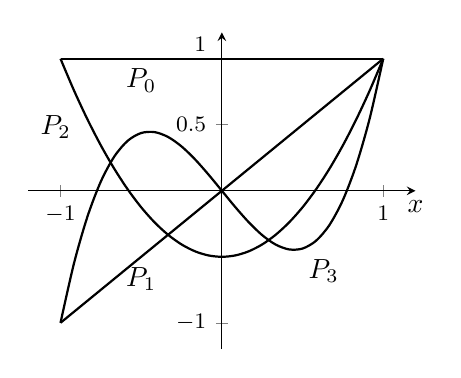
\begin{tikzpicture}[declare function={p0(\x)=1;p1(\x)=\x;p2(\x)=1/2*(3*\x^2-1);p3(\x)=1/2*(5*\x^3-3*\x);}]
\begin{axis}[small,axis lines=middle,xlabel={$x$},ylabel={}, xtick={-1,1},
 xticklabels={$-1$,$1$}, ytick={-1,0.5,1},yticklabels={$-1$,$0.5$,\raisebox{1.25em}{$1$}}, ylabel style={at={(current axis.above origin)},anchor=east},xlabel style={at={(current axis.right of origin)},anchor=north},enlargelimits]
 \addplot[thick,domain=-1:1]{p0(x)}node[pos=0.25,below]{$P_0$};
  \addplot[thick,domain=-1:1]{p1(x)}node[pos=0.25,below]{$P_1$};
   \addplot[thick,domain=-1:1,smooth]{p2(x)}node[pos=0.1,below left]{$P_2$};
    \addplot[thick,domain=-1:1,smooth]{p3(x)}node[pos=0.65,below right]{$P_3$};
 \end{axis}
\end{tikzpicture}
\caption{}
\end{subtable}
\end{table}
جدول \حوالہ{جدول_ابعاد_لیژانڈر_چند_ابتدائی} میں ابتدائی چند لیژانڈر کثیر رکنیاں پیش کی گئی ہیں۔ جیسا کہ نام سے  ظاہر ہے، \عددی{P_{l}(x)} متغیر \عددی{x} کی درجہ \عددی{l} کثیر رکنی ہے، اور \عددی{l} کی قیمت طے  کرتی ہے کہ آیا یہ جفت یا طاق ہو گی۔ تاہم  \عددی{P_{l}^{m}(x)}  عموماً کثیر رکنی نہیں ہو گا؛ اور طاق \عددی{m} کی صورت میں اس میں \عددی{\sqrt{1-x^2}} کا جزو ضربی پایا جائے گا:
\begin{align*}
P_{2}^{0}(x)&=\frac{1}{2}(3x^{2}-1), \quad P_{2}^{1}(x)=(1-x^{2})^{1/2}\frac{\dif}{\dif{x}}\big[\frac{1}{2}(3x^{2}-1)\big]=3x\sqrt{1-x^{2}}, \\
P_{2}^{2}(x)&=(1-x^{2})\big(\frac{\dif}{\dif{x}}\big)^{2}\big[\frac{1}{2}(3x^{2}-1)\big]=3(1-x^{2}),
\end{align*}
وغیرہ وغیرہ۔  (اب ہمیں \عددی{P_{l}^{m}(\cos\theta)} چاہیے اور چونکہ \عددی{\sqrt{1-\cos^{2}\theta}=\sin\theta} ہوتا ہے لہٰذا \عددی{P_{l}^{m}(\cos\theta)} ہر صورت \عددی{\cos\theta} کا کثیر رکنی ہو گا جسے طاق \عددی{m} کی صورت میں
 \عددی{\sin\theta} ضرب کرے گا۔ جدول \حوالہ{جدول_ابعادی_شریک_لیژانڈر_تفاعلات} میں \عددی{\cos\theta} کے چند شریک لیژانڈر تفاعلات پیش کیے گئے ہیں۔)
\begin{table}
\caption{
چند شریک لیژانڈر تفاعلات \عددی{P_l^m(\cos\theta)}: (ا) تفاعلی روپ، (ب) ترسیمات برائے \عددی{r=P_l^m(\cos\theta)} (ان ترسیمات میں \عددی{r} آپ کو \عددی{\theta} رخ تفاعل کی  کل مقدار دیتا ہے؛  ان اشکال کو \عددی{z} محور کے گرد گھمائیں۔)
}
\label{جدول_ابعادی_شریک_لیژانڈر_تفاعلات}
\begin{subtable}{0.60\textwidth}
\centering
\begin{tabular}{ll}
$P_0^0=1$ & $P_2^0=\frac{1}{2}(3\cos^2\theta-1)$\\[0.25em]
$P_1^1=\sin\theta$ & $P_3^3=15\sin\theta(1-\cos^2\theta)$\\[0.25em]
$P_1^0=\cos\theta$ & $P_3^2=15\sin^2\theta\cos\theta$\\[0.25em]
$P_2^2=3\sin^2\theta$ & $P_3^1=\frac{3}{2}\sin\theta(5\cos^2\theta-1)$\\[0.25em]
$P_2^1=3\sin\theta\cos\theta$ & $P_3^0=\frac{1}{2}(5\cos^3\theta-3\cos\theta)$
\end{tabular}
\caption{}
\end{subtable}\hfill
\begin{subtable}{0.35\textwidth}
\centering
\begin{minipage}{0.45\textwidth}
\centering
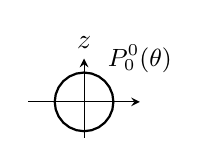
\begin{tikzpicture}[declare function={p00(\x)=1;p11(\x)=sin(90-\x); p10(\x)=cos(90-\x); p21(\x)=3*sin(90-\x)*cos(90-\x); p20(\x)=1/2*(3*cos(90-\x)^2-1); p22(\x)=3*sin(90-\x)^2;}]
\begin{axis}[clip=false,data cs=polar,axis equal,width=3cm,axis lines=middle,xlabel={},ylabel={$z$}, xtick={\empty},  xticklabels={}, ytick={\empty},yticklabels={}, ylabel style={at={(current axis.above origin)},anchor=south},xlabel style={at={(current axis.right of origin)},anchor=west},enlargelimits,ymax=1.25]
 \addplot[thick,domain=0:360]{p00(x)};
 \node[] at (rel axis cs:1,1) {\small{$P_0^0(\theta)$}};
 \end{axis}
\end{tikzpicture}
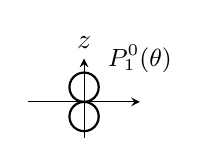
\begin{tikzpicture}[declare function={p00(\x)=1;p11(\x)=sin(90-\x); p10(\x)=cos(90-\x); p21(\x)=3*sin(90-\x)*cos(90-\x); p20(\x)=1/2*(3*cos(90-\x)^2-1); p22(\x)=3*sin(90-\x)^2;}]
\begin{axis}[clip=false,data cs=polar,axis equal,width=3cm,axis lines=middle,xlabel={},ylabel={$z$}, xtick={\empty},  xticklabels={}, ytick={\empty},yticklabels={}, ylabel style={at={(current axis.above origin)},anchor=south},xlabel style={at={(current axis.right of origin)},anchor=west},enlargelimits,ymax=1.25]
   \addplot[thick,domain=0:180,smooth]{p10(x)};
      \addplot[thick,domain=0:180,smooth]{-p10(x)};
       \node[] at (rel axis cs:1,1) {\small{$P_1^0(\theta)$}};
 \end{axis}
\end{tikzpicture}
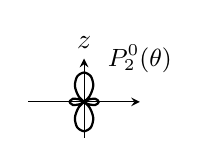
\begin{tikzpicture}[declare function={p00(\x)=1;p11(\x)=sin(90-\x); p10(\x)=cos(90-\x); p21(\x)=3*sin(90-\x)*cos(90-\x); p20(\x)=1/2*(3*cos(90-\x)^2-1); p22(\x)=3*sin(90-\x)^2;}]
\begin{axis}[clip=false,data cs=polar,axis equal,width=3cm,axis lines=middle,xlabel={},ylabel={$z$}, xtick={\empty},  xticklabels={}, ytick={\empty},yticklabels={}, ylabel style={at={(current axis.above origin)},anchor=south},xlabel style={at={(current axis.right of origin)},anchor=west},enlargelimits,ymax=1.25]
    \addplot[thick,domain=0:360,smooth]{p20(x)};
     \node[] at (rel axis cs:1,1) {\small{$P_2^0(\theta)$}};
 \end{axis}
\end{tikzpicture}
\end{minipage}\hfill
\begin{minipage}{0.45\textwidth}
\centering
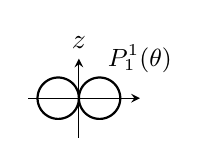
\begin{tikzpicture}[declare function={p00(\x)=1;p11(\x)=sin(90-\x); p10(\x)=cos(90-\x); p21(\x)=3*sin(90-\x)*cos(90-\x); p20(\x)=1/2*(3*cos(90-\x)^2-1); p22(\x)=3*sin(90-\x)^2;}]
\begin{axis}[clip=false,data cs=polar,axis equal,width=3cm,axis lines=middle,xlabel={},ylabel={$z$}, xtick={\empty},  xticklabels={}, ytick={\empty},yticklabels={}, ylabel style={at={(current axis.above origin)},anchor=south},xlabel style={at={(current axis.right of origin)},anchor=west},enlargelimits,xmax=1.25]
  \addplot[thick,domain=0:180,samples=100]{p11(x)};
    \addplot[thick,domain=0:180,samples=100]{-p11(x)};
     \node[] at (rel axis cs:1,1) {\small{$P_1^1(\theta)$}};
 \end{axis}
\end{tikzpicture}
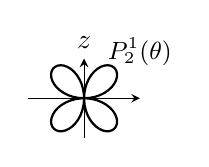
\begin{tikzpicture}[declare function={p00(\x)=1;p11(\x)=sin(90-\x); p10(\x)=cos(90-\x); p21(\x)=3*sin(90-\x)*cos(90-\x); p20(\x)=1/2*(3*cos(90-\x)^2-1); p22(\x)=3*sin(90-\x)^2;}]
\begin{axis}[clip=false,data cs=polar,axis equal,width=3cm,axis lines=middle,xlabel={},ylabel={$z$}, xtick={\empty},  xticklabels={}, ytick={\empty},yticklabels={}, ylabel style={at={(current axis.above origin)},anchor=south},xlabel style={at={(current axis.right of origin)},anchor=west},enlargelimits]
  \addplot[thick,domain=0:360,samples=100]{p21(x)};
   \node[yshift=0.25em] at (rel axis cs:1,1) {\small{$P_2^1(\theta)$}};
 \end{axis}
\end{tikzpicture}
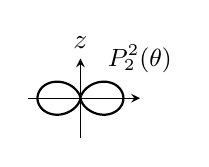
\begin{tikzpicture}[declare function={p00(\x)=1;p11(\x)=sin(90-\x); p10(\x)=cos(90-\x); p21(\x)=3*sin(90-\x)*cos(90-\x); p20(\x)=1/2*(3*cos(90-\x)^2-1); p22(\x)=3*sin(90-\x)^2;}]
\begin{axis}[clip=false,data cs=polar,axis equal,width=3cm,axis lines=middle,xlabel={},ylabel={$z$}, xtick={\empty},  xticklabels={}, ytick={\empty},yticklabels={}, ylabel style={at={(current axis.above origin)},anchor=south},xlabel style={at={(current axis.right of origin)},anchor=west},enlargelimits,xmax=3.5]
  \addplot[thick,domain=0:360,samples=100]{p22(x)};
   \node[] at (rel axis cs:1,1) {\small{$P_2^2(\theta)$}};
 \end{axis}
\end{tikzpicture}
\end{minipage}
\caption{}
\end{subtable}
\end{table}

دھیان رہے کہ صرف غیر منفی عدد صحیح \عددی{l} کی صورت میں کلیہ روڈریگیس معنی خیز ہو گا؛ مزید \عددی{|m|\textgreater{l}} کی صورت میں مساوات \حوالہ{مساوات_ابعادی_شریک_لیژانڈر_تفاعلات_تعریف} کے تحت \عددی{P_{l}^{m}=0} ہو گا۔ یوں \عددی{l} کی کسی بھی مخصوص قیمت کے لئے \عددی{m} کی \عددی{(2l+1)} ممکنہ قیمتیں ہوں گی:
\begin{align}\label{مساوات_ابعادی_انحطاطی_قیمتیں}
l=0,1,2,\dotsc;\quad m=-l,-l+1,\dotsc-1,0,1,\dotsc l-1,l
\end{align}
ذرا رکیے! مساوات  \حوالہ{مساوات_ابعادی_تھیٹا_مساوات} دو رتبی تفرقی مساوات ہے:  \عددی{l} اور \عددی{m} کی کسی بھی قیمتوں کے لئے اس کے  دو خطی غیر تابع حل ہونگے۔ باقی حل کہاں ہیں؟ \ترچھا{جواب:} یقیناً  تفرقی مساوات کے ریاضی حلوں کی  صورت میں باقی حل ضرور موجود ہوں گے،  تاہم  \عددی{\theta=0} اور (یا) \عددی{\theta=\pi} پر ایسے حل بے قابو بڑھتے ہیں (سوال \حوالہ{سوال_ابعادی_طبیعی_نا_قابل_قبول} دیکھیں ) جس کی بنا پر   یہ طبیعی طور  پر ناقابل قبول ہوں گے۔ 

کروی محدد میں حجمی  رکن درج ذیل ہو گا
\begin{align}
\dif^{\,3}\kvec{r}=r^{2}\sin\theta\dif r\dif \theta\dif \phi
\end{align}
لہٰذا معمول زنی شرط (مساوات \حوالہ{مساوات_ابعادی_معمول_زنی_شرط}) درج ذیل روپ اختیار کرتی ہے۔
\begin{align*}
\int\abs{\psi}^{2}r^{2}\sin\theta\dif r \dif\theta\dif\phi=\int\abs{R}^{2}r^{2}\dif r\int\abs{Y}^{2}\sin\theta\dif\theta\dif\phi=1 
\end{align*}
یہاں \عددی{R} اور \عددی{Y} کو علیحدہ علیحدہ  معمول پر لانا زیادہ آسان ثابت ہوتا ہے۔
\begin{align}\label{مساوات_ابعاد_علیحدہ_معمول_زنی_شرائط}
\int_{0}^{\infty}\abs{R}^{2}r^{2}\dif r=1\quad{\text{اور}}\quad \int_{0}^{2\pi}\int_{0}^{\pi}\abs{Y}^{2}\sin\theta\dif \theta\dif \phi=1 
\end{align}
معمول شدہ  زاویائی موجی تفاعلات\حاشیہد{معمول زنی مستقل کو سوال  \حوالہ{سوال_تین_ابعادی_کروی_ہارمونیات_معمول_زنی}  میں حاصل کیا گیا ہے؛  نظریہ زاویائی معیار حرکت میں مستعمل علامتیت کے ساتھ  ہم آہنگی کی خاطر \عددی{\epsilon} (جس کی قیمت \عددی{1} یا \عددی{-1} ہو گی) کی علامت کا انتخاب کیا گیا ہے۔ دھیان رہے کہ \عددی{Y_l^{-m}=(-1)^m(Y_l^m)^*} ہو گا۔} کو \اصطلاح{کروی ہارمونیات}\فرہنگ{کروی!ہارمونیات}\حاشیہب{spherical harmonics}\فرہنگ{spherical!harmonics} کہتے ہیں :
\begin{align}\label{مساوات_ابعادی_کروی_ہارمونیات}
Y_{l}^{m}(\theta,\phi)=\epsilon\sqrt{\frac{(2l+1)}{4\pi}\frac{(l-\abs{m})!}{(l+\abs{m})!}}e^{i{m\phi}}P_{l}^{m}(\cos\theta 
\end{align}
جہاں \عددی{m\geq0} کے لئے \عددی{\epsilon=(-1)^{m}}  اور \عددی{m\leq0}  کے لئے \عددی{\epsilon=1} ہو گا۔ جیسا کہ ہم بعد میں ثابت کریں گے، کروی ہارمونیات عمودی ہیں لہٰذا درج ذیل ہو گا۔
\begin{align}\label{مساوات_ابعادی_کروی_ہارمونی_عمودیت}
\int_{0}^{2\pi}\int_{0}^{\pi}[Y_{l}^{m}(\theta,\phi)]^*[Y_{l'}^{m'}(\theta,\phi)]\sin\theta\dif\theta\dif\phi=\delta_{ll'}\delta_{mm'} 
\end{align}
 جدول \حوالہ{جدول_ابعادی_کروی_ہارمونیات} میں چند ابتدائی  کروی ہارمونیات پیش کیے گئے ہیں۔ تاریخی وجوہات کی بنا پر \عددی{l} کو \اصطلاح{اسّمتی کوانٹائی عدد}\فرہنگ{کوانٹائی عدد!اسّمتی}\حاشیہب{azimuthal quantum number}\فرہنگ{quantum number!azimuthal} جب کہ \عددی{m} کو \اصطلاح{مقناطیسی کوانٹائی عدد}\فرہنگ{کوانٹائی عدد!مقناطیسی}\حاشیہب{magnetic quantum number}\فرہنگ{quantum number!magnetic} کہتے ہیں۔
\begin{table}
\caption{ابتدائی چند کروی ہارمونیات، \عددی{Y_l^m(\theta,\phi)}}
\label{جدول_ابعادی_کروی_ہارمونیات}
\renewcommand{\arraystretch}{2} 
\centering
\begin{tabular}{ll}
$Y_0^0=(\frac{1}{4\pi})^{1/2}$ & $Y_2^{\pm 2}=(\frac{15}{32\pi})^{1/2}\sin^2\theta e^{\pm 2 i \phi}$\\
$Y_1^0=(\frac{3}{4\pi})^{1/2}\cos\theta$ & $Y_3^0=(\frac{7}{16\pi})^{1/2}(5\cos^3\theta-3\cos\theta)$\\
$Y_1^{\pm 1}=\mp(\frac{3}{8\pi})^{1/2}\sin\theta e^{\pm i\phi}$ & $Y_3^{\pm 1}=\mp(\frac{21}{64\pi})^{1/2}\sin\theta(5\cos^2\theta-1)e^{\pm i\phi}$\\
$Y_2^0=(\frac{5}{16\pi})^{1/2}(3\cos^2\theta-1)$ & $Y_3^{\pm 2}=(\frac{105}{32\pi})^{1/2}\sin^2\theta\cos\theta e^{\pm 2 i \phi}$\\
$Y_2^{\pm 1}=\mp(\frac{15}{8\pi})^{1/2}\sin\theta\cos\theta e^{\pm i\phi}$ & $Y_3^{\pm3}=\mp(\frac{35}{64\pi})^{1/2}\sin^3\theta e^{\pm 3 i \phi}$
\end{tabular}
\end{table}
\ابتدا{سوال}\شناخت{سوال_تین_ابعادی_وائے_دو_ایک}
مساوات \حوالہ{مساوات_ابعادی_شریک_لیژانڈر_تفاعلات_تعریف}، \حوالہ{مساوات_ابعادی_روڈریگیس} اور \حوالہ{مساوات_ابعادی_کروی_ہارمونیات} استعمال 
کر کے \عددی{Y_{0}^{0}} اور \عددی{Y_{2}^{1}} تیار کریں۔ تصدیق کریں کہ یہ معمول شدہ اور عمودی ہیں۔
\انتہا{سوال}
%
\ابتدا{سوال}\شناخت{سوال_ابعادی_طبیعی_نا_قابل_قبول}
دکھائیں کہ \عددی{l=m=0} کے لئے
\begin{align*}
\Theta(\theta)=A\ln[\tan(\theta/2)] 
\end{align*}
 مساوات \عددی{\theta} (مساوات \حوالہ{مساوات_ابعادی_تھیٹا_مساوات}) کو مطمئن کرتی ہے۔یہ (وہ) ناقابل قبول دوسرا حل ہے؛ اس میں کیا خرابی ہے؟
\انتہا{سوال}
%
\ابتدا{سوال}\شناخت{سوال_تین_ابعادی_مستقل_معمول_زنی}
مساوات \حوالہ{مساوات_ابعادی_کروی_ہارمونیات} استعمال کر کے \عددی{Y_{l}^{l}(\theta,\phi)} اور 
\عددی{Y_{3}^{2}(\theta,\phi)} مرتب کریں۔(آپ \عددی{P_{3}^{2}} کو  جدول \حوالہ{جدول_ابعادی_شریک_لیژانڈر_تفاعلات} سے دیکھ سکتے ہیں، جبکہ \عددی{P_{l}^{l}} آپ کو مساوات \حوالہ{مساوات_ابعادی_شریک_لیژانڈر_تفاعلات_تعریف} اور \حوالہ{مساوات_ابعادی_روڈریگیس} کی مدد سے  مرتب کرنا  ہو گا۔) تصدیق کیجیے کہ  \عددی{l} اور \عددی{m} کی موزوں قیمتوں کیلئے یہ زاویائی مساوات (مساوات \حوالہ{مساوات_ابعادی_زاویائی_مساوات}) کو  مطمئن کرتے ہیں۔
\انتہا{سوال}
%
\ابتدا{سوال}
کلیہ روڈریگیس سے ابتدا کر کے  لیژانڈر  کثیر رکنیوں کی معیاری عمودیت کی شرط:
\begin{align}
\int_{-1}^{1}P_{l}(x)P_{l'}(x)\dif x=\big(\frac{2}{2l+1}\big)\delta_{ll'} 
\end{align}
اخذ کریں۔ (\ترچھا{اشارہ:} تکمل بالحصص استعمال کریں۔)
\انتہا{سوال}


\جزوحصہ{رداسی مساوات}
دھیان رہے کہ تمام کروی تشاکلی  مخفیہ کے لئے تفاعل موج کا زاویائی حصہ، \عددی{Y(\theta,\phi)}،  ایک  دوسرے جیسا ہو گا؛ مخفیے   \عددی{V(r)} کی شکل و صورت تفاعل موج کے صرف رداسی حصہ، \عددی{R(r)}، پر اثر انداز ہو گی جسے مساوات \حوالہ{مساوات_ابعاد_رداسی_الف} تعین کرتی ہے۔
\begin{align}
\frac{\dif}{\dif r}\big(r^{2}\frac{\dif R}{\dif r}\big)-\frac{2mr^{2}}{\hslash^{2}}[V(r)-E]R=l(l+1)R
\end{align}
نئے متغیرات استعمال کرتے ہوئے اس مساوات کی سادہ روپ حاصل کی جا سکتی ہے: درج ذیل لینے سے
\begin{align}\label{مساوات_ابعادی_نئے_متغیر_رداسی}
u(r)\equiv{rR(r)} 
\end{align}  
\عددی{R=u/r}، \عددی{\dif R/\dif r=[r(\dif u/\dif r)-u]/r^{2}}، \عددی{(\dif /\dif r)[r^{2}(\dif R/\dif r)]=r\dif^{\,2}u/\dif r^{2}}  لہٰذا درج ذیل ہو گا۔
\begin{align}\label{مساوات_ابعادی_رداسی}
-\frac{\hslash^{2}}{2m}\frac{\dif^{\,2}u}{\dif r^{2}}+\big[V+\frac{\hslash^{2}}{2m}\frac{l(l+1)}{r^{2}}\big]u=Eu
\end{align}
اس کو \اصطلاح{رداسی مساوات}\فرہنگ{رداسی مساوات}\حاشیہب{radial equation}\فرہنگ{radial equation} کہتے ہیں\حاشیہد{یہاں \عددی{m} کمیت کو ظاہر کرتی ہے؛ رداسی مساوات میں علیحدگی مستقل \عددی{m} نہیں پایا جاتا ہے۔} جو شکل و صورت کے لحاظ سے یک بعدی مساوات شروڈنگر (مساوات \حوالہ{مساوات_شروڈنگر_علیحدہ_دوم}) کی طرح ہے، تاہم یہاں \اصطلاح{موثر مخفیہ}\فرہنگ{مخفیہ!موثر}\حاشیہب{effective potential}\فرہنگ{potential!effective} درج ذیل ہے
\begin{align}
V_{\text{موثر}}=V+\frac{\hslash^{2}}{2m}\frac{l(l+1)}{r^{2}} 
\end{align}
 جس میں \عددی{(\hslash^{2}/2m)[l(l+1)/r^{2}]}  اضافی جزو پایا جاتا ہے جو \اصطلاح{مرکز گریز جزو}\فرہنگ{مرکز گریز جزو}\حاشیہب{centrifugal term}\فرہنگ{centrifugal term} کہلاتا ہے۔ یہ کلاسیکی میکانیات کے مرکز گریز (مجازی) قوت کی طرح، ذرہ کو (مبدا سے دور) باہر جانب دھکیلتا ہے۔ یہاں معمول زنی شرط (مساوات \حوالہ{مساوات_ابعاد_علیحدہ_معمول_زنی_شرائط}) درج ذیل روپ اختیار کرتی ہے۔ 
\begin{align}
\int_{0}^{\infty}\abs{u}^{2}\dif r=1 
\end{align}
کسی مخصوص مخفیہ \عددی{V(r)}   کے بغیر ہم آگے نہیں بڑھ سکتے۔
%==================

\ابتدا{مثال}
درج ذیل  \اصطلاح{لامتناہی کروی کنویں}\فرہنگ{لامتناہی کروی کنواں}\حاشیہب{infinite spherical well}\فرہنگ{infinite spherical well}   پر غور کریں۔
\begin{align}
V(r)=\begin{cases}
0&r\le {a}\\
\infty&r>a
\end{cases} 
\end{align}
اس کے تفاعلات موج اور اجازتی توانائیاں تلاش کریں۔

\ترچھا{حل:}\quad
کنویں  کے باہر تفاعل موج صفر ہے جب کے کنویں  کے اندر رداسی مساوات درج ذیل ہے
\begin{align}\label{مساوات_ابعادی_مربعی_کنواں_الف}
\frac{\dif^{\,2}u}{\dif r^{2}}=\big[\frac{l(l+1)}{r^{2}}-k^{2}\big]u 
\end{align}
جہاں ہمیشہ کی طرح درج ذیل ہو گا۔
\begin{align}
k\equiv\frac{\sqrt{2mE}}{\hslash} 
\end{align}
ہم نے اس مساوات کو، سرحدی شرط \عددی{u(a)=0} مسلط کر کے، حل کرنا ہے۔ سب سے آسان صورت \عددی{l= 0} کی ہے۔
\begin{align*}
\frac{\dif^{\,2}u}{\dif r^{2}}=-k^{2}u\implies {u(r)=A\sin(kr)+B\cos(kr)} 
\end{align*}
یاد رہے،  اصل رداسی تفاعل موج \عددی{R(r)=u(r)/r} ہے اور \عددی{r\to{0}}  کی صورت میں \عددی{[\cos(kr)]/r}  بے قابو بڑھتا ہے۔یوں ہمیں \عددی{B=0} منتخب\حاشیہد{درحقیقت ہم صرف اتنا چاہتے ہیں کہ تفاعل موج معمول پر لانے کے قابل ہو؛ یہ ضروری نہیں کہ یہ متناہی ہو: مساوات \حوالہ{مساوات_ابعاد_علیحدہ_معمول_زنی_شرائط} میں \عددی{r^2} کی بنا پر مبدا پر \عددی{R(r)\sim 1/r} معمول پر لانے کے قابل ہے۔} کرنا ہو گا۔ اب سرحدی شرط پر پورا اترنے کے لئے ضروری ہے  کہ \عددی{\sin(ka)=0} ہو لہٰذا   \عددی{ka=n\pi} ہو گا جہاں \عددی{n}  عدد صحیح ہے۔ ظاہر ہے کہ اجازتی توانائیاں درج ذیل ہوں گی
\begin{align}
E_{n0}&=\frac{n^{2}\pi^{2}\hslash^{2}}{2ma^{2}},&&(n=1,2,3,...). 
\end{align}
جو عین یک بعدی لامتناہی چکور کنویں  کی توانائیاں ہیں (مساوات \حوالہ{مساوات_شروڈنگر_لامتناہی_چکور_کنواں_توانائیاں})۔ \عددی{u(r)}  کو معمول پر لانے سے \عددی{A=\sqrt{2/a}} حاصل ہو گا۔ زاویائی جزو (جو \عددی{Y_{0}^{0}(\theta,\phi)=1/\sqrt{4\pi}}  ہے لہٰذا اس کی شمولیت یہاں ایک حقیر سا کام ہے) کو ساتھ منسلک کرتے ہوئے درج ذیل حاصل ہو گا۔ 
\begin{align}
\psi_{n00}=\frac{1}{\sqrt{2\pi a}}\frac{\sin(n\pi r/a)}{r} 
\end{align}
[دھیان کیجیے کہ ساکن حالات کے نام تین \اصطلاح{کوانٹائی اعداد}\فرہنگ{کوانٹائی اعداد}\حاشیہب{quantum numbers}\فرہنگ{quantum numbers} \عددی{n}، \عددی{l} اور \عددی{m} استعمال کر کے رکھے جاتے ہیں: \عددی{\psi_{nml}(r,\theta,\phi)}؛ جبکہ توانائی، \عددی{E_{nl}}،   صرف \عددی{n} اور \عددی{l} پر منحصر ہو گی۔] 

(ایک اختیاری عدد صحیح \عددی{l} کے لئے) مساوات \حوالہ{مساوات_ابعادی_مربعی_کنواں_الف} کا عمومی حل
\begin{align}
u(r)=Arj_{l}(kr)+Brn_{l}(kr). 
\end{align}
 بہت جانا پہچانا نہیں ہے  جہاں \عددی{j_{l}(x)} رتبہ \عددی{l} کا  \اصطلاح{کروی بیسل تفاعل}\فرہنگ{بیسل!کروی تفاعل}\حاشیہب{spherical Bessel function}\فرہنگ{Bessel!spherical function} ہے اور \عددی{n_{l}(x)} رتبہ \عددی{l} کا  \اصطلاح{کروی نیومن تفاعل}\فرہنگ{نیومن!کروی تفاعل}\حاشیہب{spherical Neumann function}\فرہنگ{Neumann!spherical function}  ہے جن کی تعریفات درج ذیل ہیں۔  
\begin{align}\label{مساوات_ابعادی_تعریفات_کروی_بیسل_نیومن}
j_{l}(x)\equiv(-x)^{l}\big(\frac{1}{x}\frac{\dif}{\dif x}\big)^{l}\frac{\sin x}{x};\quad n_{l}(x)\equiv-(-x)^{l}
\big(\frac{1}{x}\frac{\dif}{\dif x}\big)^{l}\frac{\cos x}{x}
\end{align}
مثال کے طور پر درج ذیل ہوں گے، وغیرہ وغیرہ۔
\begin{align*}
j_{0}(x)&=\frac{\sin x}{x};\quad n_{0}(x)=-\frac{\cos x}{x};\\
j_1(x)&=(-x)\frac{1}{x}\frac{\dif}{\dif x}\big(\frac{\sin x}{x}\big)=\frac{\sin x}{x^{2}}-\frac{\cos x}{x};\\
j_{2}(x)&=(-x)^{2}\big(\frac{1}{x}\frac{\dif}{\dif x}\big)^{2}\frac{\sin x}{x}=x^{2}\big(\frac{1}{x}\frac{\dif}{\dif x}\big)\frac{x\cos x-\sin x}{x^{3}}\\
&=\frac{3\sin x-3x\cos x-x^2\sin x}{x^{3}}
\end{align*}
\begin{table}
\caption{
ابتدائی چند کروی بیسل اور نیومن تفاعلات، \عددی{j_n(x)} اور \عددی{n_l(x)}؛ چھوٹی \عددی{x} کے لئے متقاربی روپ۔
}
\label{جدول_ابعادی_کروی_بیسل_نیومن_تفاعلات}
\centering
\renewcommand{\arraystretch}{2} 
\begin{tabular}{ll}
\toprule
$j_0=\frac{\sin x}{x}$  &  $n_0=-\frac{\cos x}{x}$\\
$j_1=\frac{\sin x}{x^2}-\frac{\cos x}{x}$  &  $n_1=-\frac{\cos x}{x^2}-\frac{\sin x}{x}$\\
$j_2=\big(\frac{3}{x^3}-\frac{1}{x}\big)\sin x-\frac{3}{x^2}\cos x$  &  $n_2=-\big(\frac{3}{x^3}-\frac{1}{x}\big)\cos x-\frac{3}{x^2}\sin x$\\[0.5em]
\midrule
$j_l\to\frac{2^l l!}{(2l+1)!}x^l$  &  $n_l\to -\frac{(2l)!}{2^ll!}\frac{1}{x^{l+1}},\quad x\ll 1$\\
\bottomrule
\end{tabular}
\end{table}
جدول \حوالہ{جدول_ابعادی_کروی_بیسل_نیومن_تفاعلات} میں ابتدائی چند کروی بیسل اور نیومن تفاعلات پیش کیے گئے ہیں۔ متغیر \عددی{x} کی چھوٹی قیمت کے لئے جہاں
\begin{align*}
\sin x\approx x-\frac{x^{3}}{3!}+\frac{x^{5}}{5!}-\dotsb\quad \text{اور}\quad  \cos x \approx 1-\frac{x^{2}}{2!}+\frac{x^{4}}{4!}-\dotsb
\end{align*}
 ہوں گے، درج ذیل ہوں گے، وغیرہ وغیرہ۔
\begin{align*}
j_{0}(x)\approx1;\quad{n_{0}(x)\approx-\frac{1}{x}};\quad{j_{1}(x)\approx\frac{x}{3}};\quad{j_{2}(x)\approx\frac{x^{2}}{15}}; 
\end{align*}
 دھیان رہے کہ مبدا  پر بیسل تفاعلات متناہی  ہیں جبکہ مبدا پر نیومن تفاعلات بے قابو بڑھتے ہیں۔ یوں ہمیں لازماً  \عددی{B_{l}=0} منتخب کرنا ہو گا لہٰذا درج ذیل ہو گا۔
\begin{align}
R(r)=Aj_{l}(kr) 
\end{align}
اب سرحدی شرط \عددی{R(a)=0} کو مطمئن کرنا باقی ہے۔ ظاہر ہے کہ \عددی{k} کو درج ذیل کے تحت منتخب کرنا ہو گا
\begin{align}
j_{l}(ka)=0
\end{align}
یعنی \عددی{l} رتبی کروی بیسل تفاعل کا \عددی{(ka)} ایک صفر ہو گا۔ اب بیسل تفاعلات ارتعاشی ہیں (شکل \حوالہ{شکل_تین_ابعادی_چار_کروی_بیسل_تفاعلات}  دیکھیں)؛ ہر ایک کے لامتناہی تعداد  صفر پائے جاتے ہیں۔
%fig 4.2 p155
\begin{figure}
\centering
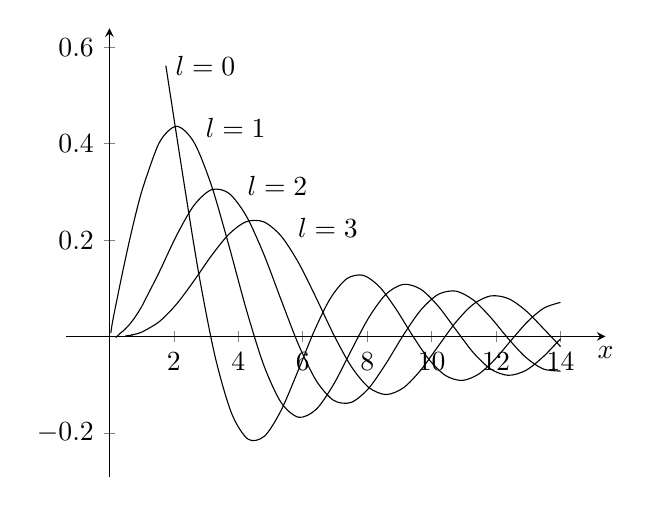
\begin{tikzpicture}[declare function={j0(\x)=sin(deg(\x))/\x;j1(\x)=sin(deg(\x))/\x^2-cos(deg(\x))/\x; 
j2(\x)=3/\x*j1(\x)-j0(\x);j3(\x)=5/\x*j2(\x)-j1(\x);}]
\begin{axis}[axis lines=middle,xlabel={$x$},ylabel={}, xtick={2,4,6,8,10,12,14},ylabel style={at={(current axis.above origin)},anchor=east},xlabel style={at={(current axis.right of origin)},anchor=north},enlargelimits]
\addplot[domain=1.75:14,smooth]{j0(x)}node[pos=0,right]{$l=0$};
\addplot[domain=1:14,smooth]{j1(x)}node[pos=0.13,above right]{$l=1$};
\addplot[domain=0:1,smooth]{j1(x)};
\addplot[domain=1:14,smooth]{j2(x)}node[pos=0.23,above right]{$l=2$};
\addplot[domain=0.2:1,smooth]{j2(x)};
\addplot[domain=1:14,smooth]{j3(x)}node[pos=0.35,above right]{$l=3$};
\addplot[domain=0.5:1,smooth]{j3(x)};
\end{axis}
\end{tikzpicture}
\caption{ابتدائی چار کروی بیسل تفاعلات۔}
\label{شکل_تین_ابعادی_چار_کروی_بیسل_تفاعلات}
\end{figure}




 تاہم (ہماری بدقسمتی سے) یہ ایک جیسے فاصلوں پر نہیں پائے جاتے  (جیسا کہ نقاط \عددی{n} یا نقاط \عددی{n\pi}، وغیرہ پر)؛ انہیں اعدادی تراکیب سے حاصل کرنا ہو گا۔ بہرحال سرحدی شرط کے تحت درج ذیل ہو گا
\begin{align}
k=\frac{1}{a}\beta_{nl} 
\end{align}
جہاں \عددی{\beta_{nl}} رتبہ  \عددی{l}   کروی بیسل تفاعل کا \عددی{n} واں صفر   ہو گا۔ یوں اجازتی توانائیاں 
\begin{align}\label{مساوات_ابعاد_کروی_کنواں_اجازتی_توانائیاں}
E_{nl}=\frac{\hslash^{2}}{2ma^{2}}\beta_{nl}^{2}. 
\end{align}
اور تفاعلات موج درج ذیل ہوں گے 
\begin{align}
\psi_{nlm}(r,\theta,\phi)=A_{nl}j_{l}(\beta_{nl}r/a)Y_{l}^{m}(\theta,\phi). 
\end{align}
جہاں مستقل \عددی{A_{n1}} کا تعین معمول زنی سے کیا جاتا ہے۔چونکہ \عددی{l} کی ہر ایک قیمت کے لئے \عددی{m} کی \عددی{(2l+1)}
مختلف قیمتیں پائی جاتی ہیں لہٰذا توانائی کی ہر سطح \عددی{(2l+1)} گنّا انحطاطی ہو گی (مساوات \حوالہ{مساوات_ابعادی_انحطاطی_قیمتیں} دیکھیں)۔
\انتہا{مثال}
%===============
\ابتدا{سوال}
\begin{enumerate}[a.]
\item
کروی نیومن تفاعلات \عددی{n_{1}(x)} اور \عددی{n_{2}(x)} کو (مساوات \حوالہ{مساوات_ابعادی_تعریفات_کروی_بیسل_نیومن}) میں پیش کی گئی تعریفات سے)  تیار کریں۔
\item
سائن اور کوسائن کو پھیلا کر \عددی{x\ll1} کے لئے كارآمد  \عددی{n_{1}(x)} اور \عددی{n_{2}(x)} کے  تخمینی کلیات  اخذ کریں۔تصدیق کریں کہ یہ مبدا پر بےقابو بڑھتے ہیں۔
\end{enumerate}
\انتہا{سوال}
%
\ابتدا{سوال}
\begin{enumerate}[a.]
\item
 تصدیق کریں کہ \عددی{V(r)=0} اور \عددی{l=1} کے لئے \عددی{Arj_{l}(kr)} رداسی مساوات کو مطمئن کرتا ہے۔
\item
لامتناہی کروی کنویں  کیلئے \عددی{l=1} کی صورت میں اجازتی توانائیاں ترسیم کی مدد سے تعین کریں۔ دکھائیں کہ \عددی{n} کی بڑی قیمت کے لئے 
\عددی{E_{n1}\approx(\hslash^{2}\pi^{2}/2ma^{2})(n+1/2)^{2}} ہو گا۔(\ترچھا{اشارہ:} پہلے  
\عددی{j_{1}(x)=0\implies {x}=\tan x} دکھائیں۔ اس کے بعد \عددی{x} اور \عددی{\tan x} کو ایک ساتھ ترسیم کرتے ہوئے ان کے نقاط تقاطع تلاش کریں۔)
\end{enumerate}
\انتہا{سوال}
%
\ابتدا{سوال}
 ایک ذرہ جس کی کمیت \عددی{m} ہے کو \ترچھا{متناہی} کروی کنواں:
\begin{align*}
V(r)=\begin{cases}-V_{0}&r\le a\\0&r>a\\\end{cases} 
\end{align*}
میں رکھا جاتا ہے۔ اس کا زمینی حال، \عددی{l=0}  کے لئے،  رداسی مساوات کے حل سے حاصل کریں۔ دکھائیں کہ 
\عددی{V_{0}a^{2}<\pi^{2}\hslash^{2}/8m} کی صورت میں کوئی مقید حال نہیں پایا جائے گا۔
\انتہا{سوال}
%======================
\حصہ{ہائیڈروجن جوہر}\شناخت{حصہ_تین_بعدی_ہائیڈروجن_جوہر}
ہائیڈروجن جوہر بار \عددی{e} کے  ایک بھاری پروٹان جس کے گرد بار \عددی{-e} کا ایک ہلکا الیکٹران طواف کرتا ہو پر مشتمل ہوتا ہے۔ پروٹان بنیادی طور پر ساکن رہتا ہے (جسے ہم مبدا پر تصور کر سکتے ہیں)۔  ان دونوں کے مخالف بار کے بیچ قوت کشش پائی جاتی ہے جو انہیں اکٹھے رکھتی ہے  (شکل \حوالہ{شکل_تین_ابعادی_ہائیڈروجن_جوہر} دیکھیں)۔  قانون کولمب کے تحت مخفی توانائی (بین الاقوامی اکائیوں میں)  درج ذیل ہو گی  
 \begin{align}\label{مساوات_ابعادی_کولمب_مخفیہ}
V(r)=-\frac{e^{2}}{4\pi\epsilon_{0}}\frac{1}{r} 
\end{align}
لہٰذا رداسی مساوات (مساوات  \حوالہ{مساوات_ابعادی_رداسی})  درج ذیل روپ اختیار کرے گی۔
\begin{align}\label{مساوات_ابعادی_رداسی_کولمب}
-\frac{\hslash^{2}}{2m}\frac{\dif^{\,2}{u}}{\dif r^{2}}+\big[-\frac{e^{2}}{4\pi\epsilon_{0}}\frac{1}{r}+\frac{\hslash^{2}}{2m}\frac{l(l+1)}{r^{2}}\big]u=Eu 
\end{align}

%fig 4.3

\begin{figure}
\centering
\begin{tikzpicture}
\pgfmathsetmacro{\r}{1.5}
\pgfmathsetmacro{\ra}{1.5-3/72}
\pgfmathsetmacro{\ang}{30}
\draw (0,0) circle (\r);
\draw[-latex] (0,0) node[circle,fill,inner sep=1.5pt]{} node[left]{$+e$} node[below left]{\RL{(پروٹان)}} -- (\ang:\ra) node[right]{$-e$} node[below right,xshift=0.4em]{\RL{(الیکٹران)}} node[pos=0.5, above]{$r$}node[circle,fill,inner sep=1.5pt]{};
\end{tikzpicture}
\caption{ہائیڈروجن  جوہر}
\label{شکل_تین_ابعادی_ہائیڈروجن_جوہر}
\end{figure}


 ہم نے اس مساوات کو  \عددی{u(r)}   کے لئے حل کر کے اجازتی توانائیاں \عددی{E} تعین کرنی ہیں۔  ہائیڈروجن جوہر کا حل نہایت اہم ہے لہٰذا میں اس کو، ہارمونی مرتعش کے تحلیلی حل کی ترکیب سے، قدم با قدم حل کر کے پیش کرتا ہوں۔ (جس قدم پر آپ کو دشواری پیش آئے، حصہ \حوالہ{حصہ_شروڈنگر_تحلیلی_ترکیب} سے مدد لیں جہاں مکمل تفصیل پیش کی گئی ہے۔)  کولمب مخفیہ،  مساوات \حوالہ{مساوات_ابعادی_کولمب_مخفیہ}،    (\عددی{E>0} کے لئے)  \ترچھا{استمراریہ} حالات، جو الیکٹران پروٹون بکھراو کو ظاہر کرتے ہیں، تسلیم کرنے کے ساتھ ساتھ غیر مسلسل \ترچھا{مقید} حالات، جو ہائیڈروجن جوہر کو ظاہر کرتے ہیں، بھی تسلیم کرتا ہے۔ ہماری دلچسپی موخر الذکر میں ہے۔

\جزوحصہ{رداسی تفاعل موج}
 سب سے پہلے نئی علامتیں متعارف کرتے ہوئے مساوات کی بہتر (صاف) صورت حاصل کرتے ہیں۔ درج ذیل متعارف کر کے (جہاں مقید حالات کے لئے \عددی{e} منفی ہونے کی وجہ سے \عددی{\kappa }  حقیقی ہو گا)
 \begin{align}\label{مساوات_ابعادی_متعارف_الف}
\kappa \equiv \frac{\sqrt{-2mE}}{\hslash} 
\end{align}
 مساوات \حوالہ{مساوات_ابعادی_رداسی_کولمب} کو \عددی{E} سے تقسیم کرنے سے
\begin{align*}
\frac{1}{\kappa ^{2}}\frac{\dif^{\,2}{u}}{\dif{r^{2}}}=\big[1-\frac{me^{2}}{2\pi\epsilon_{0}\hslash^{2}\kappa }\frac{1}{(\kappa r)}+\frac{l(l+1)}{(\kappa r)^{2}}\big]u 
\end{align*}
حاصل ہو گا جس کو دیکھ کر ہمیں خیال آتا ہے کہ ہم درج ذیل علامتیں متعارف کریں 
\begin{align}\label{مساوات_ابعادی_متعارف_ب}
\rho\equiv \kappa r, \quad \rho_{0}\equiv\frac{me^{2}}{2\pi\epsilon_{0}\hslash^{2}\kappa } 
\end{align}
لہٰذا درج ذیل لکھا جائے گا۔
\begin{align}\label{مساوات_ابعادی_رداسی_کولمب_نئے_متغیرات}
\frac{\dif^{\,2}{u}}{\dif{\rho^{2}}}=\big[1-\frac{\rho_{0}}{\rho}+\frac{l(l+1)}{\rho^{2}}\big]u 
\end{align}

اس کے بعد ہم حالات کے  متقاربی روپ پر غور کرتے ہیں۔ اب \عددی{\rho\to\infty} کرنے سے قوسین کے اندر مستقل جزو غالب ہو گا لہٰذا (تخمیناً) درج ذیل لکھا جا سکتا ہے۔
\begin{align*}
\frac{\dif^{\,2}{u}}{\dif{\rho^{2}}}=u 
\end{align*}
اس کا عمومی حال درج ذیل ہے
\begin{align}\label{مساوات_ابعاد_عمومی_حل_بے_قابو}
u(\rho)=Ae^{-\rho}+Be^{\rho} 
\end{align}
تا ہم  (\عددی{\rho\to\infty} کی صورت میں) \عددی{e^{\rho}} بے قابو بڑھتا ہے لہٰذا ہمیں \عددی{B=0} لینا ہو گا۔ یوں \عددی{\rho} کی بڑی قیمتوں کے لیے درج  ذیل ہو گا۔
\begin{align}
u(\rho)\sim Ae^{-\rho} 
\end{align}
اس کے برعکس \عددی{\rho\to 0} کی صورت میں مرکز گریز جزو غالب ہو گا؛\حاشیہد{یہ دلیل \عددی{l=0} کی صورت میں کارآمد نہیں ہو گی (اگرچہ مساوات \حوالہ{مساوات_ابعادی_ہائیڈروجن_مبدا_قریب} میں پیش نتیجہ اس صورت کے لئے بھی درست ہے)۔ بہرحال، میرا مقصد نئی علامتیت (مساوات \حوالہ{مساوات_ابعادی_نئی_علامتیت}) کے استعمال کے لئے راستہ ہموار کرنا ہے۔} لہٰذا تخمیناً  درج ذیل لکھا جا سکتا ہے۔ 
\begin{align*}
\frac{\dif^{\,2}{u}}{\dif{\rho^{2}}}=\frac{l(l+1)}{\rho^{2}}u 
\end{align*}
 جس کا عمومی حل (تصدیق کیجیے) درج ذیل ہو گا
 \begin{align*}
u(\rho)=C\rho^{l+1}+D\rho^{-l} 
\end{align*}
 تاہم  (\عددی{\rho\to0}  کی صورت میں)  \عددی{\rho^{-l}}  بے قابو بڑھتا ہے لہٰذا \عددی{D=0}  ہو گا۔ یوں  \عددی{\rho}  کی چھوٹی قیمتوں کے لیے درج ذیل ہو گا۔
 \begin{align}\label{مساوات_ابعادی_ہائیڈروجن_مبدا_قریب}
u(\rho)\sim C\rho^{l+1} 
\end{align}

  اگلے قدم پر متقاربی رویہ  کو چھیلنے کی خاطر  نیا تفاعل \عددی{v(\rho)}:
  \begin{align}\label{مساوات_ابعادی_نئی_علامتیت}
u(\rho)=\rho^{l+1}e^{-\rho}v(\rho) 
\end{align}
  اس امید سے متعارف کرتے ہیں کہ    \عددی{u(\rho)}     سے  \عددی{v(\rho)} زیادہ سادہ ہو گا۔ ابتدائی نتائج 
\begin{align*}
\frac{\dif u}{\dif \rho}=\rho^l e^{-\rho} \big[(l+1-\rho)v+\rho\frac{\dif v}{\dif \rho}\big]
\end{align*}
اور
\begin{align*}
\frac{\dif^{\,2}u}{\dif \rho^2}=\rho^le^{-\rho}\big\{\big[-2l-2+\rho+\frac{l(l+1)}{\rho}\big]v+2(l+1-\rho)\frac{\dif v}{\dif \rho}+\rho\frac{\dif^{\,2}v}{\dif \rho^2}\big\}
\end{align*}
خوش آئین نظر نہیں آتے ہیں۔   اس طرح \عددی{v(\rho)} کی صورت میں رداسی مساوات (مساوات \حوالہ{مساوات_ابعادی_رداسی_کولمب_نئے_متغیرات})   درج ذیل روپ اختیار کرتی ہے۔
  \begin{align}\label{مساوات_ابعادی_رداسی_نئی_روپ}
\rho\frac{\dif^{\,2}{v}}{\dif{\rho^{2}}}+2(l+1-\rho)\frac{\dif{v}}{\dif{\rho}}+[\rho_{0}-2(l+1)]v=0 
\end{align}

  آخر میں ہم فرض کرتے ہیں کہ حل،   \عددی{v(\rho)}،  کو \عددی{\rho} کا طاقتی تسلسل لکھا جا سکتا ہے۔
  \begin{align}
v(\rho)=\sum_{j=0}^{\infty}c_{j}\rho^{j} 
\end{align}
ہمیں عددی سر (\عددی{c_0}، \عددی{c_1}، \عددی{c_2}، وغیرہ) تلاش کرنے ہوں گے۔  جزو در جزو تفرق لیتے ہیں۔
\begin{align*}
\frac{\dif{v}}{\dif{\rho}}=\sum_{j=0}^{\infty}jc_{j}\rho^{j-1}=\sum_{j=0}^{\infty}(j+1)c_{j+1}\rho^{j} 
\end{align*}
[میں نے دوسرے مجموعہ میں "فرضی اشاریہ" \عددی{j} کو \عددی{j+1} کہا ہے۔ اگر آپکو یقین نہ  ہو تو اولین چند اجزاء صریحاً لکھ کر تصدیق کر لیں۔ آپ سوال اٹھا سکتے ہیں کے نیا مجموعہ \عددی{j=-1}  سے کیوں  شروع نہیں کیا گیا؛ تاہم جزو ضربی \عددی{(j+1)}  اس جزو کو ختم کرتا ہے لہٰذا ہم صفر سے بھی شروع کر سکتے ہیں۔] دوبارہ تفرق لیتے ہیں۔
\begin{align*}
\frac{\dif^{\,2}{v}}{\dif{\rho^{2}}}=\sum_{j=0}^{\infty}j(j+1)c_{j+1}\rho^{j-1} 
\end{align*}
انہیں مساوات \حوالہ{مساوات_ابعادی_رداسی_نئی_روپ} میں پر کرتے ہیں۔
\begin{multline*}
\sum_{j=0}^{\infty}j(j+1)c_{j+1}\rho^{j}+2(l+1)+\sum_{j=0}^{\infty}(j+1)c_{j+1}\rho^{j} \\
-2\sum_{j=0}^{\infty}jc_{j}\rho^{j}+[\rho_{0}-2(l+1)]\sum_{j=0}^{\infty}c_{j}\rho^{j}=0 
\end{multline*}
ایک جیسی طاقتوں کے عددی سروں کو مساوی رکھتے ہوئے
\begin{align*}
j(j+1)c_{j+1}+2(l+1)(j+1)c_{j+1}-2jc_{j}+[\rho_{0}-2(l+1)]c_{j}=0 
\end{align*}
یا
\begin{align}\label{مساوات_ابعادی_کولمب_کلیہ_توالی}
c_{j+1}=\left\{\frac{2(j+l+1)-\rho_{0}}{(j+1)(j+2l+2)}\right\}c_{j} 
\end{align}
ہو گا۔ یہ کلیہ توالی عددی سر تعین کرتے ہوئے تفاعل \عددی{v(\rho)} تعین کرتا ہے۔ ہم \عددی{c_{0}} سے شروع کر کے (جو مجموعی مستقل کا روپ اختیار کرتا ہے جسے آخر میں معمول زنی سے حاصل کیا جائے گا)، مساوات \حوالہ{مساوات_ابعادی_کولمب_کلیہ_توالی}  سے \عددی{c_{1}} تعین کرتے ہیں؛ جس کو واپس اسی مساوات میں پر کر کے \عددی{c_{2}} تعین ہو گا، وغیرہ، وغیرہ۔\حاشیہد{آپ پوچھ سکتے ہیں: طاقتی تسلسل کی ترکیب \عددی{u(\rho)} پر ہی کیوں لاگو نہیں کی گئی؛ اس ترکیب کے اطلاق سے قبل متقاربی رویہ کو کیوں (جزو ضربی کی صورت میں) باہر نکالا گیا؟ درحقیقت اس کی وجہ نتائج کی خوبصورتی ہے۔جزو ضربی \عددی{\rho^{l+1}} باہر نہ نکالنے سے تسلسل کے  ابتدائی اجزاء صفر ہوں گے (پہلا غیر صفر عددی سر \عددی{c_{l+1}} ہو گا)؛ \عددی{\rho^{l+1}}  باہر نکالنے سے تسلسل کا پہلا جزو \عددی{\rho^0} حاصل ہو گا۔ اس کے برعکس جزو ضربی \عددی{e^{-\rho}}  باہر نکالنا زیادہ ضروری ہے؛ اسے باہر نہ نکالنے سے \عددی{c_{j+2}}، \عددی{c_{j+1}} اور \عددی{c_j} پر مشتمل  تین اجزائی کلیہ توالی حاصل ہوتا ہے (کر کے دیکھیں!) جس کے ساتھ کام کرنا زیادہ مشکل ثابت ہوتا ہے۔}

 آئیں \عددی{j} کی بڑی قیمت (جو \عددی{\rho}  کی بڑی قیمت کی مطابقتی ہو گی  جہاں بلند طاقتیں غالب ہوں گی) کے لئے عددی سروں کی صورت دیکھیں ۔ یہاں  کلیہ توالی درج ذیل کہتا ہے۔\حاشیہد{آپ پوچھ سکتے ہیں: شمار کنندہ میں \عددی{2(l+1)-\rho_0} اور نسب نما میں \عددی{2l+2} رد کرنے کی طرح \عددی{j+1} میں \عددی{1} کیوں رد نہیں کیا جاتا؟ اس تخمین میں ایسا کیا جا سکتا ہے، تاہم اسے رد نہ کرنے سے دلیل زیادہ واضح ہو گا۔ آپ \عددی{1} کو رد کر کے دیکھ سکتے ہیں کہ میں کیا کہنا چاہتا ہوں۔}
\begin{align*}
c_{j+1}\cong\frac{2j}{j(j+1)}c_{j}=\frac{2}{j+1}c_{j} 
\end{align*}
ایک لمحہ کے لیے فرض کریں  کہ یہ بالکل ٹھیک ٹھیک رشتہ ہے۔ تب 
\begin{align}
c_{j}=\frac{2^{j}}{j!}c_{0} 
\end{align}
لہٰذا
\begin{align*}
v(\rho)=c_{0}\sum_{j=0}^{\infty}\frac{2^{j}}{j!}\rho^{j}=c_{0}e^{2\rho} 
\end{align*}
 اور یوں  درج ذیل ہو گا
\begin{align}
u(\rho)=c_{0}\rho^{l+1}e^{\rho} 
\end{align}
 جو   \عددی{\rho}  کی بڑی قیمتوں کے لیے  بے قابو بڑھتا ہے۔ مثبت قوت نما وہی غیر پسندیدہ متقاربی رویہ دیتا ہے جو مساوات \حوالہ{مساوات_ابعاد_عمومی_حل_بے_قابو} میں پایا گیا۔ (در حقیقت  متقاربی حل بھی رداسی مساوات کے جائز حل ہیں البتہ ہم ان میں دلچسپی نہیں رکھتے  کیونکہ یہ معمول پر  لانے کے قابل نہیں ہیں۔) اس المیہ سے نجات کا صرف ایک ہی راستہ ہے؛ تسلسل کو کہیں نہ کہیں اختتام پذیر ہونا ہو گا۔ لازمی طور پر ایک ایسا زیادہ سے زیادہ عدد صحیح، \عددی{j_{\text{بلندتر}}}، پایا جائے گا جس پر درج ذیل ہو۔
 \begin{align}
c_{(j_{\text{بلندتر}}+1)}=0
\end{align}
 (یوں کلیہ توالی کے تحت باقی تمام (زیادہ بلند) عددی سر صفر ہوں گے۔)  مساوات \حوالہ{مساوات_ابعادی_کولمب_کلیہ_توالی} سے ظاہر ہے کہ درج ذیل ہو گا۔
 \begin{align*}
2(j_{\text{بلندتر}}+l+1)-\rho_{0}=0 
\end{align*}
\اصطلاح{صدر کوانٹم  عدد}\فرہنگ{کوانٹم!صدر عدد}\حاشیہب{principal quantum number}\فرہنگ{quantum!principle number}
 \begin{align}\label{مساوات_ابعادی_صدر_کوانٹائی_عدد}
n\equiv j_{\text{بلندتر}}+l+1 
\end{align}
 متعارف کرتے ہوئے درج ذیل ہو گا۔
 \begin{align}\label{مساوات_ابعادی_رو_این}
\rho_{0}=2n 
\end{align}
 اب \عددی{E} کو  \عددی{\rho_{0}}  تعین کرتا ہے (مساوات \حوالہ{مساوات_ابعادی_متعارف_الف} اور \حوالہ{مساوات_ابعادی_متعارف_ب})
 \begin{align}
E=-\frac{\hslash^{2}\kappa ^{2}}{2m}=-\frac{me^{4}}{8\pi^{2}\epsilon^{2}\hslash^{2}\rho^{2}} 
\end{align}
 لہٰذا اجازتی توانائیاں درج ذیل ہوں گی۔ 
 \begin{align}\label{مساوات_ابعادی_ہائیڈروجن_اجازتی_توانائیاں}
E_{n}&=-\big[\frac{m}{2\hslash^{2}}\big(\frac{e^{2}}{4\pi\epsilon}\big)^{2}\big]\frac{1}{n^{2}}=\frac{E_{1}}{n^{2}}, && n=1,2,3,\dotsc
\end{align}
 یہ مشہور  زمانہ \اصطلاح{کلیہ بوہر}\فرہنگ{بوہر!کلیہ}\حاشیہب{Bohr formula}\فرہنگ{Bohr formula} ہے جو غالباً پورے کوانٹائی  میکانیات میں  اہم ترین نتیجہ ہے۔ جناب بوہر نے \سن{1913} میں،  ناقابل استعمال کلاسیکی طبیعیات اور نیم کوانٹائی میکانیات کے ذریعہ  اس کلیہ  کو  اخذ کیا۔ مساوات شروڈنگر \سن{1924} میں منظر عام  پر آئی۔)

 مساوات  \حوالہ{مساوات_ابعادی_متعارف_ب} اور \حوالہ{مساوات_ابعادی_رو_این} کو ملا کر درج ذیل حاصل ہو گا
\begin{align}
\kappa =\big(\frac{me^{2}}{4\pi\epsilon_{0}\hslash^{2}}\big)\frac{1}{n}=\frac{1}{an} 
\end{align}
جہاں
\begin{align}\label{مساوات_تین_ابعادی_رداس_بوہر}
a\equiv\frac{4\pi\epsilon_{0}\hslash^{2}}{me^{2}}=\SI{0.529e-10}{\meter}
\end{align}
\اصطلاح{رداس بوہر}\فرہنگ{بوہر!رداس}\حاشیہب{Bohr radius}\فرہنگ{Bohr!radius} کہلاتا\حاشیہد{رداس بوہر کو روایتی طور پر زیر نوشت کے ساتھ لکھا جاتا ہے: \عددی{a_0}، تاہم یہ  غیر ضروری  ہے لہٰذا میں اس کو صرف \عددی{a} لکھوں  گا۔} ہے۔ یوں (مساوات \حوالہ{مساوات_ابعادی_متعارف_ب} دوبارہ استعمال کرتے ہوئے) درج ذیل ہو گا۔
\begin{align}
\rho=\frac{r}{an} 
\end{align}
ہائیڈروجن جوہر کے فضائی تفاعلات  موج کے نام تین کوانٹائی اعداد (\عددی{n}، \عددی{l} اور \عددی{m}) استعمال کر کے رکھے جاتے ہیں 
 \begin{align}
\psi_{nlm}(r,\theta,\phi)=R_{nl}(r)Y_{l}^{m}(\theta,\phi) 
\end{align}
 جہاں مساوات \حوالہ{مساوات_ابعادی_نئے_متغیر_رداسی} اور \حوالہ{مساوات_ابعادی_نئی_علامتیت} کو دیکھتے ہوئے
 \begin{align}
R_{nl}(r)=\frac{1}{r}\rho^{l+1}e^{-\rho}v(\rho) 
\end{align} 
 ہو گا  جبکہ \عددی{v(\rho)} متغیر \عددی{\rho} میں درجہ \عددی{j_{\text{بلندتر}}=n-l-1}  کا کثیر رکنی ہو گا، جس کے عددی سر  درجہ ذیل کلیہ توالی دے گا (اور پورے تفاعل کو معمول پر لانا باقی ہے)۔
 \begin{align}\label{مساوات_ابعادی_کلیہ_توالی_کولمب_مخفیہ}
c_{j+1}=\frac{2(j+l+1-n)}{(j+1)(j+2l+2)}c_{j} 
\end{align}
\اصطلاح{زمینی حال}\فرہنگ{حال!زمینی}\حاشیہب{ground state}\فرہنگ{state!ground} (یعنی کم سے کم توانائی کے حال)  کے لیے 
 \عددی{n=1} ہو گا؛ طبیعی مستقلات کی  قیمتیں پر کرتے ہوئے درجہ ذیل حاصل ہو گا۔
 \begin{align}\label{مساوات_تین_ابعاد_ہائیڈروجن_بندشی_توانائی}
E_{1}=-\big[\frac{m}{2\hslash^{2}}\big(\frac{e^{2}}{4\pi\epsilon}\big)^{2}\big]=\SI{-13.6}{\electronvolt}
\end{align}
 ظاہر ہوا کہ  ہائیڈروجن کی \اصطلاح{بندشی توانائی}\فرہنگ{بندشی توانائی}\حاشیہب{binding energy}\فرہنگ{binding energy} (زمینی حال میں الیکٹران کو درکار  توانائی کی وہ مقدار جو جوہر کو باردارہ بنائے)  \عددی{\SI{13.6}{\electronvolt}} ہے۔ مساوات \حوالہ{مساوات_ابعادی_صدر_کوانٹائی_عدد} کے تحت \عددی{l=0}  لہٰذا \عددی{m=0}  ہو گا (مساوات \حوالہ{مساوات_ابعادی_انحطاطی_قیمتیں} دیکھیے) یوں درجہ ذیل ہو گا۔
 \begin{align}
\psi_{100}(r,\theta,\phi)=R_{10}(r)Y_{0}^{0}(\theta,\phi) 
\end{align}
 کلیہ توالی پہلے جزو پر ہی اختتام پذیر ہوتا ہے  ( مساوات \حوالہ{مساوات_ابعادی_کلیہ_توالی_کولمب_مخفیہ} سے \عددی{j=0} کے لئے     \عددی{c_{1}=0}  حاصل ہوتا ہے)،  لہٰذا \عددی{v(\rho)}  ایک مستقل   \عددی{(c_{0})}   ہو گا اور  یوں درجہ ذیل ہو گا۔
   \begin{align}
R_{10}(r)=\frac{c_{0}}{a}e^{-r/a} 
\end{align}
   اس کو مساوات \حوالہ{مساوات_ابعاد_علیحدہ_معمول_زنی_شرائط} کے تحت معمول پر لانے  سے
\begin{align*}
\int_{0}^{\infty}\abs{R_{10}}^{2}r^{2}\dif{r}=\frac{\abs{c_0}^{2}}{a^{2}}\int_{0}^{\infty}e^{-2r/a}r^{2}\dif{r}=\abs{c_{0}}^{2}\frac{a}{4}=1 
\end{align*}
یعنی \عددی{c_{0}=2/\sqrt{a}} حاصل ہو گا۔ مزید \عددی{Y_0^0=\tfrac{1}{\sqrt{4\pi}}} ہے لہٰذا  ہائیڈروجن کا زمینی حال درج ذیل ہو گا۔
\begin{align}\label{مساوات_تین_ابعاد_زمینی_ہائیڈروجن}
\psi_{100}(r,\theta,\phi)=\frac{1}{\sqrt{\pi a^{3}}}e^{-r/a} 
\end{align}
اسی طرح \عددی{n=2} کے لئے توانائی
\begin{align}
E_{2}=\frac{\SI{-13.6}{\electronvolt}}{4}=\SI{-3.4}{\electronvolt}
\end{align}
ہو گی جو پہلی ہیجان حال،  بلکہ  حالات کی بندشی توانائی ہے کیونکہ   \عددی{l=0} ہو سکتا ہے (جس میں \عددی{m=0} ہو گا) یا \عددی{l=1} ہو سکتا ہے (جس  کے لئے یا  \عددی{m} کی قیمت \عددی{-1}، \عددی{0} یا \عددی{+1} ہو گی)؛ یوں چار مختلف حالات کی یہی توانائی ہو گی۔
 کلیہ توالی (مساوات \حوالہ{مساوات_ابعادی_کلیہ_توالی_کولمب_مخفیہ})  \عددی{l=0} کے لئے \عددی{j=0} استعمال کرتے ہوئے \عددی{c_1=-c_0} اور \عددی{j=1} استعمال کرتے ہوئے \عددی{c_2=0} دے گا لہٰذا \عددی{v(\rho)=c_{0}(1-\rho)} اور درجہ ذیل ہو گا۔
 \begin{align}\label{مساوات_تین_ابعادی_رداسی_بیس}
R_{20}(r)=\frac{c_{0}}{2a}\big(1-\frac{r}{2a}\big)e^{-r/2a} 
\end{align}
[دھیان رہے کہ مختلف کوانٹم اعداد \عددی{l} اور \عددی{n} کے لئے  توسیعی  عددی سر  \عددی{\{c_j\}}  مکمل طور پر مختلف ہونگے۔] کلیہ توالی 
  \عددی{l= 1}   کی صورت میں پہلے جزو پر تسلسل کو اختتام پذیر کرتا ہے؛  \عددی{v(\rho)} ایک مستقل ہو گا  لہٰذا درجہ ذیل حاصل ہو گا۔
   \begin{align}\label{مساوات_تین_ابعادی_رداسی_اکیس}
R_{21}(r)=\frac{c_{0}}{4a^{2}}re^{-r/2a} 
\end{align}
(ہر منفرد صورت میں \عددی{c_0} معمول زنی سے تعین ہو گا سوال  \حوالہ{سوال_تین_ابعادی_سائے_دو_صفر_صفر}  دیکھیں)۔

 کسی بھی اختیاری  \عددی{n} کے لئے (مساوات \حوالہ{مساوات_ابعادی_صدر_کوانٹائی_عدد} سے ہم آہنگ) \عددی{l} کی ممکنہ قیمتیں درجہ ذیل ہوں گی
\begin{align}
l=0,1,2,\cdots, n-1 
\end{align}
جبکہ ہر  \عددی{l} کے لئے  \عددی{m}  کی ممکنہ قیمتوں کی تعداد  \عددی{(2l+1)}  ہو گی (مساوات \حوالہ{مساوات_ابعادی_انحطاطی_قیمتیں})،  لہٰذا   \عددی{E_{n}}   سطح توانائی کی کل انحطاطیت درج ذیل ہو گی۔
\begin{align}
d(n)=\sum_{l=0}^{n-1}(2l+1)=n^{2} 
\end{align}
کثیر رکنی \عددی{v(\rho)} (جو مساوات \حوالہ{مساوات_ابعادی_کلیہ_توالی_کولمب_مخفیہ} کے کلیہ توالی سے حاصل ہو گی) ایک ایسا تفاعل ہے جس سے عملی ریاضی دان بخوبی واقف ہیں؛  ماسوائے معمول زنی کے، اسے درج ذیل لکھا جا سکتا ہے
 \begin{align}\label{مساوات_تین_ابعادی_لاگیغ_الف}
v(\rho)=L_{n-l-1}^{2l+1}(2\rho) 
\end{align}
 جہاں
  \begin{align}\label{مساوات_تین_ابعادی_لاگیغ_ب}
L_{q-p}^{p}(x)\equiv(-1)^{p}\big(\frac{\dif}{\dif{x}}\big)^{p}L_{q}(x) 
\end{align} 
 ایک \اصطلاح{شریک لاگیغ  کثیر رکنی}\فرہنگ{لاگیغ!شریک کثیر رکنی}\حاشیہب{associated Laguerre polynomial}\فرہنگ{Laguerre!associated polynomial} ہے جبکہ 
\begin{align}\label{مساوات_تین_ابعادی_لاگیغ_پ}
 L_{q}(x)\equiv e^{x}\big(\frac{\dif}{\dif{x}}\big)^{q}(e^{-x}x^{q}) 
\end{align}
\begin{table}
\caption{ابتدائی چند لاگیغ کثیر رکنیاں، \عددی{L_q(x)}}
\label{جدول_ابعاد_لاگیغ_ابتدائی_چند}
\centering
\renewcommand{\arraystretch}{1.25}
\begin{tabular}{l}
\toprule
$L_0=1$\\
$L_1=-x+1$\\
$L_2=x^2-4x+2$\\
$L_3=-x^3+9x^2-18x+6$\\
$L_4=x^4-16x^3+72x^2-96x+24$\\
$L_5=-x^5+25x^4-200x^3+600x^2-600x+120$\\
$L_6=x^6-36x^5+450x^4-2400x^3+5400x^2-4320x+720$\\
\bottomrule
\end{tabular}
\end{table}
\begin{table}
\caption{ابتدائی چند شریک لاگیغ کثیر رکنیاں، \عددی{L_{q-p}^p(x)}}
\label{جدول_ابعادی_شریک_لاگیغ_کثیر_رکنیاں}
\centering
\renewcommand{\arraystretch}{1.25}
\begin{tabular}{ll}
\toprule
$L_0^0=1$  & $L_0^2=2$\\
$L_1^0=-x+1$  &  $L_1^2=-6x+18$\\
$L_2^0=x^2-4x+2$  &  $L_2^2=12x^2-96x+144$\\
$L_0^1=1$  &  $L_0^3=6$\\
$L_1^1=-2x+4$  &  $L_1^3=-24x+96$\\
$L_2^1=3x^2-18x+18$  &  $L_2^3=60x^2-600x+1200$\\
\bottomrule
\end{tabular}
\end{table}
\begin{table}
\caption{ہائیڈروجن کے ابتدائی چند رداسی تفاعلات، \عددی{R_{nl}(r)}}
\label{جدول_ابعادی_ہائیڈروجن_رداسی_تفاعل}
\centering
\renewcommand{\arraystretch}{2}
\begin{tabular}{l}
\toprule
$R_{10}=2a^{-3/2}e^{-r/a}$\\
\midrule
$R_{20}=\frac{1}{\sqrt{2}}a^{-3/2}\big(1-\frac{1}{2}\frac{r}{a}\big)e^{-r/2a}$\\
$R_{21}=\frac{1}{\sqrt{24}}a^{-3/2}\frac{r}{a}e^{-r/2a}$\\
\midrule
$R_{30}=\frac{2}{\sqrt{27}}a^{-3/2}\big(1-\frac{2}{3}\frac{r}{a}+\frac{2}{27}\big(\frac{r}{a}\big)^2\big)e^{-r/3a}$\\
$R_{31}=\frac{8}{27\sqrt{6}}a^{-3/2}\big(1-\frac{1}{6}\frac{r}{a}\big)\big(\frac{r}{a}\big)e^{-r/3a}$\\
$R_{32}=\frac{4}{81\sqrt{30}}a^{-3/2}\big(\frac{r}{a}\big)^2e^{-r/3a}$\\
\midrule
$R_{40}=\frac{1}{4}a^{-3/2}\big(1-\frac{3}{4}\frac{r}{a}+\frac{1}{8}\big(\frac{r}{a}\big)^2-\frac{1}{192}\big(\frac{r}{a}\big)^3\big)e^{-r/4a}$\\
$R_{41}=\frac{\sqrt{5}}{16\sqrt{3}}a^{-3/2}\big(1-\frac{1}{4}\frac{r}{a}+\frac{1}{80}\big(\frac{r}{a}\big)^2\big)\big(\frac{r}{a}\big)e^{-r/4a}$\\
$R_{42}=\frac{1}{64\sqrt{5}}a^{-3/2}\big(1-\frac{1}{12}\frac{r}{a}\big)\big(\frac{r}{a}\big)^2e^{-r/4a}$\\
$R_{43}=\frac{1}{768\sqrt{35}}a^{-3/2}\big(\frac{r}{a}\big)^3e^{-r/4a}$\\
\bottomrule
\end{tabular}
\end{table}
%
\begin{figure}
\centering
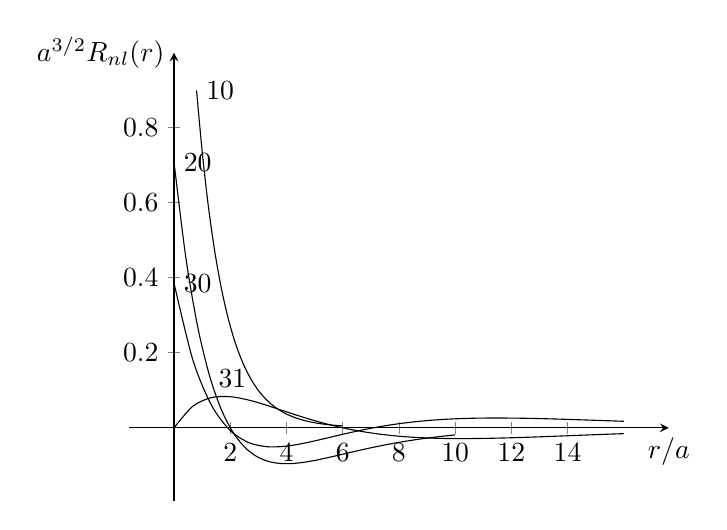
\begin{tikzpicture}[declare function={R10(\x)=2*(e^(-\x));R20(\x)=1/(sqrt(2))*(1-1/2*\x)*e^(-\x/2);R30(\x)=2/sqrt(27)*(1-2/3*\x+2/27*\x^2)*e^(-\x/3);R31(\x)=8/(27*sqrt(6))*(1-\x/6)*\x*e^(-\x/3);}]
\begin{axis}[axis lines=middle,xlabel={$r/a$},ylabel={$a^{3/2}R_{nl}(r)$}, xtick={2,4,6,8,10,12,14},ylabel style={at={(current axis.above origin)},anchor=east},xlabel style={at={(current axis.right of origin)},anchor=north},enlargelimits,ymax=0.9]
\addplot[domain=0.8:6,smooth]{R10(x)}node[pos=0,right]{$10$};
\addplot[domain=0:10,smooth]{R20(x)}node[pos=0,right]{$20$};
\addplot[domain=0:16,smooth]{R30(x)}node[pos=0,right]{$30$};
\addplot[domain=0:16,smooth]{R31(x)}node[pos=0.13,above]{$31$};
\end{axis}
\end{tikzpicture}
\caption{چند ابتدائی ہائیڈروجن رداسی تفاعل موج \عددی{R_{nl}(r)} کی ترسیمات۔}
\label{شکل_تین_ابعادی_چند_رداسی_تفاعل_موج_ہائیڈروجن}
\end{figure}

 \عددی{q} ویں \اصطلاح{لاگیغ کثیر رکنی}\فرہنگ{لاگیغ!کثیر رکنی}\حاشیہب{Laguerre polynomial}\فرہنگ{Laguerre!polynomial} ہے۔\حاشیہد{دیگر علامتوں کی طرح ان کے لئے بھی کئی علامتیں استعمال کی جاتی ہیں۔ میں نے سب سے زیادہ مقبول علامتیں استعمال کی ہیں۔} (جدول \حوالہ{جدول_ابعاد_لاگیغ_ابتدائی_چند} میں چند ابتدائی لاگیغ  کثیر رکنیاں  پیش کی گئی ہیں؛ جدول \حوالہ{جدول_ابعادی_شریک_لاگیغ_کثیر_رکنیاں} میں چند ابتدائی شریک لاگیغ  کثیر رکنیاں پیش کی  گئی ہیں؛  جدول \حوالہ{جدول_ابعادی_ہائیڈروجن_رداسی_تفاعل} میں چند ابتدائی رداسی تفاعلات موج پیش کئے گئے ہیں جنہیں شکل  \حوالہ{شکل_تین_ابعادی_چند_رداسی_تفاعل_موج_ہائیڈروجن}  میں ترسیم کیا گیا ہے۔) ہائیڈروجن کے معمول شدہ تفاعلات موج درجہ ذیل ہیں۔
  \begin{align}\label{مساوات_تین_ابعادی_ہائیڈروجن_تفاعلات_موج}
\psi_{nlm}=\sqrt{\big(\frac{2}{na}\big)^3\frac{(n-l-1)!}{2n[(n+l)!]^{3}}}\,e^{-r/na}\big(\frac{2r}{na}\big)^{l}[L_{n-l-1}^{2l+1}(2r/na)]Y_{l}^{m}(\theta,\phi)
\end{align}
یہ تفاعلات خوفناک نظر آتے ہیں لیکن شکوہ  نہ کیجیے گا؛ یہ اُن چند حقیقی نظاموں میں سے ایک ہے جن کا  بند روپ میں ٹھیک ٹھیک حل حاصل کرنا ممکن ہے۔  دھیان رہے، اگرچہ تفاعلات موج تینوں کوانٹائی اعداد کے تابع ہیں، توانائیوں (مساوات \حوالہ{مساوات_ابعادی_ہائیڈروجن_اجازتی_توانائیاں}) کو صرف \عددی{n} تعین کرتا ہے۔ یہ کولمب توانائی کی ایک مخصوص خاصیت ہے؛ آپ کو یاد ہو گا کہ کروی کنویں  میں توانائیاں \عددی{l} پر منحصر تھیں (مساوات \حوالہ{مساوات_ابعاد_کروی_کنواں_اجازتی_توانائیاں})۔ تفاعلات موج باہمی عمودی 
\begin{align}
\int\psi_{nlm}^{*}\psi_{n'l'm'}r^{2}\sin\theta\dif r\dif\theta\dif\phi=\delta_{nn'}\delta_{ll'}\delta_{mm'} 
\end{align}
ہیں۔ یہ کروی ہارمونیات کی عمودیت (مساوات \حوالہ{مساوات_ابعادی_کروی_ہارمونی_عمودیت})  اور \عددی{(n\neq n')} کی صورت میں  \عددی{H} کی منفرد امتیازی  اقدار کے امتیازی تفاعل ہونے کی بنا پر ہے۔

ہائیڈروجن تفاعلات موج کی تصویر کشی آسان کام نہیں ہے۔  ماہر کیمیا ان کے ایسے کثافتی اشکال بناتے ہیں جن کی چمک  \عددی{\abs{\psi}^{2}}  کا راست متناسب ہوتی ہے (شکل \حوالہء{4.5})۔ زیادہ معلومات مستقل کثافت احتمال کی سطحوں (شکل \حوالہء{4.6}) کے اشکال دیتی ہیں (جنہیں پڑھنا  نسبتاً مشکل ہو گا)۔

%KKK edited with sohail ahmed khan 9 jan 2022

\ابتدا{سوال} 
کلیه توالی( مساوات \حوالہ{مساوات_ابعادی_کلیہ_توالی_کولمب_مخفیہ})  استعمال کرتے ہو ئے  تفاعل موج   \عددی{R_{30}}، \عددی{R_{31}} اور \عددی{R_{32}} حاصل کریں ۔ انہیں معمول پر لانے کی ضرورت نہیں۔ 
\انتہا{سوال}
\ابتدا{سوال}\شناخت{سوال_تین_ابعادی_سائے_دو_صفر_صفر}
\begin{enumerate}[a.]
\item
مساوات  \حوالہ{مساوات_تین_ابعادی_رداسی_بیس}  میں دیے گئے \عددی{R_{20}} کو معمول پر لا کر \عددی{\psi_{200}} تیار کریں ۔
\item
مساوات  \حوالہ{مساوات_تین_ابعادی_رداسی_اکیس}  میں دیے گئے  \عددی{R_{21}}  کو معمول پر لا کر  \عددی{\psi_{211}}،  \عددی{\psi_{210}} اور  \عددی{\psi_{21-1}}  تیار کریں۔ 
\end{enumerate}
\انتہا{سوال}
\ابتدا{سوال} 
\begin{enumerate}[a.]
\item
مساوات  \حوالہ{مساوات_تین_ابعادی_لاگیغ_پ} استعمال کرتے ہوئے ابتدائی چار لاگیغ کثیر رکنیاں حاصل کریں ۔
\item
مساوات  \حوالہ{مساوات_تین_ابعادی_لاگیغ_الف}،  \حوالہ{مساوات_تین_ابعادی_لاگیغ_ب} اور \حوالہ{مساوات_تین_ابعادی_لاگیغ_پ} استعمال کرتے ہوئے  \عددی{n=5} ،    \عددی{l=2} کی صورت میں  \عددی{v(\rho)} تلاش کریں ۔
\item
کلیہ توالی( مساوات \حوالہ{مساوات_ابعادی_کلیہ_توالی_کولمب_مخفیہ})  استعمال کرتے ہوئے \عددی{n=5} ،   \عددی{l=2}  کی صورت میں  \عددی{v(\rho)} تلاش کریں۔ 
\end{enumerate}
\انتہا{سوال}
\ابتدا{سوال} 
\begin{enumerate}[a.]
\item
ہائیڈروجن جو ہر کے زمینی حال میں الیکٹران   کے لیے  \عددی{\langle r \rangle} اور \عددی{\langle r^{2} \rangle} تلاش کریں ۔  اپنے جواب کو رداس بوہر کی صورت میں لکھیں۔ 
\item
ہائیڈروجن جوہر کے زمینی حال میں الیکٹران  کے لیے  \عددی{\langle x \rangle}  اور \عددی{\langle x^{2} \rangle}  تلاش کریں۔  \ترچھا{اشاره :}  آپکو کوئی نیا تکمل حاصل کرنے کی ضرورت نہیں ۔ دھیان  رہے کہ 
  \عددی{r^{2}=x^{2}+y^{2}+z^{2}} ہو گا    ، اور ا  زمینی حال میں تشاکلی کو بروئے کار لائیں۔ 
\item
حال \عددی{n=2} ، \عددی{l=1}، \عددی{m=1} کے لیے \عددی{\langle x^{2} \rangle} تلاش کریں ۔   \ترچھا{انتباہ:}  یہ حال \عددی{x} ، \عددی{y} اور \عددی{z} کے لحاظ سے  تشاکلی نہیں ہے ۔ یہاں
\عددی{x=r\sin{\theta}\cos{\phi}}  استعمال کرنا  ہو گا۔ 
\end{enumerate}
\انتہا{سوال}
\ابتدا{سوال} 
ہائیڈروجن کے زمینی حال میں  \عددی{r} کی کون سی قیمت زیادہ محتمل ہو گی۔ ( اس کا جواب صفر نہیں ہے !)  \ترچھا{اشاره :}  آپکو پہلے  معلوم کرنا ہو گا کہ \عددی{r} اور \عددی{r+\dif{r}} کے بیچ  الیکٹران  پائے جانے کا احتمال کیا ہو گا۔
\انتہا{سوال}
\ابتدا{سوال} 
ہائیڈروجن  جوہر ساکن  حال \عددی{n=2}، \عددی{l=1}، \عددی{m=1}  اور  \عددی{n=2}، \عددی{l=1}، \عددی{m=-1}  کے درج ذیل خطی  مجموعہ   سے ابتداء کرتا ہے ۔
\begin{align*}
\Psi(\kvec{r},0)=\frac{1}{\sqrt{2}}(\psi_{211}+\psi_{21-1})
\end{align*}
\begin{enumerate}[a.]
\item
حال \عددی{\Psi(\kvec{r},t)} تیار کریں ۔ اس کی سادہ ترین صورت حاصل کریں ۔
\item
مخفی توانائی  کی توقعاتی قیمت ی   \عددی{\langle V \rangle} تلاش کریں ۔ (کیا یہ  \عددی{t} کی  تابع ہو گی؟)  اصل کلیہ اور عدد دی جواب   کو الیکٹران وولٹ تو صورت میں پیش کریں ۔
\end{enumerate}
\انتہا{سوال}

\جزوحصہ{ہائیڈروجن  کا   طیف}
اصولی طور پر ایک ہائیڈروجن جوہر جو ساکن حال \عددی{\psi_{nlm}} میں پایا جاتا ہو  ہمیشہ کے لیے اسی حال میں رہے گا۔ تاہم اس کو (  دوسرے جوہر کے ساتھ ٹکرا کر  یا اس پر روشنی  ڈال کر)  چھیڑنے سے الیکٹران کسی دوسرے ساکن حال میں \اصطلاح{عبور}\فرہنگ{عبور}\حاشیہب{transition}\فرہنگ{transition} کر سکتا ہے ۔ یہ توانائی جذب کر کے زیادہ توانائی  حال منتقل ہو سکتا ہے یا   (عموماً   برقناطیسی   نوریہ کے  اخراج   سے)     توانائی خارج کر  کے کم توانائی  حال  منتقل ہو سکتا ہے ۔\حاشیہد{فطراً،   اس میں تابع وقت باہم  عمل پایا جائے گا جس کی تفصیل باب \حوالہ{باب_تابع_وقت_نظریہ_اضطراب} میں پیش کی جائے گی۔یہاں اصل عمل جاننا ضروری نہیں ہے۔} عملاً  ایسی چھیڑخانیاں  ہر وقت پائی جائیں گی لہٰذا عبور (جنہیں  "کوانٹم  چھلانگ" کہتے ہیں)   مستقل طور پر ہوتے  رہیں    گے، جن  کی  بنا پر  ہائیڈروجن  سے ہر وقت   روشنی (نوریہ)  خارج ہو گی جس کی تونائی   ابتدائی اور اختتامی حالات کی  توانائیوں  کے فرق
\begin{align}
E_{\gamma}=E_{i}-E_{f}=\SI{-13.6}{\electronvolt}\,\big(\frac{1}{n^{2}_{i}}-\frac{1}{n^{2}_{f}}\big)
\end{align}
 کے برابر ہو گا ۔
 
اب \اصطلاح{کلیہ پلانک}\فرہنگ{پلانک!کلیہ}\حاشیہب{Planck's formula}\فرہنگ{Planck's!formula}\حاشیہد{نوریہ درحقیقت برقناطیسی اخراج  کا ایک کوانٹم ہے۔یہ ایک اضافیتی  چیز ہے جس پر غیر اضافی کوانٹم میکانیات قابل استعمال نہیں ہے۔اگرچہ ہم چند مواقع پر نوریہ کی بات کرتے ہوئے کلیہ پلانک  سے اس کی توانائی حاصل کریں گے، یاد رہے کہ اس کا اس نظریہ سے کوئی تعلق نہیں جس پر ہم بات کر رہے ہیں۔}  کے تحت  نوریہ  کی توانائی اس کے تعدد کے راست تناسب ہو گی:
\begin{align}
E_{\gamma}=h\nu
\end{align}
جبکہ   \اصطلاح{  طول موج}\فرہنگ{طول موج}    \عددی{\lambda=c/\nu} ہے لہٰذا درج ذیل ہو گا۔
\begin{align}\label{مساوات_تین_ابعادی_رڈبرگ_کلیہ}
\frac{1}{\lambda}=R\big(\frac{1}{n^{2}_{f}}-\frac{1}{n^{2}_{i}}\big)
\end{align}
جہاں 
\begin{align}
R\equiv \frac{m}{4\pi{c}\hslash^{3}}\big(\frac{e^{2}}{4\pi\epsilon_{o}}\big)^{2}=\SI{1.097e7}{\per\meter}
\end{align}
\اصطلاح{رڈبرگ  مستقل}\فرہنگ{رڈبرگ}\حاشیہب{Rydberg constant}\فرہنگ{Rydberg!constant} کہلاتا ہے ۔ مساوات \حوالہ{مساوات_تین_ابعادی_رڈبرگ_کلیہ} ہائیڈروجن کے طیف کا  \اصطلاح{کلیہ رڈبرگ}\فرہنگ{رڈبرگ!کلیہ}\حاشیہب{Rydberg formula}\فرہنگ{Rydberg!formula}  ہے ۔ یہ کلیہ انیسویں  صدی میں تجرباتی طور پر اخذ کیا گیا ۔نظریہ بوہر  کی سب سے بڑی فتح  اس کلیے کا حصول ہے جو قدرت کے بنیادی مستقلات  کی صورت میں \عددی{R}  کی قیمت دیتا ہے۔ زمینی حال  \عددی{(n_{f}=1)}  میں عبور،   بالائے بصری خطہ میں پائے  جاتے  ہیں  جنہیں    طیف پیمائی کار  \اصطلاح{لیمان تسلسل}\فرہنگ{تسلسل!لیمان}\حاشیہب{Lyman series}\فرہنگ{series!Lyman} کہتے ہیں۔ پہلی  ہیجان  حال  \عددی{(n_{f}=2)}
میں عبور،     دکھائی دینے والے خطہ میں  روشنی پیدا  کرتے  ہیں  جسے  \اصطلاح{بالمر تسلسل}\فرہنگ{تسلسل!بالمر}\حاشیہب{Balmer series}\فرہنگ{series!Balmer} کہتے ہیں۔  اسی طرح   \عددی{n_{f}=3}
میں  عبور،  \اصطلاح{پاسشن تسلسل}\فرہنگ{تسلسل!پاسشن}\حاشیہب{Paschen series}\فرہنگ{series!Paschen} دیتے ہیں  جو  زیر  بصری شعاع ہے، وغیرہ وغیرہ  (شکل    \حوالہ{شکل_تین_ابعادی_ہائیڈروجن_طیف}    دیکھیں)۔  (  رہائشی حرارت پر زیادہ تر  ہائیڈروجن  جوہر زمینی حال میں ہونگے؛ اخراجی طیف حاصل کرنے کی خاطر آپکو پہلے مختلف  ہیجان  حالات میں الیکٹران  آباد کرنے ہوں گے؛  ایسا عموماً گیس میں برقی شعلہ   پیدا کر کے کیا جاتا ہے۔)

%fig 4.7

\begin{figure}
\centering
\begin{tikzpicture}[yscale=0.5]
\pgfmathsetmacro{\ea}{-54.4}
\pgfmathsetmacro{\eb}{-13.6}
\pgfmathsetmacro{\ec}{-6.04}
\pgfmathsetmacro{\ed}{-3.4}
\pgfmathsetmacro{\ee}{-1.51}
\pgfmathsetmacro{\ef}{-0.85}
\pgfmathsetmacro{\eg}{-0.54}
%
\draw(0,0)node[left]{$0$}--++(6.5,0)node[above right]{\footnotesize $n$}node[right]{\footnotesize $\infty$};
\draw(0,0)--++(0,-14);
\draw(0.5,\eb)--++(6,0)node[right]{\footnotesize $1$};
\draw(0.5,\ec)--++(6,0)node[right]{\footnotesize $2$};
\draw(0.5,\ed)--++(6,0)node[right]{\footnotesize $3$};
\draw(0.5,\ee)--++(6,0)node[right]{\footnotesize $4$};
\draw(0.5,\ef)--++(6,0)node[right,yshift=-0.1em]{\footnotesize $5$};
\draw(0.5,\eg)--++(6,0)node[right,yshift=0.1em]{\footnotesize $6$};
\foreach \e in {1,2,...,14}{\draw(0,-\e)node[left]{$-\e$}--++(0.1,0);}
\draw[stealth-](1,\eb)--(1,\ec);
\draw[stealth-](1.2,\eb)--(1.2,\ed);
\draw[stealth-](1.4,\eb)--(1.4,\ee);
\draw[stealth-](1.6,\eb)--(1.6,\ef);
\draw[stealth-](1.8,\eb)--(1.8,\eg);
\draw[stealth-](2,\eb)--(2,0);
\draw(1.5,\eb)node[below]{\small{\RL{لیمان تسلسل}}};
\draw[stealth-](3.2,\ec)--(3.2,\ed);
\draw[stealth-](3.4,\ec)--(3.4,\ee);
\draw[stealth-](3.6,\ec)--(3.6,\ef);
\draw[stealth-](3.8,\ec)--(3.8,\eg);
\draw[stealth-](4,\ec)--(4,0);
\draw(3.5,\ec)node[below]{\small{\RL{بالمر تسلسل}}};
\draw[stealth-](5.2,\ed)--(5.2,\ee);
\draw[stealth-](5.4,\ed)--(5.4,\ef);
\draw[stealth-](5.6,\ed)--(5.6,\eg);
\draw[stealth-](5.8,\ed)--(5.8,0);
\draw(5.4,\ed)node[below]{\small{\RL{پاشن تسلسل}}};
\draw(-1,-7)node[rotate=90]{\RL{توانائی \عددی{(\si{\electronvolt})}}};
\end{tikzpicture}
\caption{ہائیڈروجن طیف  میں سطحوط   توانائیاں اور  تحویلات۔}
\label{شکل_تین_ابعادی_ہائیڈروجن_طیف}
\end{figure}

 %===========================
\ابتدا{سوال}\شناخت{سوال_تین_ابعادی_ہائیڈروجنی_جوہر}
\اصطلاح{ہائیڈروجنی جوہر}\فرہنگ{ہائیڈروجنی جوہر}\حاشیہب{hydrogenic atom}\فرہنگ{hydrogenic atom}  \عددی{Z} پروٹان  کے مرکزہ کے گرد طواف کرتے ہوئے  ایک  الیکٹران  پر مشتمل  ہے۔(از  خود ہائیڈروجن  میں  \عددی{Z=1}    جبکہ    باردارہ\اصطلاح{  ہیلیم}\فرہنگ{ہیلیم}\حاشیہب{Helium}\فرہنگ{Helium}  میں  \عددی{Z=2} اور دہری باردارہ   \اصطلاح{لتھیم }\فرہنگ{لتھیم}\حاشیہب{Lithium}\فرہنگ{Lithium} میں  \عددی{Z=3}  ہو گا،  وغیرہ وغیرہ ۔)   ہائیڈروجن  جوہر کی بوہر  توانائیاں  \عددی{E_{n}(Z)}،  بندشی  توانائی\عددی{E_{1}(Z)}،   رداس بوہر  \عددی{a(Z)}،  اور رڈبرگ  مستقل  
\عددی{R(Z)} تعین کریں ۔ (اپنے جوابات کو  ہائیڈروجن  کی متعلقہ قیمتوں کے لحاظ سے پیش کریں۔)   برقناطیسی طیف کے کس خطہ میں  \عددی{Z=2} اور  \عددی{Z=3} کی صورت میں   لیمان   تسلسل پائے جائیں گے؟   \ترچھا{اشارہ :} کسی نئے   حساب کی ضرورت نہیں ہے؛   مخفیہ (  مساوات \حوالہ{مساوات_ابعادی_کولمب_مخفیہ})   میں  \عددی{e^2\to Ze^2}  ہو گا لہٰذا تمام  نتائج میں بھی یہی کچھ پر کرنا  ہو  گا  ۔
\انتہا{سوال}
%==============================
\ابتدا{سوال}
زمین اور سورج کو ہائیڈروجن  جوہر کا متبادل تجاذبی نظام تصور کریں۔
\begin{enumerate}[a.]
\item
 مساوات  \حوالہ{مساوات_ابعادی_کولمب_مخفیہ}  کی جگہ مخفی توانائی تفاعل کیا  ہو گا ؟  (زمین کی کمیت  \عددی{m} جبکہ سورج کی کمیت \عددی{M} لیں۔)
\item
اس نظام کا   "رداس بوہر"  \عددی{a_{g}}  کیا ہو گا؟ اس کی عددی قیمت تلاش کریں ۔
\item
تجاذبی کلیہ  بوہر  لکھ کر  رداس  \عددی{r_0} کے مدار میں سیارہ  کے کلاسیکی توانائی کو  \عددی{E_n} کے برابر رکھ کر  دکھائیں کہ \عددی{n=\sqrt{r_0/a_g}} ہو گا۔ اس سے زمین کے کوانٹائی  عدد  \عددی{n}کی اندازاً قیمت تلاش کریں ۔
\item
فرض کریں  زمین  اگلی نچلی سطح   \عددی{(n-1)} میں عبور کرتی  ہے۔  کتنی توانائی  کا اخراج ہو گا؟  جواب   جاول   میں دیں ۔خارج   نوریہ(یا   زیادہ ممکنہ طور پر \اصطلاح{گریویٹان}\فرہنگ{گریویٹان}\حاشیہب{graviton}\فرہنگ{graviton})   کا طول موج کیا ہو گا؟ ( اپنے جواب کو نوری سالوں میں پیش کریں۔ کیا یہ حیرت انگیز  نتیجہ محض ایک اتفاق ہے ۔)
\end{enumerate}
\انتہا{سوال}

\حصہ{زاویائی معیار حرکت}\شناخت{حصہ_تین_ابعادی_زاویائی_معیار_حرکت}
ہم دیکھ چکے ہیں کہ ہائیڈروجن جو ہر کے ساکن حالات کو تین کوانٹائی اعداد \عددی{n}،  \عددی{l} اور \عددی{m} کے لحاظ سے نام دیا جاتا ہے ۔ صدر کوانٹم عدد  \عددی{(n)} حال کی توانائی تعین کرتا ہے  (مساوات  \حوالہ{مساوات_ابعادی_ہائیڈروجن_اجازتی_توانائیاں})؛  ہم دیکھیں گے کہ \عددی{l} اور \عددی{m} مدارچی زاویائی معیار حرکت سے تعلق رکھتے ہیں ۔ کلاسیکی نظریہ میں وسطی قوتیں،  توانائی اور معیار حرکت بنیادی بقائی مقداریں ہیں ،  اور یہ حیرت کی  بات نہیں  کہ کوانٹم میکانیات میں  زاویائی معیار حرکت( اس سے بھی زیادہ ) اہمیت  رکھتا ہے ۔

 کلاسیکی طور پر  (مبدا کے لحاظ سے)  ایک ذرہ کی زاویائی معیار حرکت درج ذیل کلیہ دیتا ہے 
\begin{align}
\mat{L}=\kvec{r}\times\kvec{p}
\end{align}
جس کے تحت درج ذیل ہو گا۔
\begin{align}\label{مساوات_تین_ابعادی_متعدد_رشتے}
L_{x}=yp_{z}-zp_{y}, \quad\quad L_{y}=zp_{x}-xp_{z}, \quad \quad L_{z}=xp_{y}-yp_{x}
\end{align}
ان کے متعلقہ کوانٹم عاملین معیاری نسخہ \عددی{p_x\to-i\hslash\partial/\partial x}، \عددی{p_y\to-i\hslash\partial/\partial y}،  \عددی{p_z\to-i\hslash\partial/\partial z}  سے حاصل ہوں گے۔ باب   \حوالہ{باب_غیر_تابع_وقت_شروڈنگر_مساوات} میں ہم نے ہارمونی مرتعش کے اجازتی  توانائیوں کو خالص الجبرائی ترکیب سے حاصل کیا۔  اگلے  حصہ میں  الجبرائی ترکیب  استعمال کرتے ہوئے زاویائی معیار حرکت  عاملین کے امتیازی اقدار حاصل کیے جائیں گے۔ یہ ترکیب،  عاملین کے  مقلبیت  تعلقات پر مبنی ہے ۔ اس کے بعد ہم امتیازی تفاعلات حاصل کریں گے جو  زیادہ دشوار کام ہے۔

\جزوحصہ{امتیازی اقدار}
عاملین \عددی{L_{x}} اور \عددی{L_{y}} آپس میں غیر مقلوب  ہیں۔ درحقیقت درج ذیل ہو گا۔\حاشیہد{کوانٹم میکانیات میں تمام عاملین    قانون جزئیتی تقسیم:\عددی{(B+C)=AB+AC} پر پورا اترتے ہیں  (صفحہ \حوالہصفحہ{حاشیہ_تفاعل_موج_عاملین_تبصرہ} پر   حاشیہ \حوالہ{حاشیہ_تفاعل_موج_عاملین_تبصرہ}   دیکھیں)۔ بالخصوص \عددی{[A,B+C]=[A,B]+[A+C]} ہو گا۔}
\begin{gather}
\begin{aligned}
[L_{x},L_{y}]&=[yp_{z}-zp_{y},zp_{x}-xp_{z}]\\
&=[yp_{z},zp_{x}]-[yp_{z},xp_{z}]-[zp_{y},zp_{x}]+[zp_{y},xp_{z}]\\
\end{aligned}
\end{gather}
%===========================
باضابطہ مقلبیت رشتوں  (مساوات \حوالہ{مساوات_تین_ابعادی_باضابطہ_مقلبیت_رشتے})  سے ہم جانتے ہیں کہ صرف \عددی{x} اور \عددی{p_x}،  \عددی{y} اور \عددی{p_y}،  \عددی{z} اور \عددی{p_z} عاملین   غیر مقلوب ہیں۔  یوں درمیانے  دو اجزاء  حذف ہوں گے اور  درج ذیل  رہ جائے گا ۔
\begin{align}
[L_x, L_y] = y p_x [p_z, z] + x p_y [z, p_z] = i \hslash (x p_y - y p_x) = i \hslash L_z
\end{align}
ہم \عددی{[L_y, L_z]} یا \عددی{[L_z, L_x]} بھی تلاش کر سکتے تھے،  تاہم انہیں علیحدہ علیحدہ معلوم کرنے کی ضرورت نہیں ہے؛  ہم اشاریہ کی
 چکری   ادل بدل \عددی{(x \to y, y \to z, z \to x)} سے فوراً درج ذیل لکھ سکتے ہیں 
\begin{align}\label{مساوات_تین_ابعادی_بنیادی_مقلبیت_رشتہ}
[L_x, L_y] = i \hslash L_z ; \quad [L_y, L_z] = i \hslash L_x ; \quad [L_z, L_x] = i \hslash L_y
\end{align}
جو زاویائی معیار حرکت کیے   \اصطلاح{بنیادی مقلبیت رشتے }\فرہنگ{مقلبیت!بنیادی رشتے}\حاشیہب{fundamental commutation relations}\فرہنگ{commutation!fundamental relations}ہیں جن سے باقی سب کچھ اخذ ہوتا ہے۔

 دھیان رہے کہ \عددی{L_x} \عددی{L_y} اور \عددی{L_z} غیر  ہم آہنگ قابل مشاہدہ ہیں۔ متعمم اصول عدم یقینیت (مساوات\حوالہ{مساوات_قواعد_عمومی_اصول_عدم_یقینیت_الف_بے}) کے تحت 
\begin{align*}
\sigma_{L_x}^2 \sigma_{L_y}^2 \ge \big ( \frac{1}{2i} \langle i \hslash L_z \rangle \big )^2 = \frac{\hslash^2}{4} \langle L_z \rangle^2
\end{align*}
یا 
\begin{align}\label{مساوات_تین_ابعادی_عدم_یقینیت}
\sigma_{L_x} \sigma_{L_y} \ge \frac{\hslash}{2} \abs{\langle L_z \rangle}
\end{align}
ہوگا۔  یوں ایسے حالات کی تلاش جو \عددی{L_x} اور \عددی{L_y} کے بیک وقت امتیازی تفاعلات ہوں بے مقصد ہوگا۔ اس کے برعکس کل زاویائی معیار حرکت کا مربع: 
\begin{align}
L^2 \equiv L_x^2 + L_y^2 + L_z^2
\end{align} 
عامل \عددی{L_x} کے ساتھ مقلوب ہے ۔
\begin{align*}
[L^2, L_x] &= [L_x^2, L_x] + [L_y^2, L_x] + [L_z^2, L_x] \\
&= L_y [L_y, L_x] + [L_y, L_x] L_y + L_z [L_z, L_x] + [L_z, L_x] L_z \\
&= L_y (- i \hslash L_z) + (- i \hslash L_z) L_y + L_z (i \hslash L_y) + (i \hslash L_y) L_z \\
&= 0
\end{align*}
(مقالب  کی سادہ روپ حاصل کرنے کے لیے میں نے مساوات\حوالہ{مساوات_قواعد_ایک_مقالب_مماثل} استعمال کیا؛  یہ بھی یاد رہے کہ ہر عامل اپنے  آپ کے  ساتھ مقلوب ہوگا۔)  اس سے آپ اخذ کر سکتے ہیں کہ \عددی{L_y} اور \عددی{L_z} کے ساتھ بھی \عددی{L^2} مقلوب ہوگا 
\begin{align}
[L^2, L_x] = 0, \quad [L^2, L_y] = 0, \quad [L^2, L_z] = 0
\end{align}
یا مختصراً درج ذیل ہوگا ۔
\begin{align}\label{مساوات_تین_ابعادی_مربع_قالب_صفر_مقلوب}
[L^2, \mat{L}] = 0
\end{align} 
اس طرح \عددی{\mat{L}} کے ہر جزو کے ساتھ \عددی{L^2} ہم آہنگ ہوگا اور ہم \عددی{L^2} کا  (مثلاً )  \عددی{L_z} کے ساتھ بیک وقت امتیازی حالات
\begin{align}
L^2 f = \lambda f \quad & \text{\RL{ اور}} \quad L_z f = \mu f 
\end{align}
 تلاش کرنے کی امید رکھ سکتے ہیں۔ ہم نے حصہ  \حوالہ{حصہ_غیر_تابع_وقت_شروڈنگر_الجبرائی_ترکیب}  میں ہارمونی مرتعش پر سیڑھی عامل کی ترکیب استعمال کی۔  اس طرح کی  ترکیب یہاں  بھی استعمال کرتے ہیں ۔یہاں ہم درج ذیل لیتے ہیں ۔
\begin{align}
L \pm \equiv L_x \pm i L_y
\end{align}
\عددی{L_z} کے ساتھ  مقلب درج ذیل ہوگا 
\begin{align*} 
[L_z, L_{\pm}] = [L_z, L_x] \pm i [L_z, L_y] = i \hslash L_y \pm i (- i \hslash L_x) = \pm \hslash (L_x \pm i L_y)
\end{align*}
لہٰذا 
\begin{align}\label{مساوات_تین_ابعادی_ایک_اور_سیڑھی}
[L_z, L_{\pm}] = \pm \hslash L_{\pm}
\end{align}
اور، ظاہر ہے کہ،  درج ذیل ہو گا۔ 
\begin{align}\label{مساوات_تین_ابعادی_مربع_اور_سیڑھی}
[L^2, L_{\pm}] = 0
\end{align}
میں  دعویٰ کرتا ہوں کہ اگر \عددی{L^2} اور \عددی{L_z} کا امتیازی تفاعل \عددی{f} ہو تب \عددی{L_{\pm} (f)} بھی ان کا امتیازی تفاعل ہوگا:  مساوات\حوالہ{مساوات_تین_ابعادی_مربع_اور_سیڑھی}  درج ذیل کہتی ہے 
\begin{align}
L^2 (L_{\pm} f) = L_{\pm} (L^2 f) = L_{\pm} (\lambda f) = \lambda (L_{\pm} f)
\end{align}
لہٰذا اسی امتیازی قدر \عددی{\lambda} کے لیے \عددی{L_{\pm} f} بھی \عددی{L^2} کا امتیازی تفاعل ہوگا، اور  مساوات \حوالہ{مساوات_تین_ابعادی_ایک_اور_سیڑھی} درج ذیل کہتی ہے  
\begin{align}
L_z (L_{\pm} f) &= (L_z L_{\pm} - L_{\pm} L_z) f + L_{\pm} L_z f = \pm \hslash L_\pm f + L_{\pm} (\mu f) \nonumber \\
&= (\mu \pm \hslash ) (L_{\pm} f)
\end{align}
لہٰذا نئے  امتیازی قدر \عددی{\mu \pm \hslash} کے لیے   \عددی{L_z} کا  \عددی{L_{\pm} f} امتیازی تفاعل ہوگا۔  ہم \عددی{L_{+}} کو \اصطلاح{عامل رفعت}\فرہنگ{عامل!رفعت}\حاشیہب{raising operator}\فرہنگ{operator!raising} کہتے ہیں چونکہ یہ \عددی{L_{z}} کے امتیازی قدر کو \عددی{\hslash}  بڑھاتا ہے جبکہ \عددی{L_{-}} \اصطلاح{عامل تقلیل}\فرہنگ{عامل!تقلیل}\حاشیہب{lowering operator}\فرہنگ{operator!lowering} کہلاتا ہے چونکہ یہ امتیازی قیمت کو \عددی{\hslash} کم کرتا ہے۔

 یوں ہمیں \عددی{\lambda} کی کسی ایک قیمت کے لیے، حالات کی ایک سیڑھی ملتی ہے،  جس کا ہر پایہ قریبی پایہ سے \عددی{L_{z}} کی امتیازی قدر کے لحاظ سے \عددی{\hslash} کی ایک اکائی  فاصلہ پر ہوگا  (شکل  \حوالہ{تین_ابعادی_زاویائی_معیار_اثر_سیڑھی})۔   سیڑھی چڑھنے کی خاطر ہم عامل رفت کا اطلاق کرتے ہیں جبکہ سیڑھی اترنے کی خاطر ہم عامل تقلیل لاگو کرتے ہیں۔ تاہم یہ عمل ہمیشہ کے لئے برقرار نہیں رہ سکتا ہے۔ ہم آخرکار  ایک ایسے حال تک پہنچے گے جس کا \عددی{z} جزو \ترچھا{کل} سے زیادہ ہوگا جو ایک ناممکن صورت\حاشیہد{باضابطہ طور پر 
 \عددی{\langle L^2\rangle=\langle L_x^2\rangle+\langle L_y^2\rangle+\langle L_z^2\rangle}
ہو گا، لیکن 
\عددی{\langle L_x^2\rangle=\langle f|L_x^2 f\rangle=\langle L_x f| L_x f\rangle\ge 0}
 ہے  (اور \عددی{L_y} کے لئے بھی ایسا ہی ہو گا ) لہٰذا 
\عددی{\lambda=\langle L_x^2 \rangle+\langle L_y^2\rangle+\mu^2 \ge \mu^2}
  ہو گا۔ } ہے ۔لازماً سیڑھی کا ایسا  " بالا    ترین پایہ"  \عددی{f_{t}}،  پایا جائے گا جو  درج ذیل کو مطمئن\حاشیہد{درحقیقت، ہم صرف اتنا اخذ کر سکتے ہیں کہ \عددی{L_+f_t} معمول پر لانے کے قابل نہیں ہے؛اس کا   معیار صفر کی بجائے لامتناہی ہو سکتا ہے۔ سوال \حوالہ{سوال_تین_ابعادی_معیار_لامتناہی_ہو_سکتا_ہے} میں  اس پر غور کیا گیا ہے۔} کرے گا۔
\begin{align}
L_{+} f_{t} = 0
\end{align}
%
\begin{figure}
\centering
\begin{tikzpicture}
\pgfmathsetmacro{\a}{70}
\pgfmathsetmacro{\s}{0.5}
\draw(0,0)--++(\a:12*\s)--++(-0.1,0)--++(\a:-12*\s)--++(0.1,0);
\draw(1,0)--++(\a:12*\s)--++(0.1,0)--++(\a:-12*\s)--++(-0.1,0);
\foreach \n in {1,2,...,11}{\draw(\a:\n*\s)--++(1,0);\draw(\a:\n*\s+0.1*\s)--++(1,0);}
\draw(\a:\s)++(-0.1,0)node[left]{$\bar{l}\hslash$} ++(1.2,0)node[right]{$f_b$};
\draw(\a:3*\s)++(-0.1,0)node[left]{$\mu-3\hslash$} ++(1.2,0)node[right]{$L_{-}^3 f$};
\draw(\a:4*\s)++(-0.1,0)node[left]{$\mu-2\hslash$} ++(1.2,0)node[right]{$L_{-}^2 f$};
\draw(\a:5*\s)++(-0.1,0)node[left]{$\mu-\hslash$} ++(1.2,0)node[right]{$L_{-} f$};
\draw(\a:6*\s)++(-0.1,0)node[left]{$\mu$} ++(1.2,0)node[right]{$f$};
\draw(\a:7*\s)++(-0.1,0)node[left]{$\mu+\hslash$} ++(1.2,0)node[right]{$L_{+} f$};
\draw(\a:8*\s)++(-0.1,0)node[left]{$\mu+2\hslash$} ++(1.2,0)node[right]{$L_{+}^2 f$};
\draw(\a:9*\s)++(-0.1,0)node[left]{$\mu+3\hslash$} ++(1.2,0)node[right]{$L_{+}^3 f$};
\draw(\a:11*\s)++(-0.1,0)node[left]{$l \hslash$} ++(1.2,0)node[right]{$f_t$};
\draw[ultra thick,stealth-]($(\a:1.5*\s)+(2.5,0)$)node[right]{$L_{-}$}--++(\a:\s);
\draw[ultra thick,-stealth]($(\a:9.25*\s)+(2.5,0)$)--++(\a:\s)node[right]{$L_{+}$};
\end{tikzpicture}
\caption{زاویائی معیار حرکت  حالات  کی "سیڑھی"۔}
\label{تین_ابعادی_زاویائی_معیار_اثر_سیڑھی}
\end{figure}
فرض کریں اس بالا ترین  پایہ پر \عددی{L_z} کی امتیازی قیمت \عددی{\hslash l} ہو (حرف \عددی{"l"} کی مناسبت آپ پر جلد آیا ہوں گی)۔ 
\begin{align}
L_z f_t = \hslash l f_{t}; \quad L^2 f_t = \lambda f_t
\end{align}
اب درج ذیل ہوگا 
\begin{align*} 
L_{\pm} L_{\mp}&= (L_x \pm i L_y) (L_x \mp i L_y) = L_x^2 + L_y^2 \mp i (L_x L_y - L_y L_x) \\
&= L^2 - L_z^2 \mp i (i \hslash L_z)
\end{align*}
یا دوسرے الفاظ میں درج ذیل ہوگا ۔
\begin{align}\label{مساوات_تین_ابعادی_مربع_بصورت_رفعت}
L^2 = L_{\pm} L_{\mp} + L_z^2 \mp \hslash L_z
\end{align}
یوں 
\begin{align*}
L^2 f_t = (L_{-} L_{+} + L_z^2 + \hslash L_z) f_t = (0 + \hslash^2 l^2 + \hslash^2 l) f_t = \hslash^2 l (l + 1) f_t
\end{align*}
لہٰذا درج ذیل ہوگا ۔
\begin{align}\label{مساوات_تین_ابعادی_لمڈا_تعلق_الف}
\lambda = \hslash^2 l (l + 1)
\end{align}
یہ ہمیں \عددی{L_z} کی امتیازی قدر کی زیادہ سے زیادہ قیمت کی صورت میں \عددی{L^2} کی امتیازی قدر دیتی ہے۔

 ساتھ ہی،  اسی وجہ کی بنا،  سیڑھی کا  نچلا ترین  پایہ \عددی{f_b} بھی پایا جائے گا جو درج ذیل کو مطمئن کرے گا۔ 
\begin{align}
L_{-} f_b = 0
\end{align}
فرض کریں اس نچلے ترین  پایہ پر \عددی{L_z} کا امتیازی قدر \عددی{
\hslash \bar{l}
} ہو :
\begin{align}
L_z f_b = \hslash \bar{l} f_b ; \quad L^2 f_b = \lambda f_b
\end{align}
مساوات \حوالہ{مساوات_تین_ابعادی_مربع_بصورت_رفعت} استعمال کرتے ہوئے
\begin{align*}
L^2 f_b = (L_{+} L_{-} + L_z^2 - \hslash L_z ) f_b = (0 + \hslash^2 \bar{l}^{2} - \hslash^2 \bar{l}) f_b = \hslash^2 \bar{l} (\bar{l} - 1) f_b
\end{align*}
لہٰذا درج ذیل ہوگا ۔
\begin{align}\label{مساوات_تین_ابعادی_لمڈا_تعلق_ب}
\lambda = \hslash^2 \bar{l} (\bar{l} - 1)
\end{align}
مساوات  \حوالہ{مساوات_تین_ابعادی_لمڈا_تعلق_الف}  اور مساوات \حوالہ{مساوات_تین_ابعادی_لمڈا_تعلق_ب} کا موازنہ کرنے سے \عددی{
l (l + 1) = \bar{l} (\bar{l} - 1)
} ہوگا لہٰذا یا \عددی{
\bar{l} = l + 1
} ہوگا   (جو بے معنی ہے ، چونکہ نچلا ترین  پایہ، بالا ترین   پایہ سے  بلند نہیں ہو سکتا)  یا درج ذیل ہوگا ۔
\begin{align}
\bar{l} = - l
\end{align}

ظاہر ہے کہ \عددی{L_z} کے امتیازی اقدار \عددی{m \hslash} ہونگے،  جہاں \عددی{ m} (اس حرف  کی مناسبت آپ پر جلد عیاں ہو گی) کی قیمت \عددی{ N} عدد صحیح  قدم لیتے ہوئے  \عددی{- l} تا \عددی{+ l} ہوگی۔ بالخصوص آپ دیکھ سکتے ہیں کہ \عددی{
l = - l + N
} یعنی  \عددی{
l = N/2
} ہوگا،   لہٰذا   \عددی{l} لازماً \ترچھا{ عدد صحیح} یا \ترچھا{ نصف عدد صحیح}  ہوگا۔ امتیازی تفاعلات کی تصویر کشی  اعداد \عددی{l} اور \عددی{ m}  کرتے ہیں: 
\begin{align}
L^2 f_l^m = \hslash^2 l (l + 1) f_l^m ; \quad L_z f_l^m = \hslash m f_l^m
\end{align}
جہاں درج ذیل ہونگے ۔
\begin{align}\label{مساوات_تین_ابعادی_نصف_عدد_صحیح_قیمتیں}
l = 0, \frac{1}{2}, 1,\frac{3}{2}, \dotsc ; \quad m = - l, - l + 1, \dotsc , l - 1, l
\end{align}
\عددی{l} کی کسی ایک قیمت کے لیے \عددی{m} کی \عددی{2l + 1} مختلف قیمتیں ہوں گی ( یعنی سیڑھی کے \عددی{2l + 1} پائے  ہونگے)۔
\begin{figure}
\centering
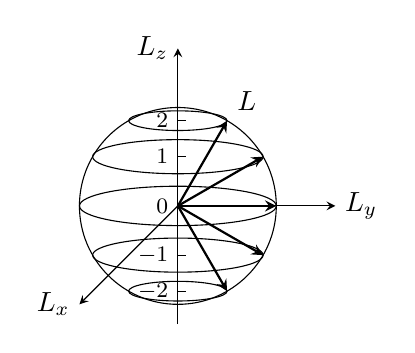
\begin{tikzpicture}
\pgfmathsetmacro{\a}{30}
\pgfmathsetmacro{\r}{1.25}
\pgfmathsetmacro{\ra}{\r*sin(\a)}
\pgfmathsetmacro{\ha}{\r*cos(\a)}
\pgfmathsetmacro{\rb}{\r*sin(2*\a)}
\pgfmathsetmacro{\hb}{\r*cos(2*\a)}
\pgfmathsetmacro{\rc}{\r*sin(3*\a)}
\pgfmathsetmacro{\hc}{\r*cos(3*\a)}
\draw[-stealth](0,0)--++(-1.25,-1.25)node[left]{$L_x$};
\draw[-stealth](0,0)--++(2,0)node[right]{$L_y$};
\draw[-stealth](0,-1.5)--(0,2)node[left]{$L_z$};
\draw(0,0) circle (\r);
\draw(0,\ha) circle (\ra cm and 0.20*\ra cm);
\draw(0,\hb) circle (\rb cm and 0.20*\rb cm);
\draw(0,\hc) circle (\rc cm and 0.20*\rc cm);
\draw(0,-\ha) circle (\ra cm and 0.20*\ra cm);
\draw(0,-\hb) circle (\rb cm and 0.20*\rb cm);
\draw(0,\ha)node[left]{\footnotesize$2$}--++(0.1,0);
\draw(0,\hb)node[left]{\footnotesize$1$}--++(0.1,0);
\draw(0,0)node[left]{\footnotesize$0$};
\draw(0,-\ha)node[left]{\footnotesize$-2$}--++(0.1,0);
\draw(0,-\hb)node[left]{\footnotesize$-1$}--++(0.1,0);
\draw[-stealth,thick](0,0)--++(2*\a:\r)node[above right]{$\mat{L}$};
\draw[-stealth,thick](0,0)--++(\a:\r);
\draw[-stealth,thick](0,0)--++(0:\r);
\draw[-stealth,thick](0,0)--++(-\a:\r);
\draw[-stealth,thick](0,0)--++(-2*\a:\r);
\end{tikzpicture}
\caption{زاویائی معیار حرکت  حالات (برائے \عددی{l=2})۔}
\label{تین_ابعادی_زاویائی_معیار_حرکت_حالات}
\end{figure}

 بعض اوقات اس نتیجہ کو شکل \حوالہ{تین_ابعادی_زاویائی_معیار_حرکت_حالات} کی طرز پر ظاہر کیا جاتا ہے ( جو \عددی{l = 2} کے لیے دکھایا گیا ہے)۔ یہاں تیر کے نشان ممکنہ زاویائی  معیار حرکت کو ظاہر کرتے ہیں؛  ان تمام کی لمبائیاں  \عددی{\hslash} کی اکائیوں میں \عددی{\sqrt{l (l+ 1)}} ہوگی جو (یہاں \عددی{
\sqrt{6} = 2.45
} ہے)  جبکہ  ان  کے \عددی{z} اجزاء \عددی{m} کی اجازتی قیمتیں (\عددی{-2}، \عددی{-1}، \عددی{0}، \عددی{1}، \عددی{2})  ہیں۔  دھیان رہے کہ ان سمتیات  کے مقدار (  یعنی کرہ کا رداس)،   \عددی{z} جزو کی زیادہ سے زیادہ قیمت سے بڑا ہے! (  ماسوائے \عددی{l = 0} کی" حقیر"  صورت میں،   عموماً \عددی{\sqrt{l (l + 1)} > l} ہوگا۔  )  آپ دیکھ سکتے ہیں کہ آپ زاویائی معیار حرکت کو سیدھا  \عددی{z} رخ نہیں رکھ سکتے ہیں۔ پہلی نظر میں یہ ایک نا معقول بات نظر آتی ہے۔ "کیا میں \عددی{z} محدد کو زاویائی معیار حرکت سمتیہ کے رخ منتخب نہیں کر سکتا ہوں ؟"اب ایسا کرنے کی خاطر آپ کو تینوں اجزاء بیک وقت معلوم ہونے چاہیے ہیں جبکہ اصول عدم یقینیت  (مساوات  \حوالہ{مساوات_تین_ابعادی_عدم_یقینیت})   کہتی ہے کہ یہ ناممکن ہے۔  چلو  مان لیا لیکن کیا یہ بھی ممکن نہیں ہے کہ میں اتفاقاً  \عددی{z} محدد کو \عددی{\mat{L}} کے رخ منتخب  کر    لوں؟     بالکل نہیں!  آپ بنیادی نکتہ نہیں سمجھ پائے  ہیں۔  ایسا نہیں ہے کے  محض آپ  \عددی{\mat{L}} کے تینوں اجزاء نہیں جانتے ہیں بلکہ ایک ذرے   کا   تعیین زاویائی معیار حرکت سمتیہ  ہو ہی  نہیں  سکتا ہے؛  جیسا کہ اس کا مقام اور معیار حرکت بیک وقت تعیین  نہیں ہو سکتے ہیں۔ اگر \عددی{L_z} کی قیمت  ہمیں ٹھیک ٹھیک معلوم ہو تب \عددی{L_x} اور \عددی{L_y} ہم  نہیں جان سکتے ہیں  شکل  \حوالہ{تین_ابعادی_زاویائی_معیار_حرکت_حالات}  میں سمتیات گمراہ کن ہیں؛  بہتر ہوتا کہ خطوط عرض بلند پر  ان کی لپائی کی جاتی جو یہ ظاہر کرتی کہ \عددی{L_x} اور \عددی{L_y} غیر تعیین  ہیں۔

 میں امید کرتا ہوں کہ میں آپ کو متاثر کرنے میں کامیاب ہوا ہوں گا۔  زاویائی معیار حرکت کے بنیادی مقلبیت رشتوں   (مساوات \حوالہ{مساوات_تین_ابعادی_بنیادی_مقلبیت_رشتہ}) سے آغاز کرتے ہوئے ہم نے،  صرف الجبرائی تراکیب استعمال کرکے،  امتیازی تفاعلات دیکھے بغیر،  \عددی{L^2} اور \عددی{L_z} کے امتیازی اقدار تعین کیے۔ آئیں  اب امتیازی تفاعلات تیار کریں؛  جو  آپ دیکھیں گے اتنا آسان نہیں ہوگا۔ میں  کانٹے  کی بات    \عددی{
f_l^m = Y_l^m
} سے شروع کرتا ہوں؛  \عددی{L^2} اور \عددی{L_z} کے  امتیازی تفاعلات وہی کروی ہارمونیات ہیں جنہیں ایک دوسری راہ پر چلتے ہوئے ہم نے حصہ \حوالہ{حصہ_تین_ابعادی_زاویائی_مساوات} میں حاصل کیا (  یہی وجہ ہے کہ میں نے حرف \عددی{l} اور \عددی{m} استعمال کیے)۔  اب میں آپ کو بتا  سکتا ہوں  کہ کروی ہارمونیات کیوں عمودی ہیں۔ یہ الگ تھلگ امتیازی اقدار کے ہرمشی عاملین ( \عددی{L^2} اور \عددی{L_z})  کے امتیازی تفاعلات ہیں (حصہ \حوالہ{حصہ_قواعد_غیر_مسلسل_طیف} میں مسئلہ \حوالہ{مسئلہ_قواعد_انفرادی_اقدار_عمودی_تفاعلات})۔ 

\ابتدا{سوال}\شناخت{سوال_تین_ابعادی_معیار_لامتناہی_ہو_سکتا_ہے}
عامل رفت اور عامل تقلیل \عددی{ m} کی قیمت ایک \عددی{(1)} سے تبدیل کرتے ہیں 
\begin{align}\label{مساوات_تین_ابعاد_عامل_تقلیل_رفعت_اکائی_تبدیلی}
L_{\pm} f_l^m = (A_l^m) f_l^{m \pm 1}
\end{align}
جہاں \عددی{A_l^m} کوئی مستقل ہے۔ \ترچھا{سوال:} امتیازی تفاعلات کو معمول پر لانے کی خاطر \عددی{A_l^m} کیا ہوگا؟ \ترچھا{ اشارہ:}  پہلے دکھائیں کہ \عددی{L_{\pm}} اور \عددی{L_{\mp}} ایک دوسرے کے ہرمشی جوڑی دار ہیں ( چونکہ \عددی{L_x} اور \عددی{L_y} قابل مشاہدہ  ہیں،  آپ فرض کر سکتے ہیں یہ ہرمشی ہوں گے لیکن آپ چاہیں تو اس کی ثابت کر سکتے ہیں) ؛ اور   اس کے بعد مساوات  \حوالہ{مساوات_تین_ابعادی_مربع_بصورت_رفعت}  استعمال کریں۔ \ترچھا{ جواب:} 
\begin{align}\label{مساوات_تین_ابعادی_اے_ایل_ایم}
A_l^m = \hslash \sqrt{l (l +1) - m (m \pm 1)} = \hslash \sqrt{(l \mp m)(l \pm m + 1)} 
\end{align}
دیکھیے گا کے سیڑھی کی بلند ترین اور نچلے ترین پایہ پر کیا ہوگا ( جب آپ \عددی{f_l^l} پر \عددی{L_{+}} یا \عددی{f_l^{-l}} پر \عددی{L_{-}} لاگو کرتے ہیں)۔ 
\انتہا{سوال}
\ابتدا{سوال}
\begin{enumerate}[a.]
\item
مقام اور معیار حرکت کی باضابطہ  مقلبیت رشتوں   مساوات  \حوالہ{مساوات_تین_ابعادی_باضابطہ_مقلبیت_رشتے}  سے آغاز  کرتے ہوئے درج ذیل مقالب  حاصل کریں ۔
\begin{gather}
\begin{aligned}
[L_z , x] = i \hslash y, & \quad [L_z , y] = - i \hslash x, \quad  [L_z , z] = 0, \\
 [L_z , p_x] = i \hslash p_y ,   &\quad [L_z , p_y] = - i \hslash p_x , \quad [L_z , p_z] = 0
\end{aligned}
\end{gather}
\item
ان نتائج کو استعمال کرتے ہوئے مساوات  \حوالہ{مساوات_تین_ابعادی_متعدد_رشتے}  سے  \عددی{[L_z , L_x] = i \hslash L_y} حاصل کریں ۔
\item
مقالب  \عددی{[L_z , r^2]} اور \عددی{[L_z , p^2]} کی قیمتیں( جہاں \عددی{r^2 = x^2 + y^2 + z^2} اور \عددی{p^2 = p_x^2 + p_y^2 + p_z^2} ہیں)  تلاش کریں۔
\item
اگر \عددی{V} صرف \عددی{r} کا تابع ہو تب دکھائیں کے ہیملٹنی \عددی{H = (p^2 /2m) + V} زاویائی عامل  \عددی{\mat{L}} کے  تینوں اجزاء کے ساتھ مقلوبی  ہوگا۔ یوں \عددی{ H}،  \عددی{L^2} اور \عددی{L_z} باہمی ہم آہنگ  قابل مشاہدہ  ہوں گے ۔
\end{enumerate}
\انتہا{سوال}
\ابتدا{سوال}\شناخت{سوال_تین_ابعادی_مسئلہ_اہرنفسٹ}
\begin{enumerate}[a.]
\item
دکھائیں کہ  مخفیہ   \عددی{V(\kvec{r})} میں ایک ذرے کی مدارچی زاویائی معیار حرکت \عددی{\mat{L}} کی توقعاتی قیمت کی شرح  تبدیلی اس کے قوت مروڑ کی توقعاتی قیمت کے برابر ہوگی 
\begin{align*}
\frac{\dif}{\dif t} \langle \mat{L} \rangle = \langle \mat{N} \rangle
\end{align*}
جہاں  درج ذیل ہے۔
\begin{align*}
\mat{N} = \kvec{r} \times (- \nabla V)
\end{align*}
(یہ مسئلہ اہرنفسٹ کا مماثل گھومتا تعلق ہے ۔)
\item
دکھائیں کہ  کسی بھی کروی تشاکلی مخفیہ کے لیے \عددی{
\dif \langle \mat{L} \rangle \dif t = 0
} ہوگا۔ (یہ \اصطلاح{زاویائی معیار حرکت کی بقا}\فرہنگ{زاویائی معیار حرکت! بقا}\حاشیہب{conservation of angular momentum}\فرہنگ{angular momentum!conservation} کا کوانٹم میکانی روپ ہے۔) 
\end{enumerate}
\انتہا{سوال}

%the above is prob 4.20 (p179)
%===============

\جزوحصہ{امتیازی تفاعلات}
ہمیں سب سے پہلے \عددی{L_x}،  \عددی{L_y} اور \عددی{L_z} کو کروی محدد میں لکھنا ہوگا اب  \عددی{\mat{L} = (\hslash/i)(\kvec{r} \times \kvec{\nabla})} ہے جبکہ کروی محدد میں ڈھلوان درج ذیل ہوگا 
\begin{align}
\kvec{\nabla} = \ar \frac{\partial}{\partial r} + \atheta \frac{1}{r} \frac{\partial}{\partial \theta} + \aphi \frac{1}{r \sin {\theta}} \frac{\partial}{\partial \phi}
\end{align}
جہاں \عددی{\kvec{r} = r \ar} ہے۔ یوں درج ذیل لکھا جا سکتا ہے ۔
\begin{align*}
\mat{L} = \frac{\hslash}{i} \big [ r (\ar \times \ar) \frac{\partial}{\partial r} + (\ar \times \atheta) \frac{\partial}{\partial \theta} + (\ar \times \aphi) \frac{1}{\sin \theta} \frac{\partial}{\partial \phi} \big ]
\end{align*}
اب \عددی{(\ar \times \ar) = 0}،  \عددی{(\ar \times \atheta) = \aphi} اور \عددی{(\ar \times \aphi) = - \atheta} ہوتے
 ہیں( شکل \حوالہ{شکل_تین_ابعادی_کروی_محدد_تعریف})   لہٰذا درج ذیل ہوگا۔ 
\begin{align}
\mat{L} = \frac{\hslash}{i} \big ( \aphi \frac{\partial}{\partial \theta} - \atheta \frac{1}{\sin \theta} \frac{\partial}{\partial \phi} \big )
\end{align}
اکائی  سمتیات \عددی{\atheta} اور \عددی{\aphi} کو ان کے کارتیسی اجزاء میں لکھتے ہیں۔ 
\begin{align}
\atheta = (\cos \theta \cos \phi) \ai + (\cos \theta \sin \phi) \aj - (\sin \theta) \ak
\end{align}
\begin{align}
\aphi = - (\sin \phi) \ai + (\cos \phi) \aj
\end{align}
یوں 
\begin{align*}
\mat{L} = \frac{\hslash}{i} [(- \sin \phi \,\ai + \cos \phi\, \aj) \frac{\partial}{\partial \theta} - (\cos \theta \cos \phi \,\ai + \cos \theta \sin \phi \,\aj - \sin \theta \,\ak) \frac{1}{\sin \theta} \frac{\partial}{\phi}]
\end{align*}
ہوگا ظاہر ہے درج ذیل ہوں گے ۔
\begin{align}
L_x &= \frac{\hslash}{i} \big ( - \sin \phi \frac{\partial}{\partial \theta} - \cos \phi \cot \theta \frac{\partial}{\partial \phi} \big )\\
L_y &= \frac{\hslash}{i} \big ( + \cos \phi \frac{\partial}{\partial \theta} - \sin \phi \cot \theta \frac{\partial}{\partial \phi} \big )\\
L_z &= \frac{\hslash}{i} \frac{\partial}{\partial \phi}\label{مساوات_تین_ابعادی_زیڈ_عامل}
\end{align} 

ہمیں عامل رفت اور عامل تقلیل بھی درکار ہوں گے: 
\begin{align*}
L_{\pm} = L_x \pm i L_y = \frac{\hslash}{i} \big [ (- \sin \phi \pm i \cos \phi) \frac{\partial}{\partial \theta} - (\cos \phi \pm i \sin \phi) \cot \theta \frac{\partial}{\partial \phi} \big ]
\end{align*}
تاہم  \عددی{\cos \phi \pm i \sin \phi = e^{\pm i \phi}} ہوتا ہے لہٰذا درج ذیل ہوگا ۔
\begin{align}\label{مساوات_تین_ابعادی_سیڑھی_عاملین}
L_{\pm} = \pm \hslash e^{\pm i \phi} \big ( \frac{\partial}{\partial \theta} \pm i \cot \theta \frac{\partial}{\partial \phi} \big )
\end{align}
بالخصوص (سوال \حوالہ{سوال_تین_ابعادی_معمول_زنی}-ا ) درج ذیل 
\begin{align}\label{مساوات_تین_ابعادی_سیڑھی_عاملین_آگے_پیچے}
L_{+} L_{-} = - \hslash^2 \big ( \frac{\partial^2}{\partial \theta^2} + \cot \theta \frac{\partial}{\partial \theta} + \cot^2 \theta \frac{\partial^2}{\partial \phi^2} + i \frac{\partial}{\partial \phi} \big )
\end{align}
لہٰذا  (سوال \حوالہ{سوال_تین_ابعادی_معمول_زنی}-ب)درج ذیل حاصل ہو گا ۔
\begin{align}\label{مساوات_تین_ابعادی_مربع_معیار_حرکت}
L^2 = - \hslash^2 \big [ \frac{1}{\sin \theta} \frac{\partial}{\partial \theta} \big ( \sin \theta \frac{\partial}{\partial \theta} \big ) + \frac{1}{\sin^2 \theta} \frac{\partial^2}{\partial \phi^2} \big ]
\end{align}

ہم اب \عددی{f_l^m (\theta, \phi)  } تعین کر سکتے ہیں۔  یہ \عددی{L^2} کا امتیازی تفاعل ہے،  جس کا  امتیازی قدر \عددی{\hslash^2 l (l + 1)} ہے۔
\begin{align*}
L^2 f_l^m = - \hslash^2 \big [ \frac{1}{\sin \theta} \frac{\partial}{\partial \theta} \big ( \sin \theta \frac{\partial}{\partial \theta} \big ) + \frac{1}{\sin^2 \theta} \frac{\partial^2}{\partial \phi^2} \big ] f_l^m = \hslash^2 l (l + 1) f_l^m
\end{align*}
یہ ٹھیک"زاویائی مساوات" (مساوات  \حوالہ{مساوات_ابعادی_زاویائی_مساوات})  ہے۔ ساتھ ہی یہ \عددی{L_z} کا امتیازی تفاعل بھی ہے جہاں اس کا امتیازی قدر \عددی{m \hslash} ہوگا: 
\begin{align*}
L_z f_l^m = \frac{\hslash}{i} \frac{\partial}{\partial \phi} f_l^m = \hslash m f_l^m
\end{align*}
جو اثّمتی  مساوات (مساوات \حوالہ{مساوات_تین_ابعادی_ایم})  کا معادل ہے۔ ہم ان مساوات کا نظام حل کر چکے ہیں۔ ان کا معمول شدہ نتیجہ کروی ہارمونیات \عددی{Y_l^m (\theta , \phi)} ہے۔  اس سے ہم یہ نتیجہ اخذ کرتے ہیں کے \عددی{L^2} اور \عددی{L_z} کے امتیازی تفاعلات کروی ہارمونیات ہونگے. حصہ \حوالہ{حصہ_تین_ابعادی_کروی_محدد_میں_مساوات_شروڈنگر}  میں علیحدگی متغیرات کی ترکیب سے مساوات شروڈنگر حل کرتے ہوئے ہم  انجانے میں تین مقلوبی عاملین \عددی{H} \عددی{L^2} اور \عددی{L_z} کے بیک وقت امتیازی تفاعلات تیار کر رہے تھے۔ 
\begin{align}
H \psi = E \psi , \quad L^2 \psi = \hslash^2 l (l + 1) \psi , \quad L_z \psi = \hslash m \psi
\end{align}
ہم مساوات \حوالہ{مساوات_تین_ابعادی_مربع_معیار_حرکت}  استعمال کرتے ہوئے مساوات مساوات شروڈنگر \حوالہ{مساوات_ابعادی_لاپلاسی_ب}کو مختصراً  درج ذیل لکھ سکتے ہیں۔ 
\begin{align*}
\frac{1}{2m r^2} \big [ - \hslash^2 \frac{\partial}{\partial r} \big ( r^2 \frac{\partial}{\partial r} \big ) + L^2 \big ]  \psi + V \psi = E \psi
\end{align*}
یہاں ایک دلچسپ صورتحال پیدا ہوتا ہے۔ علیحدگی متغیرات کی ترکیب سے امتیازی تفاعلات کی صرف عدد صحیح \عددی{l} قیمتیں (مساوات \حوالہ{مساوات_ابعادی_انحطاطی_قیمتیں})  حاصل ہوئیں جبکہ زاویائی معیار حرکت کا الجبرائی نظریہ،  \عددی{l} کی (اور لہٰذا \عددی{m} کی )   نصف عدد صحیح قیمتیں (مساوات \حوالہ{مساوات_تین_ابعادی_نصف_عدد_صحیح_قیمتیں})  دیتی ہے۔ آپ کا خیال ہوگا کہ نصف عدد صحیح نتائج غیر ضروری ہیں، لیکن جیسا آپ اگلے حصوں میں دیکھیں گے،  یہ انتہائی زیادہ اہمیت کا حامل نتیجہ  ہے۔ 

\ابتدا{سوال}\شناخت{سوال_تین_ابعادی_معمول_زنی}
\begin{enumerate}[a.]
\item
مساوات \حوالہ{مساوات_تین_ابعادی_سیڑھی_عاملین} سے مساوات \حوالہ{مساوات_تین_ابعادی_سیڑھی_عاملین_آگے_پیچے}  اخذ کریں۔\ترچھا{ اشارہ:}  آزمائشی تفاعل  استعمال نہ کرنے سے غلط نتائج حاصل ہو سکتے ہیں لہٰذا اس کو ضرور استعمال کریں۔ 
\item
مساوات \حوالہ{مساوات_تین_ابعادی_زیڈ_عامل} اور مساوات \حوالہ{مساوات_تین_ابعادی_سیڑھی_عاملین_آگے_پیچے}  سے مساوات  \حوالہ{مساوات_تین_ابعادی_مربع_معیار_حرکت}  اخذ کریں۔ \ترچھا{ اشارہ:}  مساوات  \حوالہ{مساوات_تین_ابعادی_مربع_بصورت_رفعت}  استعمال کریں۔ 
\end{enumerate}
\انتہا{سوال} 
\ابتدا{سوال}\شناخت{سوال_تین_ابعاد_بغیر_حساب}
\begin{enumerate}[a.]
\item
حساب کیے بغیر بتائیں \عددی{L_{+} Y_l^l} کیا ہوگا ؟
\item
مساوات  \حوالہ{مساوات_تین_ابعادی_سیڑھی_عاملین} کے ساتھ جزو -ا  کا نتیجہ اور یہ جانتے ہوئے کہ \عددی{L_z Y_l^l = \hslash l Y_l^l} ہوگا،  \عددی{Y_l^l (\theta , \phi)} کی  قیمت معمول زنی مستقل    تک تلاش کریں۔ 
\item
بلاواسطہ تکمل کے ذریعے معمول زنی مستقل  تعین کریں۔ اپنے حتمی نتیجے کا سوال \حوالہ{سوال_تین_ابعادی_مستقل_معمول_زنی} کے نتیجے کے ساتھ موازنہ کریں۔ 
\end{enumerate} 
\انتہا{سوال}
\ابتدا{سوال}
آپ نے سوال \حوالہ{سوال_تین_ابعادی_وائے_دو_ایک}  میں درج ذیل دکھایا۔ 
\begin{align*} 
Y_2^1 (\theta , \phi) = - \sqrt{15/8 \pi} \sin \theta \cos \theta e^{i \phi}
\end{align*}
عامل رفت کا \عددی{Y_2^2 (\theta , \phi)} پر اطلاق کریں۔ معمول زنی کے لیے مساوات \حوالہ{مساوات_تین_ابعادی_اے_ایل_ایم}  استعمال کریں۔ 
\انتہا{سوال}
\ابتدا{سوال}
بغیر کمیت کا ایک ڈنڈا جس کی لمبائی \عددی{a} ہے ،کے دونوں سروں پر کمیت \عددی{m}  کے ذرات باندھے ہوئے ہیں۔  یہ  نظام اپنے وسط کے گرد آزادی سے تین بُعدی حرکت کر سکتا ہے (جبکہ نظام کا وسط از  خود حرکت نہیں کرتا)۔ 
\begin{enumerate}[a.]
\item
دکھائیں کے اس \اصطلاح{بے لچک پھرکی}\فرہنگ{بے لچک پھرکی}\حاشیہب{rigid rotor}\فرہنگ{rigid rotor}  کی اجازتی توانائیاں درج ذیل ہوں گی۔ 
\begin{align*}
E_n& = \frac{\hslash^2 n (n + 1)}{m a^2} ,&& n=0,1,2,\dotsc 
\end{align*}
\ترچھا{اشارہ:}  پہلے ( کلاسیکی) توانائیوں کو کل زاویائی معیار حرکت کی صورت میں لکھیں۔ 
\item
اس نظام کی معمول شدہ امتیازی تفاعلات کیا ہوں گے؟ اس نظام کی \عددی{n} وی توانائی سطح کی انحطاطیت کیا ہوگی؟ 
\end{enumerate}
\انتہا{سوال}

%the above is prob 4.24 (p182)
%below is sec 4.4
\حصہ{چکر}
کلاسیکی میکانیات میں بے لچک جسم کے زاویائی معیار حرکت کے دو اقسام پائے جاتے ہیں:  پہلی قسم،   کمیت کے مرکز کی  حرکت کے ساتھ وابستہ ہے جسے  \اصطلاح{مداری}\فرہنگ{مداری}\حاشیہب{orbital}\فرہنگ{orbital}  \عددی{(\mat{L} = \kvec{r} \times \kvec{p})} کہتے ہیں جبکہ دوسری  قسم   \اصطلاح{چکر}\فرہنگ{چکر}\حاشیہب{spin}\فرہنگ{spin}
 \عددی{(\mat{S} = I \kvec{\omega})} کہلاتا ہے  جو مرکز کمیت کے گرد حرکت سے وابستہ ہے۔ مثال کے طور پر سورج کے گرد سالانہ مدار کی بنا پر زمین کا مدارچی زاویائی معیار حرکت ہوگا، جبکہ شمال و  جنوب محور کے گرد، روزانہ چکر کی بنا پر اس کا چکری زاویائی معیار حرکت ہوگا۔  کلاسیکی  نقطہ نظر کے لحاظ سے  یہ فرق  محض ہماری آسانی کے لئے ہے،  چونکہ حقیقتاً ،  ہر پتھر ہر پہاڑ، ہر سمندر،  وغیرہ،  جن پر زمین مشتمل ہے،  کا زمین کے محور کے گرد انفرادی "مداری" زاویائی معیار حرکت کا مجموعہ  \عددی{\mat{S}} کے برابر ہوگا۔  کوانٹم میکانیات میں اس کا معادل پایا جاتا ہے، تاہم  یہاں ایک حتمی  طور پر  بنیادی فرق پایا جاتا ہے۔ مرکزہ کے گرد  (ہائیڈروجن کی صورت میں )  الیکٹران کے  طواف کی بنا پر مدارچی زاویائی معیار حرکت (جسے کروی ہارمونیات بیان کرتے ہیں) کے ساتھ ساتھ،  الیکٹران زاویائی معیار حرکت کی ایک دوسری روپ بھی رکھتا ہے، جس کا فضا میں حرکت کے ساتھ کوئی تعلق نہیں پایا جاتا ہے (اور یوں  اس کو مقام کے متغیرات \عددی{r} \عددی{\theta} اور \عددی{\phi} سے بیان نہیں کیا جا سکتا ہے) تاہم   یہ کلاسیکی چکر کی مانند ہے (لہٰذا اسے ہم اسی لفظ سے پکارتے ہیں)۔  یہ مماثلت یہی پر ختم ہو جاتی ہے:   الیکٹران (جہاں تک ہم جانتے ہیں) ایک   بے ساخت (یعنی بغیر ٹکڑوں کے)   نقطی ذرا ہے،  لہٰذا اس کی چکری زاویائی معیار حرکت کو الیکٹران  کے ٹکڑوں کے  مدارچی زاویائی معیار حرکت   میں تقسیم نہیں کیا  جا سکتا ہے ( سوال \حوالہ{سوال_تین_ابعادی_بے_ساخت_ذرہ} دیکھیں)۔   یہاں اتنا کہنا کافی ہوگا کہ بنیادی ذرات  \اصطلاح{غیر خلقی}\فرہنگ{زاویائی معیار حرکت!غیر خلقی}\حاشیہب{extrinsic}\فرہنگ{angular momentum!extrinsic}  زاویائی معیار حرکت \عددی{\mat{L}} کے ساتھ ساتھ   \اصطلاح{خلقی}\فرہنگ{زاویائی معیار حرکت!خلقی}\حاشیہب{intrinsic}\فرہنگ{angular momentum!intrinsic}  زاویائی معیار حرکت \عددی{\mat{S}} بھی رکھتے ہیں۔

 چکر کا  \ترچھا{الجبرائی} نظریہ ہو بہو مدارچی زاویائی معیار حرکت کے نظریہ کی مانند  ہے۔ ہم باضابطہ  مقلبیت رشتوں\حاشیہد{ہم انہیں نظریہ چکر کے  \ترچھا{اصول موضوعہ}  لیتے ہیں؛ مداری زاویائی معیار  حرکت کے مماثل کلیات (مساوات \حوالہ{مساوات_تین_ابعادی_بنیادی_مقلبیت_رشتہ}) کو عاملین کے معلوم روپ  (مساوات \حوالہ{مساوات_تین_ابعادی_متعدد_رشتے}) سے اخذ کیا گیا تھا۔ زیادہ نفیس   انداز میں ان دونوں کو تین ابعاد  میں گھماو کے    عدم تغیریت سے حاصل کیا جا سکتا ہے۔ یقیناً،  یہ تین بنیادی مقلوبی رشتے ہر قسم کے زاویائی معیار حرکت کے لئے درست ہوں گے، چاہے وہ چکری،  مداری،  یا مرکب جسم کا  مجموعی  زاویائی  معیار حرکت ہو جس میں کچھ  چکر اور کچھ  مداری شامل ہوں گے۔   } سے شروع کرتے ہیں۔ 
\begin{align}\label{مساوات_تین_ابعادی_بنیادی_مقلبی_رشتے}
[S_x , S_y] = i \hslash S_z , \quad [S_y , S_z] = i \hslash S_x , \quad [S_z , S_x] = i \hslash S_y
\end{align}
یوں  (پہلے کی طرح)  \عددی{S^2} اور \عددی{S_z} کے امتیازی تفاعلات درج ذیل  تعلقات \حاشیہد{چونکہ چکر کے امتیازی حالات،  تفاعلات نہیں ہیں؛  میں ان کے لئے  "سمتاویہ" علامتیت     استعمال کروں گا۔  (میں حصہ \حوالہ{حصہ_تین_ابعادی_زاویائی_معیار_حرکت} میں بھی یہی کرتے ہوئے \عددی{Y_l^m} کو \عددی{|lm\rangle} لکھ سکتا تھا، تاہم سیاق و سباق کے نقطہ نظر سے  وہاں تفاعلی روپ زیادہ  بہتر تھی۔ ) مجھے   حروف کی کمی کا سامنا ہے  لہٰذا میں  \عددی{S_z} کے امتیازی قدر کے لئے \عددی{m} استعمال کروں گا، جیسا میں نے \عددی{L_z} کے لئے بھی  کیا   (بعض مصنفین، مکمل وضاحت کی خاطر اس مقام پر  انہیں \عددی{m_l} اور \عددی{m_s} لکھتے ہیں)۔ }
\begin{align}\label{مساوات_تین_ابعادی_مربع_اور_زیڈ}
S^2 | s m \rangle = \hslash^2 s (s + 1) | s m \rangle ; \quad S_z | s m \rangle = \hslash m | s m \rangle
\end{align} 
اور
\begin{align}\label{مساوات_تین_ابعادی_پوری}
S_{\pm} | s m \rangle = \hslash \sqrt{s (s + 1) - m (m \pm 1)} | s (m \pm 1) \rangle
\end{align}
  کو مطمئن کرتے ہیں   جہاں \عددی{S_{\pm} \equiv S_x \pm i S_y} ہے۔ تاہم یہاں امتیازی  سمتیات  ( \عددی{\theta} اور \عددی{\phi} کے تفاعل نہیں ہیں)   لہٰذا یہ کروی ہارمونیات نہیں ہونگے اور  ہم کوئی ایسی معلوم نہیں رکھتے جس کی بنا پر  ہم \عددی{s} اور \عددی{m} کی نصف عدد صحیح قیمتوں
\begin{align} 
\end{align}
کو  قبول نہ کریں ۔

 ہم دیکھتے ہیں کہ ہر بنیادی ذرے کے \عددی{s} کی ایک \ترچھا{مخصوص} اور \ترچھا{ ناقابل تبدیل} قیمت ہوتی ہے جسے اس (مخصوص نسل کا)  \اصطلاح{چکر}\فرہنگ{چکر}\حاشیہب{spin}\فرہنگ{spin} کہتے ہیں:  \عددی{\pi} میذان  کا چکر \عددی{0} ہے؛  الیکٹران کا چکر \عددی{1/2}؛  پروٹان کا چکر \عددی{1}؛  ڈیلٹا کا چکر \عددی{3/2}؛  گریویٹان کا چکر \عددی{2}؛  وغیرہ وغیرہ۔ اس کے برعکس، (مثلاً   ہائیڈروجن جوہر میں ایک الیکٹران کا) مدارچی زاویائی معیار حرکت کوانٹم عدد \عددی{l} کوئی بھی عدد صحیح قیمت  کا حامل ہو  سکتا ہے، جو نظام چھیڑنے سے تبدیل ہو کر کسی ایک  عدد  صحیح سے کوئی  دوسرا عدد صحیح  ہو گا ۔ تاہم کسی بھی ذرے کا \عددی{s} اٹل ہو گا،  جس کی بنا پر نظریہ چکر نسبتاً  سادہ ہے۔ \حاشیہد{یقیناً، ریاضیات کے نقطہ نظر سے   \عددی{1/2}  چکر،   غیر حقیر سادہ ترین ممکنہ کوانٹائی نظام   ہو سکتا ہے، چونکہ یہ صرف دو اساس حالات  دیتا ہے۔پیچیدگیوں اور باریکیوں سے لیس لامتناہی ابعادی ہلبرٹ فضا کی بجائے، ہم سادہ دو بُعدی سمتی فضا میں کام کرتے ہیں؛ غیر مانوس تفرقی مساوات اور  ترنگ تفاعلات کی بجائے، ہمارا واسطہ  \عددی{2\times2} قالب اور \عددی{2} رکنی سمتیات سے ہوتا ہے۔ اسی لئے  بعض مصنفین کوانٹم میکانیات کا آغاز  چکر کے مطالعہ سے کرتے ہیں۔ہاں، ریاضیاتی سادگی سے تصوراتی غور و فکر  میں مداخلت پیدا ہوتی ہے جس کو میں پسند نہیں کرتا ہوں۔ }

\ابتدا{سوال}\شناخت{سوال_تین_ابعادی_بے_ساخت_ذرہ}
اگر الیکٹران ایک کلاسیکی ٹھوس کرہ ہوتا جس کا رداس 
\begin{align}
r_c = \frac{e^2}{4 \pi \epsilon_0 m c ^2}
\end{align}
(  الیکٹران کے برقی میدان کی توانائی کو الیکٹران کی کمیت کا جواز لیتے ہوئے،  آئنشٹائن کلیہ \عددی{E= mc^2}  سے   \اصطلاح{کلاسیکی الیکٹران  رداس}\فرہنگ{الیکٹران!کلاسیکی رداس}\حاشیہب{classical electron radius}\فرہنگ{electron!classic radius}، \عددی{r_c}،   حاصل کیا جاتا ہے۔) اور    زاویائی معیار حرکت \عددی{(1/2) \hslash} ہوتا، تب "خط    استوا"    پر کسی 
نقطے کی رفتار ( \عددی{\si{\meter \per \second}} میں)  تلاش کریں۔ کیا حاصل جواب معنی خیز ہے؟  ( در حقیقت،  تجربات سے ثابت  ہے کہ الیکٹران کا رداس \عددی{r_c} سے بہت کم ہے،  جو اس نتیجہ کو  مزید غلط قرار   دیتا ہے۔) 
\انتہا{سوال}


%below is sec 4.4.1 spin 1/2 (p185) till eq 4.158 (inclusive, P191)
\جزوحصہء{ \عددی{1/2} چکر}
سادہ مادہ ( پروٹان،  نیوٹران،  الیکٹران)  کے ساتھ ساتھ \اصطلاح{کوارک}\حاشیہب{quarks}  اور تمام \اصطلاح{ لپٹان}\فرہنگ{لپٹان}\حاشیہب{leptons}\فرہنگ{leptons}  کیلۓ  \عددی{s=\tfrac{1}{2}}  ہو گا  لہٰذا یہی   اہم ترین صورت ہے۔ مزید\عددی{1/2} چکر سمجھنے کے بعد،  زیادہ چکر کے ضوابط  دریافت کرنا نسبتاً   آسان  کام ہے۔  صرف "دو"    امتیازی تفاعلات  پائے جاتے ہیں:  پہلا \عددی{|\tfrac{1}{2}\tfrac{1}{2}\rangle}  ( یا غیر رسمی طور پر  \عددی{\uparrow}) ہے جو   \اصطلاح{ہم میدان چکر}\فرہنگ{چکر!ہم میدان}\حاشیہب{spin up}\فرہنگ{spin up}پکارا جاتا ہے   اور دوسرا \عددی{|\tfrac{1}{2}(-\tfrac{1}{2})\rangle} ہے جو  \اصطلاح{مخالف میدان چکر}\فرہنگ{چکر!مخالف میدان}\حاشیہب{spin down}\فرہنگ{spin down} (\عددی{\downarrow}) کہلاتا ہے۔ انہیں کو  اساس سمتیات لیتے   ہوئے   \عددی{1/2}  چکر ذرے  کے عمومی حال کو دو  رکنی  قالب قطار   (یا\اصطلاح{ چکرکار}\فرہنگ{چکرکار}\حاشیہب{spinor}\فرہنگ{spinor}) سے ظاہر کیا جا سکتا ہے:
\begin{align}\label{مساوات_تین_بعدی_عمومی_حال_چائے}
 \chi=\begin{pmatrix} a \\ b \end{pmatrix}= a\chi_{+} + b\chi_{-} 
 \end{align}
جہاں
\begin{align} 
 \chi_{+}=\begin{pmatrix}1\\0 \end{pmatrix}
 \end{align}
ہم میدان چکر  کو ظاہر کرتا ہے اور  
\begin{align} 
 \chi_{-}=\begin{pmatrix}0 \\1 \end{pmatrix}
 \end{align}
مخالف میدان چکر کو ظاہر کرتا ہے۔

ساتھ ہی،  عاملین چکر   \عددی{2\times 2}  قالب ہوں گے،  جنہیں حاصل کرنے کی خاطر ہم ان کا  اثر  \عددی{\chi_+} اور \عددی{\chi_-} پر  دیکھتے ہیں۔  مساوات \حوالہ{مساوات_تین_ابعادی_مربع_اور_زیڈ}   درج ذیل کہتی ہے۔
\begin{align} \label{مساوات_تین_بعدی_ہم_میدان_خلاف_میدان}
 \mat{S}^2\chi_{+}=\frac{3}{4}\hslash^2\chi_{+}\quad \text{اور} \quad \mat{S}^2\chi_{-}= \frac{3}{4}\hslash^2 \chi_{-}
 \end{align}
ہم \عددی{ \mat{S}^2 } کو ( اب تک)  نا معلوم ارکان کا قالب 
\begin{align*} 
 \mat{S}^2=\begin{pmatrix}c &d\\e & f\end{pmatrix}
 \end{align*}
لکھ کر  مساوات \حوالہ{مساوات_تین_بعدی_ہم_میدان_خلاف_میدان} کی بائیں مساوات  کو درج ذیل لکھ سکتے ہیں
\begin{align*} 
   \begin{pmatrix}c\\e \end{pmatrix}= \begin{pmatrix}\tfrac{3}{4}\hslash^2 \\ 0 \end{pmatrix}\quad \text{یا}\quad \begin{pmatrix}c & d \\ e & f \end{pmatrix}
\begin{pmatrix}1\\0 \end{pmatrix}= \frac{3}{4}\hslash^2 \begin{pmatrix}\hslash \\0 \end{pmatrix}
 \end{align*}
لہٰذا \عددی{ c=\tfrac{3}{4}\hslash^2 } اور \عددی{ e=0 } ہو گا۔  مساوات \حوالہ{مساوات_تین_بعدی_ہم_میدان_خلاف_میدان} کی دائیں مساوات کے تحت
\begin{align*} 
\begin{pmatrix} d \\ f \end{pmatrix}= \begin{pmatrix}0 \\ \tfrac{3}{4}\hslash^2 \end{pmatrix} \quad \text{یا}\quad 
 \begin{pmatrix} c & d \\ e & f \end{pmatrix} \begin{pmatrix} 0 \\ 1 \end{pmatrix} = \frac{3}{4}\hslash^2
 \begin{pmatrix} 0 \\ 1 \end{pmatrix}
 \end{align*} 
 لہٰذا \عددی{ d=0 } اور \عددی{ f=\frac{3}{4}\hslash^2 } ہو گا۔  یوں   درج ذیل ہو گا۔
 \begin{align} 
\mat{S}^2= \frac{3}{4}\hslash^2 \begin{pmatrix} 1&0 \\ 0&1 \end{pmatrix} 
 \end{align} 
%page 174 
اسی طرح 
\begin{align} 
 \mat{S}_{z}\chi_{+}=\frac{\hslash}{2}\chi_{+}, \quad \mat{S}_{z} \chi_{-}=-\frac{\hslash}{2}\chi_{-}, 
 \end{align}
سے درج ذیل حاصل ہو گا۔
\begin{align}\label{مساوات_تین_ابعادی_زیڈ_چکری}
 \mat{S}_{z}= \frac{\hslash}{2}\begin{pmatrix} 1&0 \\ 0&-1 \end{pmatrix} 
 \end{align}
ساتھ ہی،  مساوات \حوالہ{مساوات_تین_ابعادی_پوری}   ذیل کہتی ہے
\begin{align*} 
 \mat{S}_{+} \chi_{-}=\hslash \chi_+, \quad \mat{S}_{-}\chi_{+}=\hslash \chi_- ,\quad  \mat{S}_{+} \chi_{+}= \mat{S}_{-} \chi_{-}=0, 
 \end{align*}
لہٰذا درج ذیل ہو گا۔
\begin{align}\label{مساوات_تین_ابعادی_چکر_رفعت_وغیرہ}
 \mat{S}_{+}=\hslash\begin{pmatrix} 0&1 \\ 0&0 \end{pmatrix} , \quad \mat{S}_{-}=\hslash\begin{pmatrix}0&0 \\ 1&0 \end{pmatrix} 
 \end{align}
 اب     چونکہ \عددی{S_{\pm}=S_x{\pm}iS_y}  ہے لہٰذا    \عددی{S_x=\tfrac{1}{2}(S_++S_-)} اور \عددی{S_y=\tfrac{1}{2i}(S_+-S_-)} ہوں گے اور یوں  درج ذیل ہو گا۔
\begin{align}\label{مساوات_تین_ابعادی_دو_چکری}  
 \mat{S}_{x}=\frac{\hslash}{2}\begin{pmatrix} 0&1 \\1&0 \end{pmatrix} , \quad \mat{S}_{y}=\frac{\hslash}{2}\begin{pmatrix} 0&-i \\ i& 0 \end{pmatrix}
 \end{align}
چونکہ \عددی{ \mat{S}_{x} } , \عددی{ \mat{S}_{y} } , \عددی{ \mat{S}_z } تینوں میں \عددی{  \hslash /2 } کا جزو  ضربی پایا جاتا ہے لہٰذا انہیں زیادہ صاف روپ \عددی{ \mat{S}=\frac{\hslash}{2} \sigma } میں  لکھا جا سکتا ہے جہاں درج ذیل ہوں گے۔
\begin{align}\label{مساوات_تین_ابعادی_پالی_قالب}
 \sigma_{x}\equiv \begin{pmatrix} 0&1 \\ 1&0 \end{pmatrix} , \quad \sigma_{y}\equiv  \begin{pmatrix} 0&-i \\ i&0 \end{pmatrix} , \quad \sigma_{z}\equiv \begin{pmatrix} 1&0 \\ 0&-1 \end{pmatrix} 
 \end{align}
یہ  \اصطلاح{پالی قالب چکر}\فرہنگ{پالی قالب چکر}\حاشیہب{Pauli spin matrices}\فرہنگ{Pauli spin matrices}  ہیں۔ دھیان رکھیں کہ \عددی{ \mat{S}_{x} }, \عددی{ \mat{S}_{y} } , \عددی{ \mat{S}_{z} }  اور \عددی{ \mat{S}^2 } تمام ہرمشی ہیں (جیسا کہ  انہیں ہونا  بھی  چاہیے کیونکہ یہ  قابل مشاہدہ کو ظاہر کرتے ہیں)۔ اس کے برعکس \عددی{ \mat{S}_{+} } اور  \عددی{ \mat{S}_{-} } غیر ہرمشی  ہیں؛  یہ  ناقابل مشاہدہ  ہیں۔

 یقیناً \عددی{ \mat{S}_{z} }  کے امتیازی چکرکار    درج ذیل ہوں گے۔
\begin{align} 
 \chi_{+}= \begin{pmatrix} 1 \\ 0 \end{pmatrix},\quad (+\frac{\hslash}{2}\,\text{\RL{امتیازی قدر}}); \quad \chi_{-}=\begin{pmatrix} 0 \\ 1 \end{pmatrix} , \quad (-\frac{\hslash}{2}\,\text{\RL{امتیازی قدر}})
 \end{align}
عمومی حال  \عددی{\chi} (  مساوات \حوالہ{مساوات_تین_بعدی_عمومی_حال_چائے})میں ایک ذرہ  کی \عددی{ S_{z} } کی پیمائش،   \عددی{ \abs{a}^2 } احتمال کے ساتھ \عددی{ +\hslash/2 } یا  \عددی{ \abs{b}^2 } احتمال کے
 ساتھ \عددی{ -\hslash/2  } دے سکتی ہے۔ چونکہ صرف یہی ممکنات ہیں لہٰذا درج ذیل ہو گا (یعنی  چکرکار لازماً   معمول شدہ ہو گا)۔\حاشیہد{ لوگ عموماً کہتے ہیں  کہ ہم میدان ذرہ  ہونے کا احتمال \عددی{\abs{a}^2} ہے۔ایسا کہنا درست نہیں۔ درحقیقت انہیں  کہنا چاہتے ہیں کہ اگر \عددی{S_z} کی پیمائش کی جائے تب \عددی{\tfrac{\hslash}{2}} نتیجہ حاصل ہونے کا احتمال \عددی{\abs{a}^2} ہو گا۔ (صفحہ \حوالہصفحہ{حاشیہ_قواعد_احتمال_درست_مطلب} پر حاشیہ \حوالہ{حاشیہ_قواعد_احتمال_درست_مطلب}  دیکھیں۔)}
\begin{align} 
 |a|^2+|b|^2=1 
 \end{align}


%page 175 
تاہم  اس کی بجائے آپ \عددی{ S_{x} } کی پیمائش  کر سکتے ہیں۔ اس کے کیا نتائج اور ان کے انفرادی احتمالات کیا ہونگے؟ عمومی شماریاتی مفہوم کے تحت ہمیں  \عددی{ \mat{S}_{x}}  کے  امتیازی اقدار اور امتیازی  چکرکار  جاننے ہوں گے۔ امتیازی مساوات درج ذیل ہے۔
\begin{align*} 
 \begin{vmatrix} -\lambda & \hslash/2 \\   \hslash/2& -\lambda \end{vmatrix}=0 \implies \lambda^2=\big(\frac{\hslash}{2}\big)^2\implies \lambda={\pm}\frac{\hslash}{2} 
 \end{align*}
 یہ ہرگز حیرت کی بات نہیں  کہ  \عددی{ S_{x}}   کی ممکنہ   قیمتیں  وہی ہیں جو   \عددی{ S_{z}}   کی ہیں۔ امتیازی چکرکار  کو ہمیشہ کی طرز پر  حاصل کرتے  ہیں:
\begin{align*} 
 \frac{\hslash}{2}\begin{pmatrix}0&1 \\ 1&0 \end{pmatrix} \begin{pmatrix} \alpha \\ \beta \end{pmatrix}= {\pm}\frac{\hslash}{2}\begin{pmatrix}\alpha \\ \beta \end{pmatrix} \implies \begin{pmatrix}\beta \\ \alpha \end{pmatrix} ={\pm} \begin{pmatrix}\alpha \\ \beta \end{pmatrix} 
 \end{align*} 
لہٰذا \عددی{ \beta={\pm}\alpha } ہو گا۔ آپ دیکھ سکتے ہیں کہ \عددی{ \mat{S}_{x}} کے (معمول شدہ) امتیازی  چکرکار  درج ذیل ہوں گے۔
\begin{align} 
\renewcommand{\arraystretch}{1.5}
 \chi_{+}^{(x)}=\begin{pmatrix} \tfrac{1}{\sqrt{2}} \\[0.5ex] \tfrac{1}{\sqrt{2}} \end{pmatrix} , (+\frac{\hslash}{2}\text{\RL{امتیازی قدر}});\quad  \chi_{-}^{(x)}= \begin{pmatrix}\tfrac{1}{\sqrt{2}} \\[0.5ex] \tfrac{-1}{\sqrt{2}} \end{pmatrix} , (-\frac{\hslash}{2}\text{\RL{امتیازی  قدر}})
 \end{align}
بطور ہرمشی قالب کے امتیازی سمتیات یہ فضا کا احاطہ کرتے ہیں؛   عمومی چکرکار  \عددی{ \chi } (مساوات  \حوالہ{مساوات_تین_بعدی_عمومی_حال_چائے} )  کو ان کا خطی مجموعہ لکھا جا سکتا ہے۔
\begin{align} 
  \chi=\big(\frac{a+b}{\sqrt{2}}\big)\chi_{+}^{(x)} +\big( \frac{a-b}{\sqrt{2}}\big)\chi_{-}^{(x)}
 \end{align} 
اگر آپ \عددی{ S_{x} } کی پیمائش کریں تب  \عددی{ +\hslash/2 }کے حصول کا احتمال    \عددی{ \frac{1}{2}|a+b|^2 }  اور  \عددی{ - \hslash/2 }  کے حصول کا احتمال    \عددی{ \frac{1}{2}|a-b|^2 }ہو گا۔ ( تصدیق  کیجیے  کہ ان احتمالات کا مجموعہ \عددی{1} کے برابر ہے۔)

%%%%%%%%%%%%%%
%example 4.2 (p187)
\ابتدا{مثال}
فرض کریں \عددی{ \tfrac{1}{2}} چکر کا ایک ذرہ درج ذیل حال میں ہے۔
\begin{align*} 
 \chi=\frac{1}{\sqrt{6}}\begin{pmatrix} 1+i \\ 2 \end{pmatrix} 
 \end{align*}
بتائیں  کہ \عددی{ S_{z} } اور \عددی{ S_{x} } کی پیمائش کرتے  ہوئے \عددی{ +\hslash/2 } اور \عددی{ -\hslash/2 } حاصل کرنے کے احتمالات کیا ہونگے۔


\موٹا{حل:}\quad
یہاں \عددی{ a=(1+i)\sqrt{6} } اور \عددی{ b=\frac{2}{\sqrt{6}} } ہے  لہٰذا \عددی{ S_{z} } کیلۓ \عددی{+ \tfrac{\hslash}{2}}  کے حصول کا احتمال
\begin{align*}
 \abs{\frac{1+i}{\sqrt{6}}}^2=\frac{1}{3} 
\end{align*}
  جبکہ \عددی{ -\tfrac{\hslash}{2} } حاصل کرنے کا احتمال
  \begin{align*}
   \abs{\frac{2}{\sqrt{6}}}^2 =\frac{2}{3} 
  \end{align*}
   ہو گا۔اسی طرح  \عددی{ S_{x} }  کیلۓ \عددی{ +\frac{\hslash}{2} } کے حصول کا احتمال \عددی{(1/2)\abs{(3+i)/\sqrt{6}}^2=5/6}   جبکہ \عددی{- \frac{\hslash}{2} } کے حصول کا احتمال
%page 176 
 \عددی{(1/2)\abs{(-1+i)/\sqrt{6}}^2=1/6}  ہو گا۔اتفاقاً \عددی{ S_{x} } کی توقعاتی قیمت درج ذیل ہے
\begin{align*} 
 \frac{5}{6}\big(+\frac{\hslash}{2}\big)+\frac{1}{6}\big(-\frac{\hslash}{2}\big)=\frac{\hslash}{3} 
 \end{align*}
جس کو ہم   بلاواسطہ  درج ذیل طریقہ سے بھی حاصل کر سکتے ہیں۔
\begin{align*} 
\renewcommand{\arraystretch}{1.5}
 \langle S_{x}\rangle=\chi^{\dagger}\mat{S}_{x}\chi=\begin{pmatrix}\frac{1-i}{\sqrt{6}} & \frac{2}{\sqrt{6}} \end{pmatrix} \begin{pmatrix} 0&\tfrac{\hslash}{2} \\ \tfrac{\hslash}{2}&0 \end{pmatrix} \begin{pmatrix}\tfrac{1+i}{\sqrt{6}} \\ \tfrac{2}{\sqrt{6}}\end{pmatrix} =\frac{\hslash}{3}
 \end{align*} 
\انتہا{مثال}

%%%%==========================================

%(p188)
میں آپ کو   \عددی{1/2}  چکر سے متعلق ایک فرضی  پیمائشی  تجربہ  سے گزارتا ہوں جو  ان تصورات  کی وضاحت کرتا ہے جن پر باب  \حوالہ{باب_تفاعل_موج} میں  تبصرہ  کیا گیا۔ فرض کریں ہم  ایک ذرہ سے آغاز کرتے ہیں جو   حال \عددی{\psi_+}میں پایا جاتا ہے۔ اب اگر کوئی سوال  پوچھے، " اس ذرے کے  زاویائی چکری معیار حرکت کا  \عددی{z}   جزو  کیا ہے؟"،   ہم پورے یقین کے ساتھ جواب دے سکتے ہیں کہ اس کا جواب   
 \عددی{+\hslash/2}   ہے؛  چونکہ \عددی{S_z}   کی پیمائش  لازماً  یہی قیمت دے گی۔اب اگر  اس کے بجائے،  پوچھنے والا سوال کرے، " اس ذرے کے  چکر    زاویائی معیار حرکت کا \عددی{x}   جزو  کیا ہوگا؟"،  تب ہم  کہنے پر مجبور ہونگے کہ   \عددی{S_x}  کی پیمائش سے    \عددی{+\hslash/2}   یا    \عددی{-\hslash/2} کے حصول کا احتمال آدھا آدھا ہے۔ گر  سوال پوچھنے والا کلاسیکی ماہر  طبیعیات       
 یا( حصہ \حوالہ{حصہ_تفاعل_موج_شماریاتی_مفہوم} کے نقطہ نظر  سے)  "حقیقت پسند"  ہو تب  وہ اس جواب کو نا کافی بلکہ غیر متعلقہ  سمجھے گا:  "کیا آپ  کہنا چاہتے ہیں کہ آپ کو اس ذرے کا حقیقی حال معلوم نہیں ہے؟"  نہیں میں نے ایسا  نہیں کہا!  مجھے ذرے کا حال  \ترچھا{ٹھیک ٹھیک}  معلوم ہے جو  \عددی{\psi_+}   ہے۔ "تب ایسا کیوں ہے کہ آپ مجھے اس کے چکر کا \عددی{x} جزو  نہیں بتا سکتے ہیں؟"  اس لیے کہ اس کے چکر کا کوئی مخصوص \عددی{x} جزو \ترچھا{  نہیں} پایا جاتا ہے۔ یقیناً، ایسا ہی ہونا چاہیے،   اگر   \عددی{S_x} اور \عددی{S_z}  کی واضح  قیمتیں     ہوں تب اصول عدم یقینیت مطمئن  نہیں ہوگا۔
 
  یہ سنتے ہی سوال کرنے والا ذرے کے چکر کا \عددی{x}   جزو    خود پیمائش کرتا ہے؛   فرض کریں  وہ   \عددی{+\hslash/2}  قیمت حاصل کرتا ہے۔ (وہ خوشی  سے چلا اٹھا ہے) "  اس ذرے کی   \عددی{S_x}
 قیمت ٹھیک  \عددی{+\hslash/2}  ہے۔"  جی آپ درست فرما  رہے ہے  ہیں،  اب اس کی \ترچھا{یہی}  قیمت ہے؛ جس سے یہ بالکل ثابت نہیں ہوتا کہ تجربہ سے \ترچھا{قبل}  اس کی یہی قیمت تھی۔ " ظاہر ہے، آپ  بال کی کھال اتار رہے ہو ۔ اور ہاں،   آپ کے عدم یقینیت اصول کا کیا بنا؟  میں اب   \عددی{S_x}  اور    \عددی{S_z}   دونوں کو جانتا ہوں۔"  جی نہیں آپ انہیں نہیں  جانتے   ہیں:  آپ نے پیمائش کے دوران ذرے کا حال تبدیل کر دیا ہے۔ اب وہ   \عددی{\chi_+^{(x)}}  میں ہے    اور    آپ اس کے  \عددی{S_x} کی قیمت جانتے ہیں جبکہ    \عددی{S_z} کی قیمت  نہیں جانتے ہیں۔" لیکن    \عددی{S_x}   کی پیمائش کے دوران میں  نے پوری کوشش  کی کہ  ذرے کا سکون   خراب   نہ  ہو۔" اچھا اگر آپ میری بات پر یقین نہیں کرتے ہیں  تو خود \ترچھا{تصدیق کیجیے}۔ آپ \عددی{S_z}  کی پیمائش کریں اور دیکھیں نتیجہ کیا حاصل ہوتا ہے۔ ( عین ممکن ہے
  کہ   \عددی{\hslash/2} حاصل ہو؛  جو میرے لیے شرمندگی کا باعث  ہوگا؛ تاہم  اس پورے عمل کو بار بار  سرانجام دینے سے   نصف   مرتبہ    \عددی{-\hslash/2} حاصل ہوگا۔)
  
   ایک عام آدمی،  فلسفی  یا   کلاسیکی ماہر طبیعیات کے لئے ایسا فقرہ:  "اس ذرے  کا ٹھیک ٹھیک مقام ( یا معیار حرکت یا چکر زاویائی معیار حرکت کا \عددی{x}  جزو،  وغیرہ)  نہیں پایا جاتا ہے"،   ایک گول مول جواب ہے  جو آپ کی نا اہلی کے سوا کچھ نظر نہیں آتا۔ حقیقت میں ایسا بالکل   نہیں ہے۔ تاہم، اس کے  اصل معنی، کسی ایسے شخص کو سمجھانا جس نے کوانٹم میکانیات کا گہرا  مطالعہ نہ کیا ہو، تقریباً  ناممکن ہے۔ اگر آپ کی عقل  دنگ رہ گئی ہو  (  اگر آپ کی عقل دنگ نہیں رہی تب اس کا مطلب ہوگا کہ آپ کو کوئی بات سمجھ ہی نہیں آئی)   تب    \عددی{1/2} چکر نظام پر  دوبارہ  غور کریں جو  کوانٹم میکانیات کی   تصوراتی پیچیدگیوں  کو جاننے  کی سادہ ترین مثال ہے۔


%=======================
\ابتدا{سوال}
\begin{enumerate}[a.]
\item
 تصدیق کیجیے گا کہ چکری  قالب  (  مساوات \حوالہ{مساوات_تین_ابعادی_زیڈ_چکری} اور  مساوات \حوالہ{مساوات_تین_ابعادی_دو_چکری}) زاویائی معیار حرکت کے بنیادی مقلبیت رشتوں (مساوات \حوالہ{مساوات_تین_ابعادی_بنیادی_مقلبی_رشتے})   کو مطمئن کرتے ہیں۔ 
\item
 دکھائیں کہ پالی چکری قالب(  مساوات \حوالہ{مساوات_تین_ابعادی_پالی_قالب})    قاعدہ ضرب
\begin{align}
\sigma_j\sigma_k = \delta_{jk}+i\sum_l \epsilon_{jkl}\sigma_l
\end{align}
  کو مطمئن کرتا ہے  جہاں اشاریہ  \عددی{x}، \عددی{y} اور \عددی{z}  کو ظاہر کرتے ہیں،  اور   \عددی{\epsilon_{jkl}} علامت  \اصطلاح{لوی و  چَویتا}\فرہنگ{لوی  و چَویتا}\حاشیہب{Levi-Civita}\فرہنگ{Levi-Civita symbol} ہے،    جس کی قیمت  \عددی{jkl = 123} یا  \عددی{231} یا  \عددی{312} کی صورت میں  \عددی{+1} جبکہ  \عددی{jkl = 132} یا \عددی{213} یا \عددی{321}  کی صورت  میں  \عددی{-1}  اور     دیگر صورت \عددی{  0}  ہوگی۔ 
  \end{enumerate}
\انتہا{سوال}
\ابتدا{سوال}
ایک الیکٹران  درج ذیل چکری حال میں ہے۔
\begin{align*}
\chi =A\begin{pmatrix}
3i \\ 4
\end{pmatrix} 
\end{align*}
\begin{enumerate}[a.]
\item
معمول زنی  مستقل  \عددی{A} تعین  کریں۔
\item
 \عددی{S_x}،  \عددی{S_y}، اور   \عددی{S_z} کی توقعاتی   قیمتیں تلاش کریں۔
\item 
"  عدم یقینیت"   \عددی{\sigma_{S_x}}،      \عددی{\sigma_{S_y}}   اور    \عددی{\sigma_{S_z}} تلاش کریں۔ ( دھیان رہے  یہاں \عددی{\sigma} سے مراد معیار انحراف ہے نا کہ   پالی  قالب !)
\item  
  تصدیق کیجیے  گا کہ آپ کے نتائج تینوں اصول عدم  یقینیت (مساوات \حوالہ{مساوات_تین_ابعادی_عدم_یقینیت} اور اس کے  چکردار  ترتیبی  مرتب اجتماعات   جہاں  \عددی{L} کی جگہ \عددی{S} ہو گا)  کے عین مطابق ہیں۔
\end{enumerate}
\انتہا{سوال}   
\ابتدا{سوال}
  سب سے زیادہ عمومی معمول شدہ    چکرکار   \عددی{\chi}  (مساوات \حوالہ{مساوات_تین_بعدی_عمومی_حال_چائے})   کے لیے \عددی{\langle S_x \rangle}،   \عددی{\langle S_y \rangle}،  \عددی{\langle S_z \rangle}،  \عددی{\langle S_x^2 \rangle}،  \عددی{\langle S_y^2 \rangle}، اور   \عددی{\langle S_z^2 \rangle}،
 تلاش کریں۔  تصدیق  کیجیے  کہ   \عددی{\langle S_x^2\rangle + \langle S_y^2\rangle + \langle S_z^2\rangle = \langle S^2\rangle}  ہے۔ 
\انتہا{سوال}
 \ابتدا{سوال}
 \begin{enumerate}[a.]
\item
   \عددی{S_y}  کے امتیازی  اقدار اور امتیازی چکر کار  تلاش  کریں۔
\item
 عمومی حال  \عددی{\chi}( مساوات  \حوالہ{مساوات_تین_بعدی_عمومی_حال_چائے})   میں پائے جانے والے  ذرے کے   \عددی{S_y} کی پیمائش سے کیا قیمتیں متوقع  ہیں اور ہر قیمت کا احتمال کیا ہوگا؟  تصدیق کیجیے  گا کہ تمام احتمال کا مجموعہ   \عددی{1} ہے۔  دھیان رہے کہ  \عددی{a} اور \عددی{b}  غیر حقیقی   ہو سکتے ہیں!  
\item
 \عددی{S_y^2} کی پیمائش سے کیا قیمتیں متوقع ہیں اور ان کے احتمالات کیا ہوں گے؟ 
\end{enumerate}
\انتہا{سوال}
\ابتدا{سوال}
کسی اختیاری رخ \عددی{\ar} کے ہم رہ چکری زاویائی معیار حرکت کے اجزاء کا  قالب   \عددی{\mat{S}_r} تیار کریں۔ کروی محدد استعمال کریں جہاں درج ذیل ہوگا۔
\begin{align}
\ar= \sin\theta \cos\phi\, \ai + \sin\theta \sin\phi \, \aj + \cos\theta \, \ak
\end{align}
 قالب \عددی{\mat{S}_r} کے  امتیازی  اقدار  اور (معمول شدہ  ) امتیازی  چکرکار  تلاش کریں۔ \ترچھا{جواب:}
\begin{align}
\renewcommand{\arraystretch}{1.5}
\chi_{+}^{(r)} = \begin{pmatrix} \cos(\theta/2)\\ e^{i\phi}\sin(\theta/2)\end{pmatrix};
\quad
\chi_{-}^{(r)} = \begin{pmatrix} e^{-i\phi}\sin(\theta/2)\\ -\cos(\theta/2)\end{pmatrix};
\end{align}
چونکہ آپ  مرضی کے دوری جزو ضرب، مثلاً    \عددی{e^{i\phi}}،  سے ضرب دے سکتے ہو لہٰذا   آپ کا جواب کچھ مختلف ہو سکتا ہے۔ 
\انتہا{سوال}
\ابتدا{سوال}\شناخت{سوال_تین_ابعادی_تینوں_قالب_چکر}
ایک  ذرہ جس کا چکر ایک \عددی{(1)} ہے کے لیے چکری  قالب (  \عددی{\mat{S}_x}،   \عددی{\mat{S}_y}   اور \عددی{\mat{S}_z}) تیار کریں۔  \ترچھا{اشارہ:}   \عددی{S_z}
کے کتنے امتیازی حالات ہونگے؟  ہر (ان) حال پر   \عددی{S_z}، \عددی{S_+}  اور \عددی{S_{-}} کا عمل تعین  کریں۔ نصاب میں  \عددی{1/2} چکر کے لیے مستعمل  ترکیب استعمال کریں۔
\انتہا{سوال}
%==============
\جزوحصہ{مقناطیسی میدان  میں ایک الیکٹران }\شناخت{حصہ_تین_ابعاد_مقناطیسی_میدان_میں_ایک_الیکٹران}
 چکر کاٹتا ہوا بار دار    ذرہ،  مقناطیسی جفت  قطب   قائم کرتا ہے۔ اس کا \اصطلاح{مقناطیسی جفت قطبی معیار اثر}\فرہنگ{جفت قطب معیار اثر!مقناطیسی}\حاشیہب{magnetic dipole moment}\فرہنگ{dipole moment!magnetic} \عددی{\kvec{\mu}} ، ذرے کی چکری زاویائی معیار حرکت \عددی{\mat{S}} کا  راست متناسب ہوگا:
\begin{align}
\kvec{\mu} = \gamma \mat{S}
\end{align}
جہاں تناسبی مستقل \عددی{\gamma} \اصطلاح{مسکن مقناطیسی نسبت}\فرہنگ{مسکن مقناطیسی نسبت}\حاشیہب{gyromagnetic ratio}\فرہنگ{gyromagnetic ratio} کہلاتا \حاشیہد{کلاسیکی طور پر ایک جسم، جس میں بار \عددی{q} اور کمیت \عددی{m}  کی تقسیم   یکساں  ہو، کی مسکن مقناطیسی نسبت \عددی{q/2m} ہو گی۔چند وجوہات کی بنا، جن کی وضاحت صرف کوانٹائی نظریہ سے ممکن ہے، الیکٹران کی مسکن مقناطیسی نسبت کی قیمت کلاسیکی قیمت کے (تقریباً) ٹھیک  دگنی \عددی{(\gamma=-e/m)} ہے۔}ہے۔ مقناطیسی میدان \عددی{\kvec{B}} میں رکھے گئے مقناطیسی جفت  قطب پر قوت مروڑ
\عددی{\kvec{\mu}\times \kvec{B}}  عمل کرتی ہے  جو (مقناطیسی قطب نما  کی سوئی طرح ) اس کو میدان کے متوازی  لانے کی کوشش  کرتی ہے۔ اس قوت مروڑ  کے ساتھ وابستہ  توانائی درج ذیل ہوگی۔
\begin{align}\label{مساوات_تین_ابعادی_جفت_قطب_قوت_مروڑ_توانائی}
H = -\kvec{\mu} \cdot \kvec{B}
\end{align}
لہٰذا مقناطیسی میدان \عددی{\kvec{B}} میں، ایک  مقام  پر ساکن\حاشیہد{اگر ذرہ کو حرکت کی اجازت ہو، تب  حرکی توانائی  پر بھی نظر رکھنی ہو گی، اور مزید اس کو
  قوت لورنز \عددی{(q\kvec{v}\times\kvec{B})}  کا بھی سامنا ہو گا، جس کو مخفی توانائی تفاعل سے حاصل نہیں کیا جا سکتا ہے، لہٰذا اس کو (اب تک متعارف)  مساوات شروڈنگر میں نسب نہیں کیا جا سکتا ہے۔ اس صورت کو نمٹنے کا طریقہ میں جلد پیش کروں گا (سوال \حوالہ{سوال_تین_ابعادی_کلیہ_قوت_لورنز})، تاہم ابھی تصور کریں کہ ذرہ  \ترچھا{گھوم}  سکتا ہے لیکن دیگر صورت ساکن ہے۔}،  باردار چکر کھاتے ہوئے ذرے کی ہیملٹنی درج ذیل ہوگی۔
\begin{align}\label{مساوات_تین_ابعادی_جفت_قطب_ہیملٹنی}
H = -\gamma \kvec{B} \cdot \mat{S}
\end{align}

%==========================
%the above is eq 4.158
%below is ex 4.3

\ابتدا{مثال}\شناخت{مثال_تین_ابعادی_لارمر_استقبالی_حرکت}\موٹا{لارمر استقبالی حرکت:}\quad
 فرض کریں \عددی{z} رخ  یکساں مقناطیسی میدان 
\begin{align}
\kvec{B} = B_0 \ak
\end{align}
میں \عددی{1/2} چکر کا ساکن ذرہ پایا جاتا ہے۔ قالبی روپ میں ہیملٹنی (مساوات  \حوالہ{مساوات_تین_ابعادی_جفت_قطب_ہیملٹنی})  درج ذیل ہوگی ۔
\begin{align}
\mat{H} = - \gamma B_0 \mat{S}_z = - \frac{\gamma B_0 \hslash}{2}
\begin{pmatrix}
1 & 0 \\
0 & -1
\end{pmatrix}
\end{align}
ہیملٹنی \عددی{\mat{H}} کے امتیازی حالات وہی ہوں گے جو \عددی{\mat{S}_z} کے تھے: 
\begin{align}\label{مساوات_تین_ابعادی_تونائیاں_شائے}
\begin{cases}
\chi_{+} , & E_{+} = - (\gamma B_0 \hslash)/2 \\
\chi_{-} , & E_{-} = + (\gamma B_0 \hslash)/2
\end{cases}
\end{align}
کلاسیکی صورت کی طرح یہاں بھی کم سے کم توانائی اس صورت ہوگی جب جفت قطب  معیار اثر،  مقناطیسی میدان کا متوازی ہو۔

 چونکہ ہیملٹنی غیر تابع وقت ہے لہٰذا تابع وقت مساوات شروڈنگر 
\begin{align}\label{مساوات_تین_ابعادی_شروڈنگر_شائے_روپ}
i \hslash \frac{\partial \chi}{\partial t} = \mat{H} \chi
\end{align}
کے عمومی حل کو ساکن حالات کی صورت میں لکھا جا سکتا ہے:
\begin{align*}
\chi (t) = a \chi_+ e^{- i E_{+} t/\hslash} + b \chi_{-} e^{- i E_{-} t / \hslash} = 
\begin{pmatrix}
\renewcommand{\arraystretch}{1.5}
a e^{i \gamma B_0 t /2} \\
b e^{- i \gamma B_0 t/2}
\end{pmatrix}
\end{align*}
مستقلات \عددی{a} اور \عددی{b} کو ابتدائی معلومات: 
\begin{align*}
\chi (0) = 
\begin{pmatrix}
a \\
b
\end{pmatrix}
\end{align*}
سے حاصل کیا جاتا ہے ( یقیناً  \عددی{\abs{a}^2 + \abs{b}^2 = 1} ہوگا)۔   ہم ان مستقلات کو
\begin{align*}
a& = \cos (\alpha/2), && b = \sin (\alpha/2)
\end{align*}
 لکھ سکتے ہیں\حاشیہد{یہاں \عددی{a} اور \عددی{b} کو حقیقی فرض  کیا گیا ہے۔ آپ چاہیں تو مخلوط صورت  کے لئے  بھی ایسی مساواتیں   ڈھونڈ سکتے ہیں، جو  \عددی{t} کے ساتھ محض    ایک   مستقل جمع کرتا ہے۔} جہاں \عددی{\alpha} ایک مقررہ زاویہ ہے  جس کی اہمیت جلد  عیاں  ہوگی۔ یوں درج ذیل ہوگا ۔
\begin{align}
\renewcommand{\arraystretch}{1.5}
\chi(t) = 
\begin{pmatrix}
\cos (\alpha/2) e^{i \gamma B_0 t/2} \\
\sin (\alpha/2) e^{- i \gamma B_0 t /2}
\end{pmatrix}
\end{align}
آئیں \عددی{\mat{S}} کی توقعاتی قیمت بطور تفاعل وقت حاصل کریں :
\begin{align}
\langle S_x \rangle =& \chi (t)^{\dagger} \mat{S}_x \chi (t) = 
\begin{pmatrix}
\cos(\alpha/2) e^{- i \gamma B_0 t/2} & \sin(\alpha/2) e^{i \gamma B_0 t/2} 
\end{pmatrix} \nonumber\\
& \times \frac{\hslash}{2}
\begin{pmatrix}
0 & 1 \\
1 & 0
\end{pmatrix}
\begin{pmatrix}
\cos(\alpha /2) e^{i \gamma B_0 t/2} \\
\sin(\alpha/2) e^{- i \gamma B_0 t/2}
\end{pmatrix} \nonumber \\
=& \frac{\hslash}{2} \sin \alpha \cos (\gamma B_0 t) 
\end{align}
اسی طرح 
\begin{align}
\langle S_y \rangle = \chi (t)^{\dagger} \mat{S}_y \chi (t) = - \frac{\hslash}{2} \sin \alpha \sin(\gamma B_0 t)
\end{align}
اور درج ذیل ہوگا ۔
\begin{align}
\langle S_z \rangle = \chi (t)^{\dagger} \mat{S}_z \chi (t) = \frac{\hslash}{2} \cos \alpha
\end{align}
%
\begin{figure}
\centering
\pgfmathsetmacro{\ra}{1.5}
\pgfmathsetmacro{\rb}{0.20*\ra}
\pgfmathsetmacro{\h}{2.25}
\pgfmathsetmacro{\ang}{atan(\ra/\h)}
\begin{tikzpicture}[declare function={fa(\t)=\ra*cos(\t);fb(\t)=\rb*sin(\t);}]
\draw[-stealth](0,0)--++(-0.75,-0.75)node[left]{$x$};
\draw[-stealth](0,0)--++(2,0)node[right]{$y$};
\draw[-stealth](0,0)--(0,3)node[left]{$z$};
\draw(0,\h) circle (\ra cm and \rb cm);
\draw[-stealth,thick](0,0)--({fa(300)},{\h+fb(300)})node[pos=0.80,left,xshift=0.2em]{\scriptsize$\langle \mat{S}\rangle$};
\draw[](0,0)--({fa(190)},{\h+fb(190)});
\draw[](0,0)--({fa(350)},{\h+fb(350)});
\draw([shift={(90:0.5)}]0,0) arc (90:90+30:0.6)node[pos=0.5,above]{$\alpha$};
\draw[stealth-]plot [domain=120:430,smooth] ({0.3*fa(\x)},{\h+0.3*fb(\x)});
\draw ({0.3*fa(180)},{\h+0.3*fb(180)})node[left]{$\omega$};
\end{tikzpicture}
\caption{یکساں مقناطیسی میدان میں \عددی{\langle\mat{S} \rangle} کی  استقبالی حرکت۔}
\label{تین_ابعادی_یکساں_مقناطیسی_میدان_استقبالی}
\end{figure}

کلاسیکی صورت کی طرح(شکل  \حوالہ{تین_ابعادی_یکساں_مقناطیسی_میدان_استقبالی})  محور \عددی{z} کے  ساتھ \عددی{\langle \mat{S}\rangle}  مستقل زاویہ \عددی{\alpha} پر رہتے ہوئے محور کے گرد \اصطلاح{ لارمر تعدد}\فرہنگ{لارمر تعدد}\حاشیہب{Larmor frequency}\فرہنگ{Larmor frequency} 
\begin{align}
\omega = \gamma B_0
\end{align}
سے  استقبالی حرکت\حاشیہد{کلاسیکی صورت میں  صرف توقعاتی  قیمت نہیں بلکہ زاویائی معیار حرکت سمتیہ بھی مقناطیسی میدان میں لارمر تعدد سے استقبالی حرکت کرتا ہے۔ }  کرتا ہے۔ یہ حیرت کی بات نہیں ہے؛  مسئلہ اہرنفسٹ (کی وہ صورت جسے  سوال  \حوالہ{سوال_تین_ابعادی_مسئلہ_اہرنفسٹ}  میں اخذ کیا گیا)    ضمانت دیتا ہے کہ کلاسیکی قوانین
 کے تحت \عددی{\langle \mat{S} \rangle}  ارتقا  پائے گا۔ بہرحال اس عمل کو ایک مخصوص سیاق کو سباق میں دیکھنا اچھا لگا۔ 
\انتہا{مثال}
\ابتدا{مثال}\موٹا{تجربہ شٹرن و گرلاخ: }\فرہنگ{تجربہ!شٹرن و گرلاخ}\حاشیہب{Stern-Gerlach experiment}\فرہنگ{Stern-Gerlach experiment}\quad
ایک \ترچھا{غیر یکساں} مقناطیسی میدان میں ایک مقناطیسی جفت قطب پر نہ صرف قوت مروڑ بلکہ  قوت:\حاشیہد{توانائی (مساوات \حوالہ{مساوات_تین_ابعادی_جفت_قطب_قوت_مروڑ_توانائی}) کی منفی ڈھلوان کے برابر قوت \عددی{\kvec{F}}  ہو گی۔}
\begin{align}
\kvec{F} = \nabla (\kvec{\mu} \cdot \kvec{B})
\end{align}
 بھی پایا جاتا ہے ۔
%fig 4.11
\begin{figure}
\centering
\begin{tikzpicture}
\pgfmathsetmacro{\ang}{30}
\pgfmathsetmacro{\angA}{180-\ang}
\draw[-latex] (0,0) -- (1,0) node[below]{$y$};
\draw[-latex] (0,0) -- (0,1) node[left]{$z$};
\draw[-latex] (0,0) -- (-0.5,-0.5) node[below]{$x$};
\draw (1.5,0) -- (4,0) to [out=0,in=-\angA] ++ (1,0.3) --++ (\ang:2) node[right]{\RL{ہم میدان چکر}};
\draw (4,0) to [out=0,in=\angA] ++ (1,-0.3) --++ (-\ang:2)  node[right]{\RL{مخالف میدان چکر}};
\draw[fill=gray] (3.5,0.25) rectangle ++ (1,0.5);
\draw[fill=gray] (3.5,-0.25) rectangle ++ (1,-0.5);
\draw (4,-0.75) node[below]{\RL{مقناطیس}};
\draw[-latex] (1.5,0.25) --++ (1,0);
\draw[-latex] (5.5,0.85) --++ (\ang:1);
\draw[-latex] (5.5,-0.85) --++ (-\ang:1);
\end{tikzpicture}
\caption{شٹرن و گرلاخ آلہ۔}
\label{شکل_تین_ابعادی_شٹرن_گرلاخ_آلہ}
\end{figure}
اس قوت کو استعمال کرتے ہوئے کسی مخصوص سمت بند چکر کے ذرہ کو درج ذیل طریقہ سے علیحدہ کیا جا سکتا ہے۔ فرض کریں  نسبتاً بھاری  تعدیلی\حاشیہد{ہم تعدیلی جوہر کا انتخاب کر کے قوت لورنز کی بنا پر شعاع کےجھکنے  سے  چھٹکارا حاصل کرتے ہیں، اور بھاری جوہر  اس لئے لیتے ہیں تاکہ ہم مقامی  موجی اکٹھ مرتب   کر کے  حرکت کو کلاسیکی تصور کر سکیں۔  عملاً، شٹرن و گرلاخ تجربہ،  آزاد الیکٹران کی شعاع کے لئے  کارآمد  نہیں  ہو گا۔}   جوہروں کی شعاع \عددی{y} رخ حرکت کرتے ہوئے ایک غیر یکساں مقناطیسی میدان:  
\begin{align}
\kvec{B} (x, y, z) = - \alpha x \ai + (B_0 + \alpha z) \ak
\end{align}
کے خطہ سے گزرتی ہے( شکل  \حوالہ{شکل_تین_ابعادی_شٹرن_گرلاخ_آلہ} )،   جہاں \عددی{B_0} ایک طاقتور یکساں میدان ہے جبکہ مستقل \عددی{\alpha} میدان کی یکسانیت سے معمولی انحراف کو ظاہر کرتا ہے۔ ( حقیقت میں ہمیں صرف \عددی{z} جزو سے غرض ہے ، لیکن بدقسمتی سے ایسا ممکن نہیں ہو گا؛  چونکہ برقناطیسی قانون \عددی{\nabla \cdot \kvec{B} = 0} کے تحت آپ چاہیں یا نہ چاہیں \عددی{x} جزو بھی پایا جائے گا۔)  ان جوہروں پر قوت درج ذیل ہوگی۔
\begin{align*}
\kvec{F} = \gamma \alpha (- S_x \ai + S_z \ak)
\end{align*}

 تاہم \عددی{B_0} کے گرد  لارمر استقبالی حرکت  کی بنا،  \عددی{S_x} تیزی سے ارتعاش کرتے ہوئے   صفر  اوسط قیمت دیگا،  لہٰذا \عددی{z} رخ  خالص  قوت درج ذیل ہوگی 
\begin{align}\label{مساوات_تین_ابعادی_کونٹائی_زیڈ_قوت}
F_z = \gamma \alpha S_z
\end{align}
اور شعاع کے چکری زاویائی معیار حرکت کے \عددی{z} جزو کی تناسب سے شعاع اوپر یا نیچے کی طرف جھکے گی۔ کلاسیکی طور پر ( چونکہ \عددی{S_z} کوانٹاشدہ نہیں ہوگا)  ہم توقع کرتے کہ \عددی{z} محور پر شعاع کی لپائی پائی جاتی جبکہ حقیقتاً شعاع \عددی{2s + 1}  علیحدہ علیحدہ  شعاعوں میں تقسیم ہو کر زاویائی  معیار حرکت کے کوانٹازنی کا خوبصورت مظاہرہ  کرتی ہے۔ (چاندی کو   مثال بناتے ہوئے،   چونکہ چاندی کے  جوہر  میں  اندر جانب تمام الیکٹران جوڑیوں کی صورت میں یوں  پائے جاتے ہیں کہ ان کے چکر اور مدارچی زاویائی معیار حرکت  ایک دوسرے کو منسوخ  کرتے ہیں، لہٰذا  صرف بیرونی اکیلے الیکٹران کا چکر \عددی{s = 1/2} ہی جوہر کا چکر ہوگا۔  یوں  شعاع دو ٹکڑوں میں تقسیم ہوگی۔ )

 اب بالکل آخری قدم تک یہ دلیل خالصتاً   \ترچھا{کلاسیکی} تھا جبکہ کوانٹم میکانیات میں "قوت" کی کوئی جگہ نہیں پائی جاتی ہے، لہٰذا اسی مسئلے کو درج ذیل نقطہ نظر سے دیکھنا زیادہ بہتر ہوگا۔  ہم اس عمل کو اس حوالہ چھوکٹ کے نقطہ نظر سے دیکھتے ہیں جو شعاع کے ساتھ ساتھ چلتا ہو۔ اس چھوکٹ میں ہیملٹنی صفر سے آغاز  کرتے ہوئے وقت \عددی{T} (جس دوران ذرا مقناطیسی میدان سے گزرتا ہے)  کے لیے بیدار ہو کر واپس گہری نیند سو جاتا ہے ۔
\begin{align}
H (t) = 
\begin{cases}
0 & t < 0 \\
- \gamma (B_0 + \alpha z) S_z & 0 \le t \le T \\
0 & t > T
\end{cases}
\end{align}
(جیسے ہم بتا چکے ہیں اس مسئلہ میں \عددی{\kvec{B}} کے \عددی{x} جزو کا کوئی کردار نہیں ہے لہٰذا میں اس تکلیف دہ جزو کو نظر انداز کرتا ہوں۔) فرض کریں جوہر کا چکر \عددی{1/2} ہے اور یہ درج ذیل حال سے آغاز  کرتا ہے۔ 
\begin{align*}
\chi (t) &= a \chi_{+} + b\chi_{-} && t\le 0
\end{align*}
ہیملٹنی کی بیداری کے دوران  \عددی{\chi (t)} ہمیشہ کی طرح ارتقا پاتا ہے 
\begin{align*}
\chi (t) &= a \chi_{+} e^{- i E_{+} t/\hslash} + b \chi_{-} e^{- i E_{-} t/\hslash} && 0 \le  t \le T
\end{align*}
جہاں (مساوات  \حوالہ{مساوات_تین_ابعادی_تونائیاں_شائے} کے تحت) 
\begin{align}
E_{\pm} = \mp \gamma (B_0 + \alpha z) \frac{\hslash}{2}
\end{align} 
 ہو گا لہٰذا ( \عددی{t \ge T} کے لیے)  یہ درج ذیل حال اختیار کرے گا۔ 
\begin{align}
\chi (t) = \big ( a e^{i \gamma T B_0 /2} \chi_{+} \big ) e^{i (\alpha \gamma T/2) z} + \big ( b e^{- i \gamma T B_0 /2} \chi_{-} \big ) e^{- i (\alpha \gamma T/2) z}
\end{align}
ان دونوں اجزاء کا اب \عددی{z} رخ میں   معیار حرکت پایا جاتا ہے (مساوات \حوالہ{مساوات_قواعد_امتیازی_تفاعل_معیار_حرکت} دیکھیں)؛   ہم  میدان جزو کا معیار حرکت درج ذیل ہوگا 
\begin{align}\label{مساوات_تین_ابعادی_کوانٹائی_زیڈ_معیار_حرکت}
p_z = \frac{\alpha \gamma T \hslash}{2}
\end{align}
اور یہ مثبت \عددی{z} رخ  حرکت  کرے گا؛  مخالف میدان جزو کا معیار حرکت الٹ ہے اور یہ منفی \عددی{z} رخ  حرکت کرے گا۔ یوں پہلے کی طرح شعاع دو حصوں میں تقسیم ہوگی۔  (چونکہ 
یہاں \عددی{S_z = \hslash/2} اور \عددی{p_z = F_z T}  ہے لہٰذا مساوات \حوالہ{مساوات_تین_ابعادی_کوانٹائی_زیڈ_معیار_حرکت}  پہلے حاصل کردہ  نتیجہ( مساوات  \حوالہ{مساوات_تین_ابعادی_کونٹائی_زیڈ_قوت})   کے مطابق ہے۔)

 کوانٹم میکانیات کے  فلسفہ  میں شٹرن و گرلاخ تجربہ نے کلیدی کردار ادا کیا ہے۔ اس کے ذریعے کوانٹم حالات تیار کیے جاتے ہیں اور یہ ایک مخصوص قسم کی کوانٹائی پیمائشوں پر روشنی ڈالنے کا ایک بہترین نمونہ ہے۔  ہم بیٹھے بیٹھے یہ فرض کر لیتے ہیں کہ ہم نظام کا \ترچھا{ابتدائی} حال  جانتے ہیں  (جس سے مساوات شروڈنگر کے ذریعے مستقبل کا حال جانا جا سکتا ہے)؛  تاہم، یہاں    سوال پیدا ہوتا ہے کہ ہم ایک  نظام کو کسی مخصوص حال میں ابتدائی طور  پر  کس طرح   لاتے ہیں۔ آپ کسی مخصوص چکر کے جوہروں کی شعاع تیار کرنے کی خاطر غیر تقطیب  شدہ  شعاع کو شٹرن و گرلاخ مقناطیس سے گزار کر اخراجی شعاعوں میں سے وہ شعاع منتخب کرتے ہیں جو آپ کے مطلب کی ہو۔ اسی طرح اگر اسی طرح اگر آپ جوہر کے چکر کا \عددی{z} جزو جاننا چاہیں تب آپ انہیں شٹرن و گرلاخ آلہ  سے گزار کر دیکھتے ہیں کہ یہ بطور ہم میدان یا مخالف میدان شعاع خارج ہوتے ہیں۔ میں یہ دعویٰ  نہیں کرتا کہ اس مقصد کے حصول کا یہ عمل سب سے بہتر طریقہ ہے، لیکن اتنا ضرور کہنا چاہوں گا کہ حالات کی تیاری اور پیمائش کے بارے میں سوچنے کی  یہ ایک سادہ  مثال ہے۔ 
\انتہا{مثال} 
\ابتدا{سوال}
لارمر استقبالی حرکت کی    مثال \حوالہ{مثال_تین_ابعادی_لارمر_استقبالی_حرکت}   میں :
\begin{enumerate}[a.]
\item
وقت \عددی{t} پر چکری زاویائی معیار حرکت کی  \عددی{x} رخ جزو کا  پیمائشی نتیجہ \عددی{\hslash /2} حاصل کرنے کا احتمال کیا ہوگا ؟
\item
\عددی{y} رخ کے لیے اسی سوال کا جواب کیا ہوگا ؟
\item 
\عددی{z} رخ اسی سوال کا جواب کیا ہوگا ؟
\end{enumerate}
\انتہا{سوال}
\ابتدا{سوال}
ایک ارتعاشی مقناطیسی میدان 
\begin{align*}
\kvec{B} = B_0 \cos(\omega t) \,\ak
\end{align*}
جہاں \عددی{B_0} اور \عددی{\omega} مستقل ہیں، میں ایک الیکٹران ساکن پایا جاتا ہے ۔
\begin{enumerate}[a.]
\item
اس نظام کا ہیملٹنی قالب تیار کریں ۔
\item
محور \عددی{x} کے لحاظ سے وقت \عددی{t = 0} پر یہ الیکٹران  ہم  میدان حال ( یعنی \عددی{\chi (0) = \chi_{+}^{(x)} })    سے آغاز  کرتا ہے۔ مستقبل   کسی بھی وقت کے لیے \عددی{\chi(t)} تعین کریں ۔ دھیان رہے کہ یہ ہیملٹنی تابع وقت ہے، لہٰذا آپ ساکن حالات سے \عددی{\chi(t)} حاصل نہیں کر سکتے ہیں۔ خوش قسمتی سے آپ تابع وقت مساوات شروڈنگر (مساوات  \حوالہ{مساوات_تین_ابعادی_شروڈنگر_شائے_روپ})  کو بلاواسطہ حل کر سکتے ہیں۔ 
\item
\عددی{S_x} کی پیمائش سے  \عددی{\hslash/2} نتیجہ حاصل  ہونے کا احتمال کیا ہوگا؟ \ترچھا{ جواب:} 
\begin{align*}
\sin^2 \big ( \frac{\gamma B_0}{2 \omega} \sin(\omega t) \big )
\end{align*}
\item
\عددی{S_x} کو مکمل الٹا کرنے کے لیے کم سے کم  درکار میدان \عددی{(B_0)} کتنا ہو گا؟   
\end{enumerate}
\انتہا{سوال}
%==================
%the above is prob 4.33
\جزوحصہ{زاویائی معیار حرکت کا مجموعہ}
فرض کریں ہمارے پاس \عددی{1/2} چکر کے دو ذرات، مثلاً،   ہائیڈروجن کے زمینی حال\حاشیہد{میں انہیں زمینی حال میں اس مقصد سے رکھتا ہوں کہ  نا تو   مدارچی زاویائی معیار حرکت ہو اور نا ہی ہمیں اس  کے بارے میں فکر مند ہونے کی ضرورت ہو۔}  میں ایک الیکٹران اور ایک پروٹان ،  پائے جاتے ہیں۔ ان میں سے ہر ایک ہم میدان یا مخالف میدان ہو سکتا ہے لہٰذا کل چار ممکنات ہوں  گی :\حاشیہد{یہ کہنا زیادہ درست ہو گا کہ ہر ایک ذرہ ہم میدان اور مخالف میدان کا خطی   مجموعہ  ہو گا، اور مرکب نظام ان چار حالات کا خطی  مجموعہ  ہو گا۔}
\begin{align}
\uparrow \uparrow, \quad \uparrow \downarrow, \quad \downarrow \uparrow, \quad \downarrow \downarrow
\end{align}
جہاں پہلا تیر کا نشان (یعنی بایاں تیر)  الیکٹران کو جبکہ دوسرا ( یعنی دایاں)  تیر کا نشان پروٹان کو ظاہر کرتا ہے۔ \ترچھا{سوال:}  اس جوہر کا \ترچھا{کل}  زاویائی معیار حرکت کیا ہوگا؟ ہم درج ذیل فرض کرتے ہیں۔ 
\begin{align} 
\mat{S} \equiv \mat{S}^{(1)} + \mat{S}^{(2)}
\end{align}
ان چار مرکب حالات میں سے ہر ایک،  \عددی{S_z} کا امتیازی حال ہوگا؛ ان کے \عددی{z} اجزاء  ایک دوسرے کے ساتھ سادہ طریقہ سے  جمع ہوتے ہیں:
\begin{align*}
S_z \chi_1 \chi_2 &= (S_z^{(1)} + S_z^{(2)} ) \chi_1 \chi_2 = (S_z^{(1)} \chi_1) \chi_2 + \chi_1 (S_z^{(2)} \chi_2) \\
&= (\hslash m_1 \chi_1) \chi_2 + \chi_1 (\hslash m_2 \chi_2) = \hslash (m_1 + m_2) \chi_1 \chi_2
\end{align*}
 دیتے ہیں۔ یاد رہے  \عددی{\mat{S}^{(1)}} صرف \عددی{\chi_1} پر عمل کرتا ہے اور \عددی{\mat{S}^{(2)}}  صرف \عددی{\chi 2} پر عمل کرتا ہے۔ یہ علامتیت زیادہ خوبصورت نہیں ہے لیکن اپنا کام کر پاتی ہے۔ یوں مرکب نظام کا کوانٹائی عدد \عددی{m} یہاں \عددی{m_1 + m_2} ہوگا :
\begin{align*}
\uparrow \uparrow: \quad m &= m_{s1} + m_{s2} = \frac{1}{2} + \frac{1}{2} = 1 \\
\uparrow \downarrow: \quad m &= m_{s1} + m_{s2} = \frac{1}{2} -\frac{1}{2} = 0 \\
\downarrow \uparrow: \quad m &= m_{s1} + m_{s2} = -\frac{1}{2} + \frac{1}{2} = 0 \\
\downarrow \downarrow: \quad m &= m_{s1} + m_{s2} = -\frac{1}{2} - \frac{1}{2} = -1 
\end{align*} 

پہلی نظر میں یہ ٹھیک معلوم نہیں ہوتا ہے:  \عددی{m} کو چاہیے کہ \عددی{- s} تا  \عددی{+ s}  عدد صحیح قدموں کے لحاظ سے بڑھے؛  ایسا  لگتا  ہے  کہ \عددی{s = 1} ہے لیکن  یہاں  ایک "اضافی"  حال جس کا \عددی{m = 0} ہے بھی پایا جاتا ہے۔ اس الجھن سے نکلنے کی خاطر ہم مساوات \حوالہ{مساوات_تین_ابعادی_چکر_رفعت_وغیرہ} استعمال کرتے ہوئے \عددی{\uparrow \uparrow } حال پر عامل تقلیل \عددی{S_{-} = S_{-}^{(1)} + S_{-}^{(2)}} لاگو  کرتے ہیں ۔
\begin{align*}
S_{-} (\uparrow \uparrow) &= (S_{-}^{(1)} \uparrow)  \uparrow + \uparrow (S_{-}^{(2)} \uparrow) \\
&= (\hslash \downarrow) \uparrow + \uparrow (\hslash \downarrow) = \hslash (\downarrow \uparrow + \uparrow \downarrow)
\end{align*}
آپ دیکھ سکتے ہیں کہ \عددی{s = 1} کے تین حالات  (\عددی{| s m \rangle} علامتی روپ میں)  درج ذیل ہونگے۔ 
\begin{gather}\label{مساوات_تین_ابعادی_سہ_تا_حال}
\left \{
\begin{aligned}
 | 1 1 \rangle\phantom{-}& = \uparrow \uparrow \\
| 1 0 \rangle \phantom{-}&= \frac{1}{\sqrt{2}} (\uparrow \downarrow + \downarrow \uparrow) \\
| 1 - 1 \rangle &= \downarrow \downarrow 
\end{aligned}
 \right\} \quad  s = 1 \,\,\text{\RL{(سہ تا)}}
\end{gather}
(تصدیق کی خاطر \عددی{| 1 0 \rangle} پر عامل تقلیل کا اطلاق کر کے دیکھیں؛  آپ کو کیا حاصل \ترچھا{ہونا} چاہیے ؟  سوال \حوالہ{سوال_تین_ابعادی_تصدیق_سہ_تا}-ا دیکھیں۔) اسی  بنا پر اسے \اصطلاح{سہ تا}\فرہنگ{سہ تا}\حاشیہب{triplet}\فرہنگ{triplet}   ملاپ  کہتے ہیں۔ ساتھ ہی،  وہ عمودی حال جس کا \عددی{m = 0} ہو  \عددی{s = 0} کا حامل  ہوگا۔ 
\begin{align}\label{مساوات_تین_ابعادی_یک_تا_حال}
\{ | 0 0 \rangle &= \frac{1}{\sqrt{2}} (\uparrow \downarrow - \downarrow \uparrow) \} && s = 0\,\,\text{\RL{(یک تا)}}
\end{align}
\ترچھا{اس حال}  پر عامل رفعت یا عامل   تقلیل   کے  اطلاق سے\ترچھا{ صفر} حاصل ہوگا ( سوال \حوالہ{سوال_تین_ابعادی_تصدیق_سہ_تا}-ب دیکھیں۔) 

 یوں میں دعویٰ کرتا ہوں کہ \عددی{1/2} چکر کے دو ذرات کا کل چکر ایک \عددی{(1)}  یا صفر \عددی{(0)}  ہوگا،  جو اس پر منحصر ہوگا کہ آیا وہ  سہ تا  یا  یک تا  تنظیم   اختیار کرتے ہیں۔ اس کی تصدیق  کی خاطر مجھے ثابت کرنا ہوگا کہ سہ تا  حالات،  \عددی{S^2} کے امتیازی سمتیات ہیں  جن کا امتیازی قدر \عددی{2 \hslash^2} ہے، اور یک تا حالات،  \عددی{S^2} کا وہ امتیازی سمتیہ ہے جس کا امتیازی قدر صفر ہے۔اب  درج ذیل لکھا جا سکتا ہے ۔
\begin{align}\label{مساوات_تین_ابعادی_مربع_ایس_سادہ}
S^2 = (\mat{S}^{(1)} + \mat{S}^{(2)}) \cdot (\mat{S}^{(1)} + \mat{S}^{(2)}) = (S^{(1)})^2 + (S^{(2)})^2 + 2 \mat{S}^{(1)} \cdot \mat{S}^{(2)}
\end{align}
مساوات  \حوالہ{مساوات_تین_ابعادی_زیڈ_چکری} اور مساوات \حوالہ{مساوات_تین_ابعادی_دو_چکری} سے درج ذیل حاصل ہو گا ۔
\begin{align*}
\mat{S}^{(1)} \cdot \mat{S}^{(2)} (\uparrow \downarrow) &= (S_x^{(1)} \uparrow) (S_x^{(2)} \downarrow) + (S_y^{(1)} \uparrow) (S_y^{(2)} \downarrow) + (S_z^{(1)} \uparrow) (S_z^{(2)} \downarrow) \\
&= \big ( \frac{\hslash}{2} \downarrow \big ) \big ( \frac{\hslash}{2} \uparrow \big ) + \big ( \frac{i \hslash}{2} \downarrow \big ) \big ( \frac{- i \hslash}{2} \uparrow \big ) + \big ( \frac{\hslash}{2} \uparrow \big ) \big ( \frac{- \hslash}{2} \downarrow \big ) \\
&= \frac{\hslash^2}{4} (2 \downarrow \uparrow - \uparrow \downarrow)
\end{align*}
اسی طرح درج ذیل بھی ہوگا ۔
\begin{align*}
\mat{S}^{(1)} \cdot \mat{S}^{(2)} (\downarrow \uparrow) = \frac{\hslash^2}{4} (2 \uparrow \downarrow - \downarrow \uparrow)
\end{align*}
یوں
\begin{align}
\mat{S}^{(1)} \cdot \mat{S}^{(2)} | 1 0 \rangle = \frac{\hslash^2}{4} \frac{1}{\sqrt{2}} (2 \downarrow \uparrow - \uparrow \downarrow + 2 \uparrow \downarrow - \downarrow \uparrow) = \frac{\hslash^2}{4} | 1 0 \rangle
\end{align}
اور
\begin{align}
\mat{S}^{(1)} \cdot \mat{S}^{(2)} | 0 0 \rangle = \frac{\hslash^2}{4} \frac{1}{\sqrt{2}} (2 \downarrow \uparrow - \uparrow \downarrow - 2 \uparrow \downarrow + \downarrow \uparrow) = -\frac{3\hslash^2}{4} | 0 0 \rangle
\end{align}
ہونگے۔

 مساوات  \حوالہ{مساوات_تین_ابعادی_مربع_ایس_سادہ}  پر دوبارہ غور کرتے ہوئے ( اور مساوات \حوالہ{مساوات_تین_بعدی_ہم_میدان_خلاف_میدان} استعمال کر کے)  ہم   اخذ کرتے ہیں کہ 
\begin{align}\label{مساوات_تین_ابعاد_ایک_صفر_بعد_درکار}
S^2 | 1 0 \rangle = \big ( \frac{3\hslash^2}{4} + \frac{3\hslash^2}{4} +2 \frac{ \hslash^2}{4} \big ) | 1 0 \rangle =2\hslash^2 |1 0\rangle
\end{align}
ہے لہٰذا \عددی{| 1 0 \rangle} یقیناً \عددی{S^2} کا امتیازی حال ہوگا جس کا امتیازی قدر \عددی{2 \hslash^2} ہوگا؛  اور 
\begin{align}
S^2 | 0 0 \rangle = \big ( \frac{3\hslash^2}{4} + \frac{3\hslash^2}{4} -2 \frac{3 \hslash^2}{4} \big ) | 0 0 \rangle =0
\end{align}
ہے  لہٰذا \عددی{| 0 0 \rangle } یقیناً \عددی{S^2} کا امتیازی حال ہوگا جس کا امتیازی قدر \عددی{0} ہوگا۔  (میں آپ کے لئے سوال \حوالہ{سوال_تین_ابعادی_تصدیق_سہ_تا}-ج  چھوڑتا   ہوں،  جہاں آپ نے تصدیق کرنی  ہوگی کہ \عددی{| 1 1 \rangle} اور \عددی{| 1 - 1 \rangle}موزوں  امتیازی قدر کے ،  \عددی{S^2} کے امتیازی تفاعلات ہیں۔)

 ہم نے \عددی{1/2} چکر اور \عددی{1/2} چکر کو ملا کر  \عددی{1}  چکر اور  \عددی{0}  چکر حاصل کیا،  جو ایک  بڑے مسئلے کی سادہ ترین مثال ہے:  اگر آپ \عددی{s_1} چکر اور \عددی{s_2} چکر کو ملائیں  تب کل چکریں  \عددی{s} کیا  حاصل ہونگے؟ \حاشیہد{میں یہاں چکروں کی بات کر رہا ہوں، تاہم ان میں سے کوئی ایک (یا دونوں)  مدارچی زاویائی معیار حرکت بھی  ہو سکتے  ہیں (جن کے لئے، البتہ،  ہم حرف \عددی{l} استعمال کرتے)۔}  اس کا جواب\حاشیہد{ثبوت کے لئے آپ کو اعلیٰ نصاب دیکھنا ہو گا۔}  ہے کہ عدد صحیح قدم لیتے ہوئے \عددی{(s_1 + s_2)} سے \عددی{s_2 > s_1} کی صورت میں \عددی{(s_2 - s_1)} تک؛  اور \عددی{s_1>s_2} کی صورت میں \عددی{(s_1-s_2)} تک،  نیچے آتے ہوئے  ہر چکر: 
\begin{align}
s=(s_1+s_2), \,(s_1+s_2-1),\, (s_1+s_2-2), \,\dotsc \, , \,\abs{s_1-s_2}
\end{align}
حاصل ہو گا۔ (اندازاً بات کرتے ہوئے، زیادہ سے زیادہ  کل چکر اس صورت حاصل ہوگا جب انفرادی چکر ایک دوسرے کے متوازی ایک رخ صف بند ہوں،  اور کم سے کم اس صورت ہوگا جب یہ ایک دوسرے کے مخالف رخ صف بند ہوں۔)  مثال کے طور پر،  اگر آپ \عددی{3/2} چکر کے ایک ذرہ کے ساتھ  \عددی{2}  چکر کا  ایک ذرہ  ملائیں تب آپ کو \عددی{7/2}،  \عددی{5/2}،  \عددی{3/2}،  یا  \عددی{1/2} کل چکر حاصل ہو  سکتا ہے  جو  تشکیل  پر منحصر ہوگا۔  دوسری مثال پیش کرتا ہوں:  حال \عددی{\psi_{n l m} } کے ایک ہائیڈروجن جوہر کے الیکٹران کا خالص  زاویائی معیار حرکت (چکر
 جمع مدارچی)  \عددی{l + 1/2} یا \عددی{l - 1/2} ہوگا؛  اب اگر آپ پروٹان کے چکر کو بھی شامل کریں، تب جوہر کا کل زاویائی معیار حرکت کوانٹم عدد \عددی{l + 1}،  \عددی{l} یا \عددی{l - 1} ہوگا ( جہاں \عددی{l} کو دو منفرد طریقوں سے حاصل کیا جا سکتا ہے، جس کا انحصار اس بات پر ہوگا کہ آیا کہ الیکٹران خود   \عددی{l + 1/2}  تشکیل یا \عددی{l - 1/2} تشکیل  میں  ہے)۔

( چونکہ \عددی{z} اجزاء آپس میں جمع ہوتے ہیں،  لہٰذا صرف وہ مرکب حالات جن کے لئے \عددی{m_1+m_2=m} ہو  حصہ ڈال سکتے ہیں، لہٰذا)     مجموعی  حال \عددی{|sm\rangle} جس کا کل چکر \عددی{s} ہو  اور \عددی{z} جزو \عددی{m}  ہو،    مرکب حالات \عددی{|s_1m_1\rangle |s_2m_2\rangle} کا خطی مجموعہ:
\begin{align}\label{مساوات_تین_ابعادی_کلیبش_گورڈن_خطی_مجموعہ}
|sm\rangle=\sum_{m_1+m_2=m}C_{m_1m_2m}^{s_1s_2s} |s_1m_1\rangle |s_2 m_2\rangle
\end{align}
ہو گا۔ مساوات  \حوالہ{مساوات_تین_ابعادی_سہ_تا_حال}  اور مساوات \حوالہ{مساوات_تین_ابعادی_یک_تا_حال}  اس عمومی روپ کے دو مخصوص صورت ہیں جہاں \عددی{s_1 = s_2 = 1/2} ہے ( میں نے یہاں غیر رسمی علامتیت \عددی{\uparrow = | \frac{1}{2} \frac{1}{2} \rangle}،
  \عددی{\downarrow = | \frac{1}{2} (- \frac{1}{2}) \rangle} استعمال کیا ہے)۔ مستقلات \عددی{C_{m_1 m_2 m}^{s_1 s_2 s} } کو
   \اصطلاح{کلیبش  و گورڈن عددی سر}\فرہنگ{کلیبش و گورڈن عددی سر}\حاشیہب{Clebsch-Gordon coefficients}\فرہنگ{Clebsch-Gordon coefficients} کہتے ہیں۔  جدول \حوالہ{جدول_تین_ابعادی_کلیبش_گورڈن_عددی_سر}  میں ان کی  چند سادہ  مثالیں  پیش کی گئی ہے۔ مثال کے طور پر \عددی{2\times 1} جدول کے سایہ دار قطار میں درج ذیل پیش کیا گیا ہے ۔
\begin{align*}
| 3 0 \rangle = \tfrac{1}{\sqrt{5}} | 2 1 \rangle | 1 - 1 \rangle + \sqrt{\tfrac{3}{5}} | 2 0 \rangle | 1 0 \rangle + \tfrac{1}{\sqrt{5}} | 2 - 1 \rangle | 1 1 \rangle
\end{align*}
بالخصوص،  اگر ایک ڈبہ میں (\عددی{2}  چکر اور  \عددی{1} چکر کے)  ساکن ذرات پائیں جاتے ہوں جن کا \ترچھا{کل} چکر \عددی{3}،  اور \عددی{z} جزو \عددی{0}  ہو تب \عددی{S_z^{(1)}} کی پیمائش  (\عددی{1/5} احتمال کے ساتھ)  \عددی{\hslash} یا  (\عددی{3/5} احتمال کے ساتھ)   \عددی{0}  یا ( \عددی{1/5} احتمال کے ساتھ) \عددی{- \hslash} قیمت دے سکتی ہے۔ آپ  دیکھ سکتے ہیں کہ احتمالات کا مجموعہ  \عددی{1}  ہے۔ (   کلیبش و گورڈن   جدول کے کسی بھی قطار کے  مربعوں  کا مجموعہ  \عددی{1}  ہوگا۔)

 ان جدول کو الٹ  کر کے
\begin{align} 
| s_1 m_1 \rangle | s_2 m_2 \rangle = \sum_s C_{m_1 m_2 m}^{s_1 s_2 s} | s m \rangle
\end{align}
 بھی استعمال کیا جا سکتا ہے۔ مثال کے طور پر \عددی{3/2 \times 1} جدول میں سایہ دار \ترچھا{صف} درج ذیل کہتی ہے ۔
\begin{align*}
| \tfrac{3}{2} \tfrac{1}{2} \rangle | 1 0 \rangle = \sqrt{\tfrac{3}{5}} | \tfrac{5}{2} \tfrac{1}{2} \rangle + \sqrt{\tfrac{1}{15}} | \tfrac{3}{2} \tfrac{1}{2} \rangle - \sqrt{\tfrac{1}{3}} | \tfrac{1}{2} \tfrac{1}{2} \rangle
\end{align*}
اگر آپ ایک ڈبے میں \عددی{3/2} چکر اور  \عددی{1} چکر کے دو ذرات رکھیں  اور آپ جانتے ہوں  کہ پہلے کے لیے \عددی{m_1 = 1/2} اور دوسرے کے لئے \عددی{m_2 = 0} ہے  ( \عددی{m} لازماً  \عددی{1/2} ہو گا) اور آپ کل چکر \عددی{s} کی پیمائش کریں تب آپ  (\عددی{3/5} احتمال کے ساتھ)  \عددی{5/2} یا ( \عددی{1/15} احتمال کے ساتھ)  \عددی{3/2} یا ( \عددی{1/3} احتمال کے ساتھ)  \عددی{1/2} حاصل کر سکتے ہیں۔ اب بھی احتمالات کا مجموعہ  \عددی{1} ہوگا (  کلیبش و گورڈن جدول میں ہر صف کے مربع کا مجموعہ \عددی{1} ہوگا)۔

 یہاں آپ کا کوئی قصور نہیں ہوگا اگر آپ کو یہ سب کچھ صوفیانہ اعداد و شمار نظر آنے لگا ہو۔ ہم اس کتاب میں کلیبش  و گورڈن عددی سر کو زیادہ استعمال نہیں کریں گے۔ میں صرف چاہتا تھا کہ آپ ان سے واقف ہوں۔ ریاضیات کے نقطہ نظر سے یہ سب کچھ  عملی \اصطلاح{گروہی نظریہ}\فرہنگ{گروہی نظریہ}\حاشیہب{group theory}\فرہنگ{group theory} کا حصہ ہے۔ 
%==================================
\begin{table}
\caption{
کلیبش و گورڈن عددی سر۔ درحقیقت ہر عددی سر در، جذر کی علامت کے اندر ہو گا اور منفی عددی سر کی صورت میں منفی کی علامت جذر کے باہر ہو گی۔ یوں \عددی{-1/3} سے مراد \عددی{-\sqrt{1/3}} ہو گا۔
}
\label{جدول_تین_ابعادی_کلیبش_گورڈن_عددی_سر}
\begin{center}
\setlength{\unitlength}{0.7mm}
\begin{otherlanguage}{english}
\begin{picture}(160,180)
\scriptsize
%
% j1 x j2
%
\put(44,156){\line(1,0){36}}
\put(44,156){\line(0,1){14}}
\put(60,170){\line(-1,0){16}}
\put(60,170){\line(0,1){8}}
\put(80,178){\line(-1,0){20}}
\put(80,178){\line(0,-1){22}}
\multiput(60,170)(2,0){10}{\line(1,0){1}}
\multiput(60,170)(0,-2){7}{\line(0,-1){1}}
\put(63,176){\makebox(0,0){$J$}}
\put(63,172){\makebox(0,0){$M$}}
\put(69,176){\makebox(0,0){$J$}}
\put(69,172){\makebox(0,0){$M$}}
\put(75,176){\makebox(0,0){$\cdots$}}
\put(75,172){\makebox(0,0){$\cdots$}}
\put(48,168){\makebox(0,0){$m_1$}}
\put(56,168){\makebox(0,0){$m_2$}}
\put(48,164){\makebox(0,0){$m_1$}}
\put(56,164){\makebox(0,0){$m_2$}}
\put(48,161){\makebox(0,0){$\vdots$}}
\put(56,161){\makebox(0,0){$\vdots$}}
\put(52,174){\makebox(0,0){\normalsize
   $j_1 \, \times \, j_2$}}
\put(70,163){\makebox(0,0){\RL{عددی سر}}}
%
% 2 x 1/2
%
\put(-4,146){\line(1,0){24}}
\put(-4,146){\line(0,1){4}}
\put(12,150){\line(-1,0){16}}
\put(12,150){\line(0,1){8}}
\put(20,158){\line(-1,0){8}}
\put(20,158){\line(0,-1){12}}
\multiput(12,150)(2,0){4}{\line(1,0){1}}
\multiput(12,150)(0,-2){2}{\line(0,-1){1}}
\put(4,138){\line(1,0){32}}
\put(4,138){\line(0,1){8}}
\put(36,154){\line(-1,0){16}}
\put(36,154){\line(0,-1){16}}
\multiput(20,146)(2,0){8}{\line(1,0){1}}
\multiput(20,146)(0,-2){4}{\line(0,-1){1}}
\put(20,130){\line(1,0){32}}
\put(20,130){\line(0,1){8}}
\put(52,146){\line(-1,0){16}}
\put(52,146){\line(0,-1){16}}
\multiput(36,138)(2,0){8}{\line(1,0){1}}
\multiput(36,138)(0,-2){4}{\line(0,-1){1}}
\put(36,122){\line(1,0){32}}
\put(36,122){\line(0,1){8}}
\put(68,138){\line(-1,0){16}}
\put(68,138){\line(0,-1){16}}
\multiput(52,130)(2,0){8}{\line(1,0){1}}
\multiput(52,130)(0,-2){4}{\line(0,-1){1}}
\put(52,114){\line(1,0){32}}
\put(52,114){\line(0,1){8}}
\put(84,130){\line(-1,0){16}}
\put(84,130){\line(0,-1){16}}
\multiput(68,122)(2,0){8}{\line(1,0){1}}
\multiput(68,122)(0,-2){4}{\line(0,-1){1}}
\put(68,110){\line(1,0){24}}
\put(68,110){\line(0,1){4}}
\put(92,122){\line(-1,0){8}}
\put(92,122){\line(0,-1){12}}
\multiput(84,114)(2,0){4}{\line(1,0){1}}
\multiput(84,114)(0,-2){2}{\line(0,-1){1}}
\put(4,154){\makebox(0,0){\normalsize 2$\, \times \,$1/2}}
\put(16,156){\makebox(0,0){5/2}}
\put(16,152){\makebox(0,0){5/2}}
\put(24,152){\makebox(0,0){5/2}}
\put(32,152){\makebox(0,0){3/2}}
\put(0,148){\makebox(0,0){2}}
\put(8,148){\makebox(0,0){1/2}}
\put(16,148){\makebox(0,0){1}}
\put(24,148){\makebox(0,0){3/2}}
\put(32,148){\makebox(0,0){3/2}}
\put(8,144){\makebox(0,0){2}}
\put(16,144){\makebox(0,0){-1/2}}
\put(24,144){\makebox(0,0){1/5}}
\put(32,144){\makebox(0,0){4/5}}
\put(40,144){\makebox(0,0){5/2}}
\put(48,144){\makebox(0,0){3/2}}
\put(8,140){\makebox(0,0){1}}
\put(16,140){\makebox(0,0){1/2}}
\put(24,140){\makebox(0,0){4/5}}
\put(32,140){\makebox(0,0){-1/5}}
\put(40,140){\makebox(0,0){1/2}}
\put(48,140){\makebox(0,0){1/2}}
\put(24,136){\makebox(0,0){1}}
\put(32,136){\makebox(0,0){-1/2}}
\put(40,136){\makebox(0,0){2/5}}
\put(48,136){\makebox(0,0){3/5}}
\put(56,136){\makebox(0,0){5/2}}
\put(64,136){\makebox(0,0){3/2}}
\put(24,132){\makebox(0,0){0}}
\put(32,132){\makebox(0,0){1/2}}
\put(40,132){\makebox(0,0){3/5}}
\put(48,132){\makebox(0,0){-2/5}}
\put(56,132){\makebox(0,0){-1/2}}
\put(64,132){\makebox(0,0){-1/2}}
\put(40,128){\makebox(0,0){0}}
\put(48,128){\makebox(0,0){-1/2}}
\put(56,128){\makebox(0,0){3/5}}
\put(64,128){\makebox(0,0){2/5}}
\put(72,128){\makebox(0,0){5/2}}
\put(80,128){\makebox(0,0){3/2}}
\put(40,124){\makebox(0,0){-1}}
\put(48,124){\makebox(0,0){1/2}}
\put(56,124){\makebox(0,0){2/5}}
\put(64,124){\makebox(0,0){-3/5}}
\put(72,124){\makebox(0,0){-3/2}}
\put(80,124){\makebox(0,0){-3/2}}
\put(56,120){\makebox(0,0){-1}}
\put(64,120){\makebox(0,0){-1/2}}
\put(72,120){\makebox(0,0){4/5}}
\put(80,120){\makebox(0,0){1/5}}
\put(88,120){\makebox(0,0){5/2}}
\put(56,116){\makebox(0,0){-2}}
\put(64,116){\makebox(0,0){1/2}}
\put(72,116){\makebox(0,0){1/5}}
\put(80,116){\makebox(0,0){-4/5}}
\put(88,116){\makebox(0,0){-5/2}}
\put(72,112){\makebox(0,0){-2}}
\put(80,112){\makebox(0,0){-1/2}}
\put(88,112){\makebox(0,0){1}}
%
% 3/2 x 1/2
%
\put(84,138){\line(1,0){24}}
\put(84,138){\line(0,1){4}}
\put(100,142){\line(-1,0){16}}
\put(100,142){\line(0,1){8}}
\put(108,150){\line(-1,0){8}}
\put(108,150){\line(0,-1){12}}
\multiput(100,142)(2,0){4}{\line(1,0){1}}
\multiput(100,142)(0,-2){2}{\line(0,-1){1}}
\put(92,130){\line(1,0){32}}
\put(92,130){\line(0,1){8}}
\put(124,146){\line(-1,0){16}}
\put(124,146){\line(0,-1){16}}
\multiput(108,138)(2,0){8}{\line(1,0){1}}
\multiput(108,138)(0,-2){4}{\line(0,-1){1}}
\put(108,122){\line(1,0){32}}
\put(108,122){\line(0,1){8}}
\put(140,138){\line(-1,0){16}}
\put(140,138){\line(0,-1){16}}
\multiput(124,130)(2,0){8}{\line(1,0){1}}
\multiput(124,130)(0,-2){4}{\line(0,-1){1}}
\put(124,114){\line(1,0){32}}
\put(124,114){\line(0,1){8}}
\put(156,130){\line(-1,0){16}}
\put(156,130){\line(0,-1){16}}
\multiput(140,122)(2,0){8}{\line(1,0){1}}
\multiput(140,122)(0,-2){4}{\line(0,-1){1}}
\put(140,110){\line(1,0){24}}
\put(140,110){\line(0,1){4}}
\put(164,122){\line(-1,0){8}}
\put(164,122){\line(0,-1){12}}
\multiput(156,114)(2,0){4}{\line(1,0){1}}
\multiput(156,114)(0,-2){2}{\line(0,-1){1}}
\put(90,146){\makebox(0,0){\normalsize 3/2$\, \times \,$1/2}}
\put(104,148){\makebox(0,0){2}}
\put(104,144){\makebox(0,0){2}}
\put(112,144){\makebox(0,0){2}}
\put(120,144){\makebox(0,0){1}}
\put(88,140){\makebox(0,0){3/2}}
\put(96,140){\makebox(0,0){1/2}}
\put(104,140){\makebox(0,0){1}}
\put(112,140){\makebox(0,0){1}}
\put(120,140){\makebox(0,0){1}}
\put(96,136){\makebox(0,0){3/2}}
\put(104,136){\makebox(0,0){-1/2}}
\put(112,136){\makebox(0,0){1/4}}
\put(120,136){\makebox(0,0){3/4}}
\put(128,136){\makebox(0,0){2}}
\put(136,136){\makebox(0,0){1}}
\put(96,132){\makebox(0,0){1/2}}
\put(104,132){\makebox(0,0){1/2}}
\put(112,132){\makebox(0,0){3/4}}
\put(120,132){\makebox(0,0){-1/4}}
\put(128,132){\makebox(0,0){0}}
\put(136,132){\makebox(0,0){0}}
\put(112,128){\makebox(0,0){1/2}}
\put(120,128){\makebox(0,0){-1/2}}
\put(128,128){\makebox(0,0){1/2}}
\put(136,128){\makebox(0,0){1/2}}
\put(144,128){\makebox(0,0){2}}
\put(152,128){\makebox(0,0){1}}
\put(112,124){\makebox(0,0){-1/2}}
\put(120,124){\makebox(0,0){1/2}}
\put(128,124){\makebox(0,0){1/2}}
\put(136,124){\makebox(0,0){-1/2}}
\put(144,124){\makebox(0,0){-1}}
\put(152,124){\makebox(0,0){-1}}
\put(128,120){\makebox(0,0){-1/2}}
\put(136,120){\makebox(0,0){-1/2}}
\put(144,120){\makebox(0,0){3/4}}
\put(152,120){\makebox(0,0){1/4}}
\put(160,120){\makebox(0,0){2}}
\put(128,116){\makebox(0,0){-3/2}}
\put(136,116){\makebox(0,0){1/2}}
\put(144,116){\makebox(0,0){1/4}}
\put(152,116){\makebox(0,0){-3/4}}
\put(160,116){\makebox(0,0){-2}}
\put(144,112){\makebox(0,0){-3/2}}
\put(152,112){\makebox(0,0){-1/2}}
\put(160,112){\makebox(0,0){1}}
%
% 1/2 x 1/2
%
\put(-4,108){\line(1,0){24}}
\put(-4,108){\line(0,1){4}}
\put(12,112){\line(-1,0){16}}
\put(12,112){\line(0,1){8}}
\put(20,120){\line(-1,0){8}}
\put(20,120){\line(0,-1){12}}
\multiput(12,112)(2,0){4}{\line(1,0){1}}
\multiput(12,112)(0,-2){2}{\line(0,-1){1}}
\put(4,100){\line(1,0){32}}
\put(4,100){\line(0,1){8}}
\put(36,116){\line(-1,0){16}}
\put(36,116){\line(0,-1){16}}
\multiput(20,108)(2,0){8}{\line(1,0){1}}
\multiput(20,108)(0,-2){4}{\line(0,-1){1}}
\put(20,96){\line(1,0){24}}
\put(20,96){\line(0,1){4}}
\put(44,108){\line(-1,0){8}}
\put(44,108){\line(0,-1){12}}
\multiput(36,100)(2,0){4}{\line(1,0){1}}
\multiput(36,100)(0,-2){2}{\line(0,-1){1}}
\put(2,116){\makebox(0,0){\normalsize 1/2$\, \times \,$1/2}}
\put(16,118){\makebox(0,0){1}}
\put(16,114){\makebox(0,0){1}}
\put(24,114){\makebox(0,0){1}}
\put(32,114){\makebox(0,0){0}}
\put(0,110){\makebox(0,0){1/2}}
\put(8,110){\makebox(0,0){1/2}}
\put(16,110){\makebox(0,0){1}}
\put(24,110){\makebox(0,0){0}}
\put(32,110){\makebox(0,0){0}}
\put(8,106){\makebox(0,0){1/2}}
\put(16,106){\makebox(0,0){-1/2}}
\put(24,106){\makebox(0,0){1/2}}
\put(32,106){\makebox(0,0){1/2}}
\put(40,106){\makebox(0,0){1}}
\put(8,102){\makebox(0,0){-1/2}}
\put(16,102){\makebox(0,0){1/2}}
\put(24,102){\makebox(0,0){1/2}}
\put(32,102){\makebox(0,0){-1/2}}
\put(40,102){\makebox(0,0){-1}}
\put(24,98){\makebox(0,0){-1/2}}
\put(32,98){\makebox(0,0){-1/2}}
\put(40,98){\makebox(0,0){1}}
%
% 1 x 1/2
%
\put(116,100){\line(-1,0){16}}
\put(116,100){\line(0,1){8}}
\put(100,96){\line(1,0){24}}
\put(100,96){\line(0,1){4}}
\put(124,108){\line(-1,0){8}}
\put(124,108){\line(0,-1){12}}
\multiput(116,100)(2,0){4}{\line(1,0){1}}
\multiput(116,100)(0,-2){2}{\line(0,-1){1}}
\put(108,88){\line(1,0){32}}
\put(108,88){\line(0,1){8}}
\put(140,104){\line(-1,0){16}}
\put(140,104){\line(0,-1){16}}
\multiput(124,96)(2,0){8}{\line(1,0){1}}
\multiput(124,96)(0,-2){4}{\line(0,-1){1}}
\put(124,80){\line(1,0){32}}
\put(124,80){\line(0,1){8}}
\put(156,96){\line(-1,0){16}}
\put(156,96){\line(0,-1){16}}
\multiput(140,88)(2,0){8}{\line(1,0){1}}
\multiput(140,88)(0,-2){4}{\line(0,-1){1}}
\put(140,76){\line(1,0){24}}
\put(140,76){\line(0,1){4}}
\put(164,88){\line(-1,0){8}}
\put(164,88){\line(0,-1){12}}
\multiput(156,80)(2,0){4}{\line(1,0){1}}
\multiput(156,80)(0,-2){2}{\line(0,-1){1}}
\put(108,104){\makebox(0,0){\normalsize 1$\, \times \,$1/2}}
\put(120,106){\makebox(0,0){3/2}}
\put(120,102){\makebox(0,0){3/2}}
\put(128,102){\makebox(0,0){3/2}}
\put(136,102){\makebox(0,0){1/2}}
\put(104,98){\makebox(0,0){1}}
\put(112,98){\makebox(0,0){1/2}}
\put(120,98){\makebox(0,0){1}}
\put(128,98){\makebox(0,0){1/2}}
\put(136,98){\makebox(0,0){1/2}}
\put(112,94){\makebox(0,0){1}}
\put(120,94){\makebox(0,0){-1/2}}
\put(128,94){\makebox(0,0){1/3}}
\put(136,94){\makebox(0,0){2/3}}
\put(144,94){\makebox(0,0){3/2}}
\put(152,94){\makebox(0,0){1/2}}
\put(112,90){\makebox(0,0){0}}
\put(120,90){\makebox(0,0){1/2}}
\put(128,90){\makebox(0,0){2/3}}
\put(136,90){\makebox(0,0){-1/3}}
\put(144,90){\makebox(0,0){-1/2}}
\put(152,90){\makebox(0,0){-1/2}}
\put(128,86){\makebox(0,0){0}}
\put(136,86){\makebox(0,0){-1/2}}
\put(144,86){\makebox(0,0){2/3}}
\put(152,86){\makebox(0,0){1/3}}
\put(160,86){\makebox(0,0){3/2}}
\put(128,82){\makebox(0,0){-1}}
\put(136,82){\makebox(0,0){1/2}}
\put(144,82){\makebox(0,0){1/3}}
\put(152,82){\makebox(0,0){-2/3}}
\put(160,82){\makebox(0,0){-3/2}}
\put(144,78){\makebox(0,0){-1}}
\put(152,78){\makebox(0,0){-1/2}}
\put(160,78){\makebox(0,0){1}}
%
% 3/2 x 1
%
\put(68,69){\colorbox{lgray}{\makebox(41,1){}}}
\put(44,84){\line(1,0){24}}
\put(44,84){\line(0,1){4}}
\put(60,88){\line(-1,0){16}}
\put(60,88){\line(0,1){8}}
\put(68,96){\line(-1,0){8}}
\put(68,96){\line(0,-1){12}}
\multiput(60,88)(2,0){4}{\line(1,0){1}}
\multiput(60,88)(0,-2){2}{\line(0,-1){1}}
\put(52,76){\line(1,0){32}}
\put(52,76){\line(0,1){8}}
\put(84,92){\line(-1,0){16}}
\put(84,92){\line(0,-1){16}}
\multiput(68,84)(2,0){8}{\line(1,0){1}}
\multiput(68,84)(0,-2){4}{\line(0,-1){1}}
\put(68,64){\line(1,0){44}}
\put(68,64){\line(0,1){12}}
\put(112,84){\line(-1,0){28}}
\put(112,84){\line(0,-1){20}}
\multiput(84,76)(2,0){14}{\line(1,0){1}}
\multiput(84,76)(0,-2){6}{\line(0,-1){1}}
\put(94,52){\line(1,0){46}}
\put(94,52){\line(0,1){12}}
\put(140,72){\line(-1,0){28}}
\put(140,72){\line(0,-1){20}}
\multiput(112,64)(2,0){14}{\line(1,0){1}}
\multiput(112,64)(0,-2){6}{\line(0,-1){1}}
\put(122,44){\line(1,0){34}}
\put(122,44){\line(0,1){8}}
\put(156,60){\line(-1,0){16}}
\put(156,60){\line(0,-1){16}}
\multiput(140,52)(2,0){8}{\line(1,0){1}}
\multiput(140,52)(0,-2){4}{\line(0,-1){1}}
\put(140,40){\line(1,0){24}}
\put(140,40){\line(0,1){4}}
\put(164,52){\line(-1,0){8}}
\put(164,52){\line(0,-1){12}}
\multiput(156,44)(2,0){4}{\line(1,0){1}}
\multiput(156,44)(0,-2){2}{\line(0,-1){1}}
\put(52,92){\makebox(0,0){\normalsize 3/2$\, \times \,$1}}
\put(64,94){\makebox(0,0){5/2}}
\put(64,90){\makebox(0,0){5/2}}
\put(72,90){\makebox(0,0){5/2}}
\put(80,90){\makebox(0,0){3/2}}
\put(48,86){\makebox(0,0){3/2}}
\put(56,86){\makebox(0,0){1}}
\put(64,86){\makebox(0,0){1}}
\put(72,86){\makebox(0,0){3/2}}
\put(80,86){\makebox(0,0){3/2}}
\put(56,82){\makebox(0,0){3/2}}
\put(64,82){\makebox(0,0){0}}
\put(72,82){\makebox(0,0){2/5}}
\put(80,82){\makebox(0,0){3/5}}
\put(89,82){\makebox(0,0){5/2}}
\put(99,82){\makebox(0,0){3/2}}
\put(108,82){\makebox(0,0){1/2}}
\put(56,78){\makebox(0,0){1/2}}
\put(64,78){\makebox(0,0){1}}
\put(72,78){\makebox(0,0){3/5}}
\put(80,78){\makebox(0,0){-2/5}}
\put(89,78){\makebox(0,0){1/2}}
\put(99,78){\makebox(0,0){1/2}}
\put(108,78){\makebox(0,0){1/2}}
\put(72,74){\makebox(0,0){3/2}}
\put(80,74){\makebox(0,0){-1}}
\put(89,74){\makebox(0,0){1/10}}
\put(99,74){\makebox(0,0){2/5}}
\put(108,74){\makebox(0,0){1/2}} %kkk
\put(72,70){\makebox(0,0){1/2}}
\put(80,70){\makebox(0,0){0}}
\put(89,70){\makebox(0,0){3/5}}
\put(99,70){\makebox(0,0){1/15}}
\put(108,70){\makebox(0,0){-1/3}}
\put(117,70){\makebox(0,0){5/2}}
\put(127,70){\makebox(0,0){3/2}}
\put(136,70){\makebox(0,0){1/2}}
\put(72,66){\makebox(0,0){-1/2}}
\put(80,66){\makebox(0,0){1}}
\put(89,66){\makebox(0,0){3/10}}
\put(99,66){\makebox(0,0){-8/15}}
\put(108,66){\makebox(0,0){1/6}}
\put(117,66){\makebox(0,0){-1/2}}
\put(127,66){\makebox(0,0){-1/2}}
\put(136,66){\makebox(0,0){-1/2}}
\put(99,62){\makebox(0,0){1/2}}
\put(108,62){\makebox(0,0){-1}}
\put(117,62){\makebox(0,0){3/10}}
\put(127,62){\makebox(0,0){8/15}}
\put(136,62){\makebox(0,0){1/6}}
\put(99,58){\makebox(0,0){-1/2}}
\put(108,58){\makebox(0,0){0}}
\put(117,58){\makebox(0,0){3/5}}
\put(127,58){\makebox(0,0){-1/15}}
\put(136,58){\makebox(0,0){-1/3}}
\put(144,58){\makebox(0,0){5/2}}
\put(152,58){\makebox(0,0){3/2}}
\put(99,54){\makebox(0,0){-3/2}}
\put(108,54){\makebox(0,0){1}}
\put(117,54){\makebox(0,0){1/10}}
\put(127,54){\makebox(0,0){-2/5}}
\put(136,54){\makebox(0,0){1/2}}
\put(144,54){\makebox(0,0){-3/2}}
\put(152,54){\makebox(0,0){-3/2}}
\put(127,50){\makebox(0,0){-1/2}}
\put(136,50){\makebox(0,0){-1}}
\put(144,50){\makebox(0,0){3/5}}
\put(152,50){\makebox(0,0){2/5}}
\put(160,50){\makebox(0,0){5/2}}
\put(127,46){\makebox(0,0){-3/2}}
\put(136,46){\makebox(0,0){0}}
\put(144,46){\makebox(0,0){2/5}}
\put(152,46){\makebox(0,0){-3/5}}
\put(160,46){\makebox(0,0){-5/2}}
\put(144,42){\makebox(0,0){-3/2}}
\put(152,42){\makebox(0,0){-1}}
\put(160,42){\makebox(0,0){1}}
%
% 2 x 1
%
\put(64.5,37.5){\colorbox{lgray}{\makebox(4,16.5){}}}  %kk
\put(-4,68){\line(1,0){24}}
\put(-4,68){\line(0,1){4}}
\put(12,72){\line(-1,0){16}}
\put(12,72){\line(0,1){8}}
\put(20,80){\line(-1,0){8}}
\put(20,80){\line(0,-1){12}}
\multiput(12,72)(2,0){4}{\line(1,0){1}}
\multiput(12,72)(0,-2){2}{\line(0,-1){1}}
\put(4,60){\line(1,0){32}}
\put(4,60){\line(0,1){8}}
\put(36,76){\line(-1,0){16}}
\put(36,76){\line(0,-1){16}}
\multiput(20,68)(2,0){8}{\line(1,0){1}}
\multiput(20,68)(0,-2){4}{\line(0,-1){1}}
\put(20,48){\line(1,0){44}}
\put(20,48){\line(0,1){12}}
\put(64,68){\line(-1,0){28}}
\put(64,68){\line(0,-1){20}}
\multiput(36,60)(2,0){14}{\line(1,0){1}}
\multiput(36,60)(0,-2){6}{\line(0,-1){1}}
\put(46,36){\line(1,0){44}}
\put(46,36){\line(0,1){12}}
\put(90,56){\line(-1,0){26}}
\put(90,56){\line(0,-1){20}}
\multiput(64,48)(2,0){13}{\line(1,0){1}}
\multiput(64,48)(0,-2){6}{\line(0,-1){1}}
\put(72,24){\line(1,0){46}}
\put(72,24){\line(0,1){12}}
\put(118,44){\line(-1,0){28}}
\put(118,44){\line(0,-1){20}}
\multiput(90,36)(2,0){14}{\line(1,0){1}}
\multiput(90,36)(0,-2){6}{\line(0,-1){1}}
\put(100,16){\line(1,0){34}}
\put(100,16){\line(0,1){8}}
\put(134,32){\line(-1,0){16}}
\put(134,32){\line(0,-1){16}}
\multiput(118,24)(2,0){8}{\line(1,0){1}}
\multiput(118,24)(0,-2){4}{\line(0,-1){1}}
\put(118,12){\line(1,0){24}}
\put(118,12){\line(0,1){4}}
\put(142,24){\line(-1,0){8}}
\put(142,24){\line(0,-1){12}}
\multiput(134,16)(2,0){4}{\line(1,0){1}}
\multiput(134,16)(0,-2){2}{\line(0,-1){1}}
\put(4,76){\makebox(0,0){\normalsize 2$\, \times \,$1}}
\put(16,78){\makebox(0,0){3}}
\put(16,74){\makebox(0,0){3}}
\put(24,74){\makebox(0,0){3}}
\put(32,74){\makebox(0,0){2}}
\put(0,70){\makebox(0,0){2}}
\put(8,70){\makebox(0,0){1}}
\put(16,70){\makebox(0,0){1}}
\put(24,70){\makebox(0,0){2}}
\put(32,70){\makebox(0,0){2}}
\put(8,66){\makebox(0,0){2}}
\put(16,66){\makebox(0,0){0}}
\put(24,66){\makebox(0,0){1/3}}
\put(32,66){\makebox(0,0){2/3}}
\put(41,66){\makebox(0,0){3}}
\put(50,66){\makebox(0,0){2}}
\put(59,66){\makebox(0,0){1}}
\put(8,62){\makebox(0,0){1}}
\put(16,62){\makebox(0,0){1}}
\put(24,62){\makebox(0,0){2/3}}
\put(32,62){\makebox(0,0){-1/3}}
\put(41,62){\makebox(0,0){1}}
\put(50,62){\makebox(0,0){1}}
\put(59,62){\makebox(0,0){1}}
\put(24,58){\makebox(0,0){2}}
\put(32,58){\makebox(0,0){-1}}
\put(41,58){\makebox(0,0){1/15}}
\put(50,58){\makebox(0,0){1/3}}
\put(59,58){\makebox(0,0){3/5}}
\put(24,54){\makebox(0,0){1}}
\put(32,54){\makebox(0,0){0}}
\put(41,54){\makebox(0,0){8/15}}
\put(50,54){\makebox(0,0){1/6}}
\put(59,54){\makebox(0,0){-3/10}}
\put(68,54){\makebox(0,0){3}}  %kk
\put(76,54){\makebox(0,0){2}}
\put(85,54){\makebox(0,0){1}}
\put(24,50){\makebox(0,0){0}}
\put(32,50){\makebox(0,0){1}}
\put(41,50){\makebox(0,0){6/15}}
\put(50,50){\makebox(0,0){-1/2}}
\put(59,50){\makebox(0,0){1/10}}
\put(68,50){\makebox(0,0){0}}
\put(76,50){\makebox(0,0){0}}
\put(85,50){\makebox(0,0){0}}
\put(50,46){\makebox(0,0){1}}
\put(59,46){\makebox(0,0){-1}}
\put(68,46){\makebox(0,0){1/5}}
\put(76,46){\makebox(0,0){1/2}}
\put(85,46){\makebox(0,0){3/10}}
\put(50,42){\makebox(0,0){0}}
\put(59,42){\makebox(0,0){0}}
\put(68,42){\makebox(0,0){3/5}}
\put(76,42){\makebox(0,0){0}}
\put(85,42){\makebox(0,0){-2/5}}
\put(95,42){\makebox(0,0){3}}
\put(104,42){\makebox(0,0){2}}
\put(113,42){\makebox(0,0){1}}
\put(50,38){\makebox(0,0){-1}}
\put(59,38){\makebox(0,0){1}}
\put(68,38){\makebox(0,0){1/5}}
\put(76,38){\makebox(0,0){-1/2}}
\put(85,38){\makebox(0,0){3/10}}
\put(95,38){\makebox(0,0){-1}}
\put(104,38){\makebox(0,0){-1}}
\put(113,38){\makebox(0,0){-1}}
\put(76,34){\makebox(0,0){0}}
\put(85,34){\makebox(0,0){-1}}
\put(95,34){\makebox(0,0){6/15}}
\put(104,34){\makebox(0,0){1/2}}
\put(113,34){\makebox(0,0){1/10}}
\put(76,30){\makebox(0,0){-1}}
\put(85,30){\makebox(0,0){0}}
\put(95,30){\makebox(0,0){8/15}}
\put(104,30){\makebox(0,0){-1/6}}
\put(113,30){\makebox(0,0){-3/10}}
\put(122,30){\makebox(0,0){3}}
\put(130,30){\makebox(0,0){2}}
\put(76,26){\makebox(0,0){-2}}
\put(85,26){\makebox(0,0){1}}
\put(95,26){\makebox(0,0){1/15}}
\put(104,26){\makebox(0,0){-1/3}}
\put(113,26){\makebox(0,0){3/5}}
\put(122,26){\makebox(0,0){-2}}
\put(130,26){\makebox(0,0){-2}}
\put(104,22){\makebox(0,0){-1}}
\put(113,22){\makebox(0,0){-1}}
\put(122,22){\makebox(0,0){2/3}}
\put(130,22){\makebox(0,0){1/3}}
\put(138,22){\makebox(0,0){3}}
\put(104,18){\makebox(0,0){-2}}
\put(113,18){\makebox(0,0){0}}
\put(122,18){\makebox(0,0){1/3}}
\put(130,18){\makebox(0,0){-2/3}}
\put(138,18){\makebox(0,0){-3}}
\put(122,14){\makebox(0,0){-2}}
\put(130,14){\makebox(0,0){-1}}
\put(138,14){\makebox(0,0){1}}
%
% 1 x 1
%
\put(-4,32){\line(1,0){24}}
\put(-4,32){\line(0,1){4}}
\put(12,36){\line(-1,0){16}}
\put(12,36){\line(0,1){8}}
\put(20,44){\line(-1,0){8}}
\put(20,44){\line(0,-1){12}}
\multiput(12,36)(2,0){4}{\line(1,0){1}}
\multiput(12,36)(0,-2){2}{\line(0,-1){1}}
\put(4,24){\line(1,0){32}}
\put(4,24){\line(0,1){8}}
\put(36,40){\line(-1,0){16}}
\put(36,40){\line(0,-1){16}}
\multiput(20,32)(2,0){8}{\line(1,0){1}}
\multiput(20,32)(0,-2){4}{\line(0,-1){1}}
\put(20,12){\line(1,0){40}}
\put(20,12){\line(0,1){12}}
\put(60,32){\line(-1,0){24}}
\put(60,32){\line(0,-1){20}}
\multiput(36,24)(2,0){12}{\line(1,0){1}}
\multiput(36,24)(0,-2){6}{\line(0,-1){1}}
\put(44,4){\line(1,0){32}}
\put(44,4){\line(0,1){8}}
\put(76,20){\line(-1,0){16}}
\put(76,20){\line(0,-1){16}}
\multiput(60,12)(2,0){8}{\line(1,0){1}}
\multiput(60,12)(0,-2){4}{\line(0,-1){1}}
\put(60,0){\line(1,0){24}}
\put(60,0){\line(0,1){4}}
\put(84,12){\line(-1,0){8}}
\put(84,12){\line(0,-1){12}}
\multiput(76,4)(2,0){4}{\line(1,0){1}}
\multiput(76,4)(0,-2){2}{\line(0,-1){1}}
\put(4,40){\makebox(0,0){\normalsize 1$\, \times \,$1}}
\put(16,42){\makebox(0,0){2}}
\put(16,38){\makebox(0,0){2}}
\put(24,38){\makebox(0,0){2}}
\put(32,38){\makebox(0,0){1}}
\put(0,34){\makebox(0,0){1}}
\put(8,34){\makebox(0,0){1}}
\put(16,34){\makebox(0,0){1}}
\put(24,34){\makebox(0,0){1}}
\put(32,34){\makebox(0,0){1}}
\put(8,30){\makebox(0,0){1}}
\put(16,30){\makebox(0,0){0}}
\put(24,30){\makebox(0,0){1/2}}
\put(32,30){\makebox(0,0){1/2}}
\put(40,30){\makebox(0,0){2}}
\put(48,30){\makebox(0,0){1}}
\put(56,30){\makebox(0,0){0}}
\put(8,26){\makebox(0,0){0}}
\put(16,26){\makebox(0,0){1}}
\put(24,26){\makebox(0,0){1/2}}
\put(32,26){\makebox(0,0){-1/2}}
\put(40,26){\makebox(0,0){0}}
\put(48,26){\makebox(0,0){0}}
\put(56,26){\makebox(0,0){0}}
\put(24,22){\makebox(0,0){1}}
\put(32,22){\makebox(0,0){-1}}
\put(40,22){\makebox(0,0){1/6}}
\put(48,22){\makebox(0,0){1/2}}
\put(56,22){\makebox(0,0){1/3}}
\put(24,18){\makebox(0,0){0}}
\put(32,18){\makebox(0,0){0}}
\put(40,18){\makebox(0,0){2/3}}
\put(48,18){\makebox(0,0){0}}
\put(56,18){\makebox(0,0){-1/3}}
\put(64,18){\makebox(0,0){2}}
\put(72,18){\makebox(0,0){1}}
\put(24,14){\makebox(0,0){-1}}
\put(32,14){\makebox(0,0){1}}
\put(40,14){\makebox(0,0){1/6}}
\put(48,14){\makebox(0,0){-1/2}}
\put(56,14){\makebox(0,0){1/3}}
\put(64,14){\makebox(0,0){-1}}
\put(72,14){\makebox(0,0){-1}}
\put(48,10){\makebox(0,0){0}}
\put(56,10){\makebox(0,0){-1}}
\put(64,10){\makebox(0,0){1/2}}
\put(72,10){\makebox(0,0){1/2}}
\put(80,10){\makebox(0,0){2}}
\put(48,6){\makebox(0,0){-1}}
\put(56,6){\makebox(0,0){0}}
\put(64,6){\makebox(0,0){1/2}}
\put(72,6){\makebox(0,0){-1/2}}
\put(80,6){\makebox(0,0){-2}}
\put(64,2){\makebox(0,0){-1}}
\put(72,2){\makebox(0,0){-1}}
\put(80,2){\makebox(0,0){1}}
\end{picture}
\end{otherlanguage}
\end{center}
\end{table}

%============================
\ابتدا{سوال}\شناخت{سوال_تین_ابعادی_تصدیق_سہ_تا}
\begin{enumerate}[a.]
\item
مساوات \حوالہ{مساوات_تین_ابعادی_سہ_تا_حال}  میں دیے گئے \عددی{| 10 \rangle } پر \عددی{S_{-}} کا اطلاق کر کے  تصدیق کیجیے
 کہ  \عددی{\sqrt{2} \hslash | 1 - 1 \rangle} حاصل ہو گا۔
\item
مساوات  \حوالہ{مساوات_تین_ابعادی_یک_تا_حال}  میں \عددی{| 0 0 \rangle } پر \عددی{S_{\pm}} کا اطلاع کر کے  تصدیق کیجیے  کہ  \عددی{0} حاصل ہو گا۔
\item
دکھائی کہ  \عددی{| 1 1 \rangle} اور \عددی{| 1 - 1 \rangle} ( جنہیں مساوات \حوالہ{مساوات_تین_ابعادی_سہ_تا_حال} میں پیش کیا گیا ہے)    \عددی{S^2} کے موزوں  امتیازی قدر والے امتیازی تفاعلات ہیں۔ 
\end{enumerate}
\انتہا{سوال} 
\ابتدا{سوال}
\اصطلاح{کوارک}\فرہنگ{کوارک}\حاشیہب{quark}\فرہنگ{quark}  کا چکر \عددی{1/2} ہے۔تین کوارکے  مل کر ایک   \اصطلاح{بیریان}\فرہنگ{بیریان}\حاشیہب{baryon}\فرہنگ{baryon}   مرتب کرتے ہیں ( مثلاً  پروٹان یا نیوٹران)؛   دو کوارکے  (بلکہ یہ کہنا زیادہ درست ہوگا کہ ایک کوارک اور ایک ضد کوارک) مل  کر ایک \اصطلاح{ میذان}\فرہنگ{میذان}\حاشیہب{meson}\فرہنگ{meson}   مرتب کرتے   ہیں (مثلاً  \اصطلاح{ پایان}\فرہنگ{پایان}\حاشیہب{pion}\فرہنگ{pion} یا  \اصطلاح{کایان}\فرہنگ{کایان}\حاشیہب{kion}\فرہنگ{kion})۔ فرض کریں یہ  کوارکے زمینی حال میں ہیں  (لہٰذا ان کا مداری زاویائی معیار حرکت صفر  ہو گا)۔ 
\begin{enumerate}[a.]
\item
بیریان  کے کیا ممکنہ چکر ہونگے؟ 
\item
میذان کے کیا ممکنہ چکر ہونگے؟ 
\end{enumerate}
\انتہا{سوال}
\ابتدا{سوال}
\begin{enumerate}[a.]
\item
چکر  \عددی{1} کا ایک ساکن ذرہ اور  چکر  \عددی{2} کا ایک ساکن ذرہ اس   تشکیل  میں پائے جاتے ہیں کہ ان کا کل چکر \عددی{3}،  اور \عددی{z} جزو \عددی{\hslash} ہے۔ چکر \عددی{2}  ذرہ کے زاویائی معیار حرکت کے \عددی{z} جزو کی پیمائش سے کیا قیمتیں حاصل ہو سکتی ہیں اور ہر ایک  قیمت کا احتمال کیا ہوگا؟ 
\item
ہائیڈروجن جوہر کے حال  \عددی{\psi_{510}} میں ایک  مخالف میدان الیکٹران  پایا جاتا ہے۔  اگر آپ( پروٹان کے چکر کو شامل کئے بغیر)   صرف الیکٹران کے کل زاویائی معیار حرکت کے مربع کی پیمائش کر سکیں،  تب کیا قیمتیں حاصل ہو سکتی ہیں اور ان کا انفرادی احتمال کیا ہوگا؟ 
\end{enumerate}
\انتہا{سوال}
\ابتدا{سوال}
\عددی{S^2} اور \عددی{S_z^{(1)}} کا مقلوب تعین کریں  (جہاں \عددی{\mat{S} \equiv \mat{S}^{(1)} + \mat{S}^{(2)}} ہوگا)۔  اپنے نتیجہ کو عمومیت دیتے ہوئے درج ذیل دکھائیں۔ 
\begin{align}\label{مساوات_تین_ابعادی_مربع_ایک_مقلوب}
[S^2 , \mat{S}^{(1)}] = 2 i \hslash (\mat{S}^{(1)} \times \mat{S}^{(2)})
\end{align}
\ترچھا{تبصرہ:} میں یہاں بتانا چاہوں گا کہ چونکہ \عددی{S_z^{(1)}} اور \عددی{S^2} آپس میں  غیر مقلوبی ہیں لہٰذا ہم ایسے حالات حاصل کرنے سے قاصر ہونگے جو دونوں کے بیک وقت امتیازی سمتیات   ہوں۔ ہمیں \عددی{S^2} کے امتیازی حالات تیار کرنے کی خاطر \عددی{S_z^{(1)}} کے  امتیازی حالات کے خطی مجموعے درکار ہونگے۔(  مساوات  \حوالہ{مساوات_تین_ابعادی_کلیبش_گورڈن_خطی_مجموعہ}  میں)  کلیبش  و گورڈن عددی سر  یہی کچھ کرتے ہیں۔ ساتھ ہی مساوات \حوالہ{مساوات_تین_ابعادی_مربع_ایک_مقلوب} سے ہم کہہ سکتے ہیں کہ \عددی{S^2} کے ساتھ
 مجموعہ \عددی{\mat{S}^{(1)} + \mat{S}^{(2)} } مقلوبی  ہوگا،  جو ہماری معلومات  (مساوات \حوالہ{مساوات_تین_ابعادی_مربع_قالب_صفر_مقلوب})   کی ایک مخصوص صورت ہے ۔
\انتہا{سوال}

\جزوحصہء{  اضافی سوالات برائے باب \حوالہ{باب_تین_ابعادی_کوانٹم_میکانیات}}

\ابتدا{سوال}\شناخت{سوال_تین_ابعادی_مزید_الف}
ایک ایسے  \اصطلاح{تین  ابعادی ہارمونی مرتعش}\فرہنگ{ہارمونی مرتعش!تین ابعادی}\حاشیہب{three-dimensional harmonic oscillator}\فرہنگ{harmonic oscillator!three-dimensional} پر غور کریں جس کا مخفیہ  درج ذیل ہے۔ 
\begin{align}\label{مساوات_تین_ابعادی_ہارمونی_مخفیہ}
V(r) = \frac{1}{2} m \omega^2 r^2
\end{align}
\begin{enumerate}[a.]
\item
کارتیسی محدد میں علیحدگی متغیرات استعمال کرتے ہوئے اس کو تین  یک بعدی مرتعش میں تبدیل کر کے، موخر الذکر کے بارے میں اپنی معلومات استعمال کرتے ہوئے،  اجازتی توانائیاں تعین کریں۔ \ترچھا{ جواب:} 
\begin{align}\label{مساوات_تین_ابعادی_ہارمونی_اجازتی}
E_n = (n + 3/2) \hslash \omega
\end{align}
\item
\عددی{E_n} کی   انحطاطیت  \عددی{d_{(n)}} تعین کریں ۔
\end{enumerate}
\انتہا{سوال}
\ابتدا{سوال}
چونکہ  (مساوات \حوالہ{مساوات_تین_ابعادی_ہارمونی_مخفیہ} میں دیا گیا)  تین ابعادی  ہارمونی مرتعش مخفیہ  کروی تشاکلی ہے لہٰذا اس کی مساوات شروڈنگر کو کارتیسی محدد کے علاوہ   \ترچھا{کروی} محدد میں بھی علیحدگی  متغیرات سے حل کیا جا سکتا ہے۔ طاقتی تسلسل کی ترکیب استعمال کرتے ہوئے رداسی مساوات حل کریں۔ عددی سروں کا کلیہ توالی حاصل کرتے ہوئے اجازتی توانائیاں تعین کریں۔ اپنے جواب کی تصدیق مساوات \حوالہ{مساوات_تین_ابعادی_ہارمونی_اجازتی} کے ساتھ کریں ۔
\انتہا{سوال}
\ابتدا{سوال}\شناخت{سوال_تین_ابعادی_تین_بعدی_مسئلہ_وریل}
\begin{enumerate}[a.]
\item
(ساکن حالات کے لئے)  درج ذیل  \اصطلاح{تین ابعادی مسئلہ وریل}\فرہنگ{مسئلہ وریل!تین ابعادی}\حاشیہب{three-dimensional virial theorem}\فرہنگ{virial theorem!three-dimensional} ثابت کریں ۔
\begin{align}
2 \langle T \rangle = \langle \kvec{r} \cdot \nabla V \rangle
\end{align}
\ترچھا{اشارہ:}  سوال \حوالہ{سوال_قواعد_مسئلہ_وریل} دیکھیے گا۔ 
\item
مسئلہ وریل کو ہائیڈروجن کے لیے استعمال کرتے ہوئے درج ذیل دکھائیں۔ 
\begin{align}\label{مساوات_تین_ابعادی_مسئلہ_وریل}
\langle T \rangle = - E_n; \quad \langle V \rangle = 2 E_n
\end{align}
\item
مسئلہ وریل کو ( سوال \حوالہ{سوال_تین_ابعادی_مزید_الف} کے)  تین ابعادی ہارمونی مرتعش پر لاگو کر کے درج ذیل دکھائیں۔ 
\begin{align}
\langle T \rangle = \langle V \rangle = E_n /2
\end{align}
\end{enumerate}
\انتہا{سوال}
\ابتدا{سوال}
اس سوال کو صرف اس صورت میں حل کرنے کی کوشش کریں اگر آپ سمتی علم الاحصاء سے واقف ہوں۔  سوال  \حوالہ{سوال_تفاعل_موج_رو_احتمال} کو عمومیت  دیتے ہوئے  تین  ابعادی \اصطلاح{رو احتمال}\فرہنگ{رو احتمال}\حاشیہب{probability current}\فرہنگ{probability current} کی درج ذیل  تعریف پیش  کی جاتی ہے ۔
\begin{align}
\mat{J} \equiv \frac{i \hslash}{2 m} (\Psi \nabla \Psi^* - \Psi^* \nabla \Psi)
\end{align}
\begin{enumerate}[a.]
\item
دکھائے کہ \عددی{\mat{J}} \اصطلاح{استمراری مساوات}\فرہنگ{استمراری مساوات}\حاشیہب{continuity equation}\فرہنگ{continuity equation}: 
\begin{align}
\nabla \cdot \mat{J} = - \frac{\partial}{\partial t} \abs{\Psi}^2
\end{align}
کو مطمئن کرتا ہے  جو مقامی  \اصطلاح{بقا احتمال}\فرہنگ{بقا احتمال}\حاشیہب{conservation of probability}\فرہنگ{probability!conservation} کو بیان کرتی ہے۔  یوں  (مسئلہ  پھیلاو  کے تحت)  درج ذیل ہوگا 
\begin{align}
\int_S \mat{J} \cdot \dif \kvec{a} = - \frac{\dif}{\dif t} \int_V \abs{\Psi}^2 \dif^{\,3} \kvec{r}
\end{align}
جہاں \عددی{V} ایک مقررہ حجم اور \عددی{S} اس کی سرحدی سطح ہے۔ دوسرے  الفاظ میں،  کسی سطح سے احتمال کا اخراج،  اس بند حجم میں ذرہ پائے جانے کے  احتمال میں کمی کے برابر ہوگا ۔
\item
حال \عددی{n = 2}،  \عددی{l = 1} ، \عددی{m = 1} میں پائے جانے والے ہائیڈروجن کے لیے  \عددی{\mat{J}} تلاش کریں۔ \ترچھا{جواب:} 
\begin{align*}
\frac{\hslash}{64 \pi m a^5} r e^{- r/a} \sin \theta \aphi
\end{align*}
\item
اگر ہم کمیت کے  بہاو  کو \عددی{m{\mat{J}}} سے ظاہر کریں تب زاویائی معیار حرکت درج ذیل ہوگا ۔
\begin{align*}
\mat{L} = m \int (\kvec{r} \times \mat{J}) \dif^{\,3} \kvec{r}
\end{align*}
اس کو استعمال کرتے ہوئے حال \عددی{\psi_{2 1 1}} کے لیے \عددی{L_z} کا حساب  کر کے  نتیجہ پر تبصرہ کریں۔ 
\end{enumerate}
\انتہا{سوال}
\ابتدا{سوال}
(غیر تابع وقت) \اصطلاح{معیار حرکی  فضا تفاعل موج}\فرہنگ{معیار حرکی فضا تفاعل موج}\حاشیہب{momentum space wave function}\فرہنگ{momentum space!wave function} کی تعریف   تین  ابعاد میں مساوات \حوالہ{مساوات_قواعد_معیار_حرکت_فضا_تفاعل_موج} کی قدرتی عمومیت    سے پیش کرتے ہیں۔ 
\begin{align}
\phi (\kvec{p}) \equiv \frac{1}{(2 \pi \hslash)^{3/2}} \int e^{- i(\kvec{p} \cdot \kvec{r})/\hslash} \psi (\kvec{r}) \dif^{\,3} \kvec{r}
\end{align}
%
\begin{enumerate}[a.]
\item
زمینی حال میں ہائیڈروجن  (مساوات \حوالہ{مساوات_تین_ابعاد_زمینی_ہائیڈروجن})  کے لیے معیار حرکی  فضا تفاعل موج تلاش کریں۔ \ترچھا{ اشارہ:} کروی محدد استعمال کرتے ہوئے قطبی محور کو \عددی{\kvec{p}} کے رخ رکھیں اور \عددی{\theta} کا تکمل پہلے حاصل کریں۔ \ترچھا{ جواب:} 
\begin{align} 
\phi (\kvec{p}) = \frac{1}{\pi} \big ( \frac{2a}{\pi} \big )^{3/2} \frac{1}{[1 + (a p/\hslash)^2]^2}
\end{align}
\item
تصدیق کیجیے  گا کہ \عددی{\phi (\kvec{p})} معمول شدہ  ہے۔ 
\item
زمینی حال میں ہائیڈروجن  کے لیے \عددی{\psi (\kvec{p})} استعمال کرتے ہوئے \عددی{\langle p^2 \rangle} کا حساب لگائیں ۔
\item
اس حال میں حرکی توانائی کی توقعاتی قیمت کیا ہوگی؟  اپنے  جواب کو \عددی{E_1} کی مضرب کی صورت میں لکھ کر تصدیق کریں کہ یہ مسئلہ  وریل   (مساوات  \حوالہ{مساوات_تین_ابعادی_مسئلہ_وریل})  کا بلا تضاد ہے ۔
\end{enumerate}
\انتہا{سوال}
\ابتدا{سوال}\شناخت{سوال_تین_ابعادی_ہائیڈروجن_حال_تین_دو_ایک}
\begin{enumerate}[a.]
\item
حال \عددی{n = 3}، \عددی{l = 2}،   \عددی{m = 1} میں ہائیڈروجن کے لیے فضائی تفاعل موج \عددی{(\psi)} تیار کریں۔ اپنی جواب کو صرف   \عددی{r}،  \عددی{\theta}،  \عددی{\phi} اور \عددی{a} ( رداس بوہر)  کے تفاعل کی صورت میں لکھیں۔ کسی دوسرے متغیر (\عددی{\rho}،  \عددی{z}،  وغیرہ)  یا تفاعلات  (\عددی{Y} ، \عددی{v}،  وغیرہ ) یا مستقلات  (\عددی{A}،  \عددی{c_0}،  وغیرہ) یا تفرقات استعمال کرنے کی اجازت  نہیں ہے (   ہاں \عددی{\pi} \عددی{e} اور \عددی{2}،  وغیرہ استعمال کیے جا سکتے  ہیں)۔ 
\item
\عددی{r}،  \عددی{\theta} اور \عددی{\phi} کے لحاظ سے موزوں  تکملات حاصل کرکے تصدیق کریں کہ  یہ تفاعل موج معمول شدہ ہے۔ 
\item
اس حال میں \عددی{r^s} کی توقعاتی قیمت تلاش کریں۔  \عددی{s} کی کس سعت  ( مثبت اور منفی) کے لیے جواب متناہی ہوگا؟
\end{enumerate}
\انتہا{سوال}
\ابتدا{سوال}
\begin{enumerate}[a.]
\item
حال \عددی{n = 4}، \عددی{l = 3}،   \عددی{m = 3} کے لیے ہائیڈروجن کا تفاعل موج تیار کریں۔ اپنے جواب کو کروی محدد \عددی{r}،  \عددی{\theta} اور \عددی{\phi} کا تفاعل لکھیں ۔
\item
 اس حال میں \عددی{r} کی توقعاتی قیمت کیا ہوگی؟ ( تکملات  کو جدول سے   دیکھنے  کی  اجازت ہے۔) 
\item
اس حال میں ایک جوہر کے قابل مشاہدہ  \عددی{L_x^2 + L_y^2} کی پیمائش سے کیا قیمت  (یا قیمتیں) متوقع ہے   اور ہر ایک کا انفرادی احتمال کیا ہو گا؟ 
\end{enumerate}
\انتہا{سوال}
\ابتدا{سوال}
ہائیڈروجن کے  زمینی حال میں،\ترچھا{ مرکزہ کے اندر} الیکٹران پایا  جانے کا احتمال کیا ہوگا؟ 
\begin{enumerate}[a.]
\item
پہلے  فرض کرتے ہوئے کہ تفاعل موج  (مساوات  \حوالہ{مساوات_تین_ابعاد_زمینی_ہائیڈروجن})    \عددی{r = 0} تک درست ہے اور مرکزہ کا رداس \عددی{b} لیتے ہوئے \ترچھا{بالکل ٹھیک ٹھیک} جواب حاصل کریں۔ 
\item
اپنے جواب کو ایک چھوٹے عدد \عددی{\epsilon \equiv 2b/a} کے  طاقتی تسلسل کے روپ میں لکھ کر دکھائیں کہ کم سے کم  رتبی  جزو کعبی:  \عددی{P \approx (4/3)(b/a)^3}   ہوگا.  دکھائیں  کہ \عددی{b \ll a} کی صورت میں (جیسا کہ ہے) یہ تخمین موزوں ہوگی ۔
 \item
اس کے برعکس ہم فرض کر سکتے ہیں کہ مرکزہ کے  (نہایت  چھوٹے)  حجم میں \عددی{\psi(r)} تقریباً مستقل ہوگا لہٰذا \عددی{P \approx (4/3)\pi b^3 \abs{\psi (0)}^2} لیا جا سکتا ہے۔ تصدیق کیجیے گا کہ اب بھی وہی جواب حاصل  ہو گا ۔
\item
\عددی{b \approx \SI{e-15}{\meter}} اور \عددی{a \approx \SI{0.5e-10}{\meter}} لیتے ہوئے \عددی{P} کی اندازاً اعدادی قیمت حاصل کریں۔ یہ الیکٹران کا،  اندازاً وہ وقت ہوگا جو  وہ مرکزہ کے اندر گزارتا ہے۔ 
\end{enumerate}
\انتہا{سوال}
\ابتدا{سوال}
\begin{enumerate}[a.]
\item
کلیہ توالی ( مساوات \حوالہ{مساوات_ابعادی_کلیہ_توالی_کولمب_مخفیہ})  استعمال کرتے ہوئے تصدیق کریں کہ \عددی{l = n - 1} کی صورت میں رداسی تفاعل موج درج ذیل روپ اختیار کرتا ہے۔ 
\begin{align*}
R_n (n - 1) = N_n r^{n - 1} e^{-r/na}
\end{align*}
بلاواسطہ تکمل کرتے ہوئے مستقل معمول زنی \عددی{N_n} تعین کریں ۔
\item
حال \عددی{\psi_n (n - 1) m} روپ کے حالات کے لیے \عددی{\langle r \rangle} اور \عددی{\langle r \rangle^2} کا حساب لگائیں ۔
\item
دکھائیں کے ان حالات کی \عددی{r (\sigma_r)}  میں "عدم یقینیت"  \عددی{\langle r \rangle / \sqrt{2n + 1}} ہوگی۔ دھیان رہے کہ   \عددی{n} بڑھانے سے \عددی{r} میں نسبتی   وسعت  گھٹتی ہے ( یوں \عددی{n} کی بڑی قیمت کے لیے یہ  نظام کلاسیکی نظر آنا شروع ہوتا ہے، جس میں دائری مدار پہچانے جا سکتے ہیں)۔ رداسی تفاعل امواج کا خاکہ،   \عددی{n} کی کئی قیمتوں کے لیے،  بناتے ہوئے اس نکتہ  کی وضاحت کریں ۔
\end{enumerate}
\انتہا{سوال}
\ابتدا{سوال}\موٹا{ہم مکان طیفی خطوط:}\quad
 کلیہ رڈبرگ (مساوات\حوالہ{مساوات_تین_ابعادی_رڈبرگ_کلیہ}) کے تحت ابتدائی اور اختتامی حالات کے صدر کوانٹم اعداد ہائیڈروجن   طیف  کے لکیر کا طول موج تعین کرتے ہیں۔ ایسی دو منفرد
  جوڑیاں \عددی{\{ n_i , n_f \}} تلاش کریں جو \عددی{\lambda} کی ایک ہی قیمت دیتے ہوں،  مثلاً  \عددی{\{6851, 6409 \}} اور \عددی{\{15283, 11687 \}} ایسا کرتے ہیں۔ آپ کو ان کے علاوہ جوڑیاں تلاش کرنی ہوگی ۔
\انتہا{سوال}
\ابتدا{سوال}
قابل مشاہدہ  \عددی{A = x^2} اور \عددی{B = L_z} پر غور کریں ۔
\begin{enumerate}[a.]
\item
\عددی{\sigma_A \sigma_B} کے لیے عدم یقینیت کا اصول تیار کریں ۔
\item
حال \عددی{\psi_{n l m}} میں ہائیڈروجن کے لیے \عددی{\sigma_B} کی قیمت معلوم کریں ۔
\item
اس حال میں \عددی{\langle x y \rangle} کے بارے میں آپ کیا نتیجہ اخذ کرتے ہیں ۔
\end{enumerate}
\انتہا{سوال}
\ابتدا{سوال}
ایک الیکٹران درج ذیل چکری حال میں ہے ۔
\begin{align*}
\chi = A
\begin{pmatrix}
1 - 2i \\
2
\end{pmatrix}
\end{align*}
\begin{enumerate}[a.]
\item
\عددی{\chi} کو معمول پر لاتے ہوئے مستقل \عددی{ A} تعین کریں ۔
\item
اس الیکٹران کے  \عددی{S_z} کی پیمائش سے کیا قیمتیں متوقع ہیں اور ہر قیمت کا انفرادی احتمال کیا ہوگا؟  \عددی{S_z} کی توقعاتی قیمت کیا ہوگی ؟
\item
 اس الیکٹران کے \عددی{S_x} کی پیمائش کی جائے تو کیا  قیمتیں  متوقع ہونگی اور ہر قیمت کا انفرادی احتمال کیا ہوگا؟ \عددی{S_x} کی توقعاتی قیمت کیا ہوگی؟ 
\item
اس الیکٹران کے  \عددی{S_y} کی پیمائش سے کیا  قیمتیں  متوقع ہیں اور ان قیمتوں کا انفرادی احتمال کیا ہوگا؟  \عددی{S_y} کی توقعاتی قیمت کیا ہوگی ؟
\end{enumerate}
\انتہا{سوال}
\ابتدا{سوال} 
فرض کریں  ہم جانتے ہیں کہ  \عددی{ 1/2 } چکر کے دو  ذرات یکتا تنظیم   (\حوالہ {مساوات_تین_ابعادی_یک_تا_حال}) میں پائے جاتے ہیں ۔مان لیں کہ اکائی سمتیہ \عددی{\kvecsub{a}{a}}   کے رخ ذرہ 1 کے چکری زاویائی معیار حرکت کا جزو   \عددی{S_{a}^{(1)}  }ہے۔ اسی طرح مان لیں کہ اکائی سمتیہ  \عددی{\kvecsub{a}{b}}  کے رخ ذرہ 2 کے چکری زاویائی معیار حرکت کا جزو  \عددی{  S_{b}^{(2)}\ } ہے۔ درج ذیل دکھائیں جہاں \عددی{\kvecsub{a}{a}} اور \عددی{\kvecsub{a}{b}} کے بیچ زاویہ \عددی{  \theta } ہے ۔
\begin{align}
    \langle S_{a}^{(1)}S_{b}^{(2)}\rangle=-\frac{\hslash^{2}}{4}\cos\theta
\end{align}
\انتہا{سوال}
\ابتدا{سوال}\شناخت{سوال_تین_ابعادی_کلیبش_گورڈن_عددی_سر_آدھا}
\begin{enumerate}[a.]
\item    
 کلیبش گورڈن عددی سر   کو،  \عددی{s_1=1/2} اور  \عددی{s_2} کچھ بھی لیتے ہوئے،  حاصل کریں۔\ترچھا{اشارہ:}  آپ درج ذیل میں \عددی{ A  } اور \عددی{  B } عددی سروں کی وہ قیمت تلاش کرنا چاہتے ہیں جن کے لیے    \عددی{   S^2}کا امتیازی حال  \عددی{  |sm\rangle }   ہو۔ 
\begin{align*}
    |sm \rangle=A|\tfrac{1}{2}\tfrac{1}{2}\rangle|s_2(m-\tfrac{1}{2})\rangle+B|\tfrac{1}{2}(-\tfrac{1}{2})\rangle|s_2(m+\tfrac{1}{2})\rangle
\end{align*} 
مساوات \حوالہ{مساوات_تین_ابعادی_مربع_ایس_سادہ} تا مساوات  \حوالہ{مساوات_تین_ابعاد_ایک_صفر_بعد_درکار} کی ترکیب استعمال کریں ۔ اگر آپ یہ جاننے سے قاصر ہوں
 کہ  (مثلاً) \عددی{  S_{x}^{(2)} }   حال  \عددی{  |s_{2} m_{2}\rangle } کو کیا کرتا ہے، تب  مساوات  \حوالہ{مساوات_تین_ابعادی_پوری}  سے رجوع کریں اور مساوات \حوالہ{مساوات_تین_ابعادی_دو_چکری}  سے قبل جملہ دوبارہ پڑھیں۔ \ترچھا{ جواب:}
\begin{align*}
    A&=\sqrt{\frac{s_2\pm m+1/2}{2s_2+1}}; && B=\pm \sqrt{\frac{s_2\mp m+1/2}{2s_2+1}} 
\end{align*}
جہاں   \عددی{s=s_2\pm1/2} علامتیں تعین کرتا ہے۔
\item 
اس عمومی نتیجے کی تصدیق جدول \حوالہ{جدول_تین_ابعادی_کلیبش_گورڈن_عددی_سر}  میں تین یا چار اندراج   کے لئے  کریں۔
\end{enumerate}
\انتہا{سوال}
\ابتدا{سوال}\شناخت{سوال_تین_ابعادی_تین_دو_قالب}
(ہمیشہ کی طرح \عددی{  S_z } کی امتیازی حالات کو اساس لیتے ہوئے)     \عددی{3/2}چکر   ذرہ  کے لیے قالب \عددی{  S_x } تلاش کریں۔ امتیازی مساوات حل کرتے ہوئے \عددی{ S_x  } کے  امتیازی اقدار معلوم کریں۔
\انتہا{سوال}
\ابتدا{سوال}
مساوات  \حوالہ{مساوات_تین_ابعادی_زیڈ_چکری}  اور مساوات \حوالہ{مساوات_تین_ابعادی_دو_چکری}  میں \عددی{1/2} چکر،   سوال  \حوالہ {سوال_تین_ابعادی_تینوں_قالب_چکر} میں \عددی{1} چکر،  اور سوال \حوالہ{سوال_تین_ابعادی_تین_دو_قالب}  میں \عددی{3/2} چکر کے قالبوں کی بات کی گئی۔ ان نتائج کو عمومیت دیتے ہوئے اختیاری \عددی{  s } چکر کے لیے چکری قالب تلاش کریں۔
\ترچھا{جواب:}
\begin{align*}
    \kvec S_z&=\hslash \begin{pmatrix}
    s&0&0&\cdots&0\\0&s-1&0&\cdots&0\\0&0&s-2&\cdots&0\\\vdots&\vdots&\vdots&\cdots&\vdots\\0&0&0&\cdots&-s
    \end{pmatrix} \\ 
    \kvec S_x&=\frac{\hslash}{2}\begin{pmatrix}0&b_s&0&0&\cdots&0&0\\b_s&0&b_{s-1}&0&\cdots&0&0\\0&b_{s-1}&0&b_{s-2}&\cdots&0&0\\0&0&b_{s-2}&0&\cdots&0&0\\\vdots&\vdots&\vdots&\vdots&\cdots&\vdots&\vdots\\0&0&0&0&\cdots&0&b_{-s+1}\\0&0&0&0&\cdots&b_{-s+1}&0\end{pmatrix} \\
    \kvec S_y&=\frac{\hslash}{2}\begin{pmatrix}0&-i b_s&0&0&\cdots&0&0\\i b_s&0&-i b_{s-1}&0&\cdots&0&0\\0&i b_{s-1}&0&-i b_{s-2}&\cdots&0&0\\0&0&i b_{s-2}&0&\cdots&0&0\\\vdots&\vdots&\vdots&\vdots&\cdots&\vdots&\vdots\\0&0&0&0&\cdots&0&-i b_{-s+1}\\0&0&0&0&\cdots&i b_{-s+1}&0
    \end{pmatrix}
\end{align*} 
جہاں  \عددی{b_j\equiv \sqrt{(s+j)(s+1-j)}}  ہے۔
\انتہا{سوال}
\ابتدا{سوال}\شناخت{سوال_تین_ابعادی_کروی_ہارمونیات_معمول_زنی}
کروی ہارمونیات کے لیے معمول زنی  ضربیہ  درج ذیل طریقے سے حاصل کریں۔ ہم حصہ \حوالہ{حصہ_تین_ابعادی_زاویائی_مساوات}سے درج ذیل جانتے ہیں ۔
\begin{align*} 
    Y_{l}^{m}=B_{    l}^{m}e^{i m\phi}P_{l}    ^{m}(\cos\theta)
\end{align*} 
آپ کو جزو  \عددی{  B_{l}^{m} } تعین کرنا ہو گا (جس کی قیمت تلاش کیے بغیر میں نے ذکر مساوات   \حوالہ{مساوات_ابعادی_کروی_ہارمونیات}  میں کیا)۔ مساوات \حوالہ{مساوات_تین_ابعاد_عامل_تقلیل_رفعت_اکائی_تبدیلی}، مساوات \حوالہ{مساوات_تین_ابعادی_اے_ایل_ایم}،   اور مساوات \حوالہ{مساوات_تین_ابعادی_سیڑھی_عاملین}  استعمال کرتے ہوئے   \عددی{ B_{l}^{m}  } کی صورت  میں   \عددی{  B_{l}^{m+1} } کا کلیہ توالی دریافت کریں۔ اس کو \عددی{  m } کے ریاضی ماخوذ  کی ترکیب سے حل کرتے
 ہوئے \عددی{  B_{l}^{m} } کو مجموعی مستقل \عددی{ C(l)} تک حل کریں۔آخر میں سوال  \حوالہ{سوال_تین_ابعاد_بغیر_حساب}  کا نتیجہ استعمال کرتے ہوئے اس مستقل کی قیمت تلاش کریں۔ شریک لیژانڈر تفاعل کے تفرق کا درج ذیل کلیہ مددگار ثابت ہو سکتا ہے:
\begin{align}
    (1-x^{2})\frac{ \dif  P_{l}^{m}} {\dif x}=\sqrt{1-x^{2}}  P_{l}^{m+1}-mxP_{l}^{m}
\end{align}
\انتہا{سوال}
\ابتدا{سوال}\شناخت{سوال_تین_ابعادی_چکر_و_مقام_مکین}
ہائیڈروجن جوہر میں ایک الیکٹران درج ذیل چکر اور فضائی حال کے ملاپ میں پایا جاتا ہے ۔
\begin{align*}
    R_{21}(\sqrt{1/3}Y_{1}^{0}\chi_+ + \sqrt{2/3}Y_{1}^{1}\chi_-)
\end{align*} 
\begin{enumerate}[a.]
\item
 مدارچی زاویائی معیار حرکت کے مربع \عددی{ (L^{2})  } کی پیمائش سے کیا قیمتیں حاصل ہو سکتی ہیں؟ ہر قیمت کا انفرادی احتمال کیا ہو گا؟ 
\item 
یہی کچھ مدارچی  زاویائی معیار حرکت کے  \عددی{z}  جزو \عددی{ (L_z) } کے لیے معلوم کریں۔
\item 
یہی کچھ چکری زاویائی معیار حرکت کے مربع  \عددی{(S^2)} کے لیے معلوم کریں۔
\item
 یہی کچھ چکری زاویائی معیار حرکت  کے \عددی{z}  جزو  \عددی{  (S_z) } کے لیے کریں۔ کل زاویائی معیار حرکت    \عددی{\mat{J}=\mat{L}+\mat{S}} لیں ۔
\item
 آپ \عددی{  J^2 } کی پیمائش کرتے ہیں۔  آپ کیا قیمتیں حاصل کر سکتے ہیں ان کا انفرادی احتمال کیا ہو گا؟
\item
 یہی کچھ \عددی{  J_z } کے لیے معلوم کریں۔
\item
  آپ ذرے کے \ترچھا{مقام}  کی پیمائش کرتے ہیں۔ اس کی \عددی{   r}،  \عددی{   \theta}،  \عددی{   \phi}  پر پائے جانے کی کثافت احتمال کیا ہو گی؟ 
\item
 آپ چکر کا \عددی{ z} جزو  اور منبع سے فاصلہ کی پیمائش کرتے ہیں (یاد رہے کہ یہ ہم آہنگ قابل مشاہدہ  ہیں)۔ ایک ذرے کا رداس  \عددی{  r } پر اور ہم میدان ہونے کی کثافت احتمال کیا ہو گی؟ 
\end{enumerate}
\انتہا{سوال}
\ابتدا{سوال}
\begin{enumerate}[a.]
\item
  دکھائیں کہ ایک تفاعل \عددی{  f(\phi) } جس کو ٹیلر تسلسل میں پھیلایا جا سکتا ہے، کے لیے درج ذیل ہو گا 
\begin{align*}
    f(\phi+\varphi)= e^{\frac{i L_z\varphi}{\hslash}}f(\phi)
\end{align*} 
(جہاں \عددی{  \varphi } اختیاری زاویہ ہے) ۔اسی کی بنا پر \عددی{  L_z/\hslash } کو \عددی{  z } کے گرد \اصطلاح{ گھومنے کا پیداکار}\فرہنگ{پیداکار!گھومنا}\حاشیہب{generator of rotation}\فرہنگ{rotation!generator} کہتے ہیں۔\ترچھا{ اشارہ:}  مساوات \حوالہ{مساوات_تین_ابعادی_زیڈ_عامل} استعمال کریں اور سوال \حوالہ{سوال_قواعد_فضا_میں_پیداکار} سے مدد لیں۔ زیادہ عمومی \عددی{  \mat{L}\cdot\kvecsub{a}{n}/\hslash } ہو گا جو \عددی{\kvecsub{a}{n}} رخ گھومنے کا پیداکار ہے، 
 یعنی \عددی{e^{(i \mat{L}\cdot\kvecsub{a}{n}\varphi/\hslash)}} محور \عددی{\kvecsub{a}{n}}   کے گرد  (دائیں ہاتھ   سمت میں)      زاویہ  \عددی{ \varphi} گھومنے کا اثر پیدا کرتا ہے۔ \ترچھا{چکر}  کی صورت میں گھومنے کا پیداکار  \عددی{ \mat{S}\cdot\kvecsub{a}{n}/\hslash } ہو گا۔ بالخصوص \عددی{1/2}  چکر کے لیے
\begin{align}
    \chi'=e^{i(\kvec{\sigma}\cdot \kvecsub{a}{n})\varphi/2}\chi
\end{align}
 ہمیں  \ترچھا{چکر کاروں} کے گھومنے کے بارے میں بتاتی ہے۔ 
\item
 محور \عددی{  x} کے لحاظ سے\عددی{\SI{180}{\degree}}   گھومنے کو ظاہر کرنے والا \عددی{  (2\times2) } قالب تیار کریں اور دکھائیں کہ یہ،  ہماری توقعات کے عین مطابق،  ہم میدان \عددی{ (\chi_+)  } کو خلاف میدان \عددی{  (\chi_-) } میں تبدیل کرتا ہے۔ 
\item
 محور \عددی{  y} کے لحاظ سے\عددی{\SI{90}{\degree}} گھومنے والا قالب تیار کریں اور  \عددی{ (\chi_+)  } پر اس کا اثر دیکھیں؟ 
\item
 محور \عددی{  z} کے لحاظ سے \عددی{\SI{360}{\degree}} زاویہ گھومنے کو ظاہر کرنے والا قالب تیار کریں۔ کیا جواب آپ کی توقعات کے مطابق ہے؟ ایسا نہ ہونے کی صورت میں اس کی مضمرات پر تبصرہ کریں۔
\item
 درج ذیل دکھائیں ۔
\begin{align} e^{i(\kvec{\sigma}\cdot \kvecsub{a}{n})\varphi/2}=\cos{(\varphi/2)}+i(\kvecsub{a}{n}\cdot \kvec{\sigma})\sin{(\varphi/2)}
\end{align}
\end{enumerate}
\انتہا{سوال}
\ابتدا{سوال}
زاویائی معیار حرکت کے بنیادی  مقلبیت  رشتے (مساوات \حوالہ{مساوات_تین_ابعادی_بنیادی_مقلبیت_رشتہ}) امتیازی اقدار کی ( عدد صحیح قیمتوں کے ساتھ ساتھ)  نصف عدد صحیح قیمتوں کی   اجازت دیتے ہیں،  جبکہ مدارچی زاویائی معیار حرکت کی صرف عدد صحیح قیمتیں پائی جاتی ہیں۔ خصوصی روپ  \عددی{ \mat{L}=\kvec{r}\times\kvec{p}} پر ضرور کوئی اضافی شرط مسلط ہے جو  نصف عددی قیمتوں کو خارج کرتی ہے۔ ہم مستقل  \عددی{  a}   جس کا بُعد    لمبائی ہو  (مثلاً،  ہائیڈروجن پر بات کرتے ہوئے رداس بوہر)  لیتے ہوئے  درج ذیل عاملین متعارف کرتے ہیں ۔
\begin{align*}
    q_1&\equiv \frac{1}{\sqrt{2}}[x+(a^2/\hslash)p_y]; && p_1\equiv\frac{1}{\sqrt{2}}[p_x-(\hslash/a^2)y];
\end{align*}
\begin{align*}
    q_2&\equiv\frac{1}{\sqrt{2}}[x-(a^2/\hslash)p_y]; &&p_2\equiv\frac{1}{\sqrt{2}}[p_x+(\hslash/a^2)y]
\end{align*}
\begin{enumerate}[a.]
\item
  تصدیق کیجیے  کہ \عددی{  [q_1,q_2]=[p_1,p_2]=0 }؛     \عددی{[q_1,p_1]=[q_2,p_2]=i\hslash }  ہیں۔ یوں مقام اور معیار حرکت کی باضابطہ مقلبیت  رشتوں کو تمام   \عددی{  q} اور  \عددی{  p} مطمئن کرتے ہیں اور اشاریہ  \عددی{  1 } کے عاملین اشاریہ \عددی{  2 } کے عاملین کے ہم آہنگ ہیں ۔
\item
  درج ذیل دکھائیں ۔
\begin{align*}
    L_z=\frac{\hslash}{2a^2}(q_1^2-q_2^2)+\frac{a^2}{2\hslash}(p_1^2-p_2^2)
\end{align*}
\item
 تصدیق کیجیے  کہ  ایسا ہارمونی مرتعش جس کی کمیت   \عددی{m=\hslash/a^2}  اور تعدد \عددی{  \omega=1 }  ہو  کے لیے \عددی{L_z=H_1-H_2}ہو  گا جہاں \عددی{H} ہیملٹنی ہیں۔ 
\item
 ہم جانتے ہیں  ہارمونی مرتعش  ہیملٹنی کے   امتیازی اقدار\عددی{(n+1/2)\hslash\omega}ہیں جہاں\عددی{n=0,1,2,3,\cdots} ہو گا
  (حصہ \حوالہ{حصہ_غیر_تابع_وقت_شروڈنگر_الجبرائی_ترکیب}  کے الجبرائی نظریہ میں ہیملٹنی کے روپ اور
 باضابطہ  مقلبیت رشتوں سے یہ اخذ کیا گیا)۔  اس کو استعمال کرتے ہوئے  اخذ کریں کہ \عددی{  L_z } کے امتیازی اقدار لازماً عدد صحیح  ہوں گے ۔
\end{enumerate}
\انتہا{سوال}
\ابتدا{سوال}
عمومی حال  (مساوات  \حوالہ{مساوات_تین_بعدی_عمومی_حال_چائے})   میں \عددی{1/2} چکر کے \عددی{  S_z } اور \عددی{  S_y } کی کم سے کم عدم یقینیت کے لئے   شرط معلوم کریں ( یعنی، فقرہ  \عددی{\sigma_{S_{x}}\sigma_{S_{y}}\geq(\hslash/2)|\langle S_z\rangle|} میں مساوی \عددی{(=)}  صورت  تلاش کریں)۔ \ترچھا{ جواب:} عمومیت کھوئے  بغیر ہم  \عددی{  a} کو حقیقی منتخب کر سکتے ہیں؛  تب عدم یقینیت کی کم سے کم قیمت اس صورت  حاصل ہو گی جب  \عددی{  b} خالص حقیقی یا خالص  خیالی ہو۔
\انتہا{سوال}
\ابتدا{سوال}\شناخت{سوال_تین_ابعادی_کلیہ_قوت_لورنز}
کلاسیکی برقی حرکیات میں ایک ذرہ، جس کا بار  \عددی{  q} ہو اور جو  برقی  میدان \عددی{  \kvec{E} } اور   مقناطیسی میدان \عددی{  \kvec{B} } میں سمتی رفتار  \عددی{ \kvec{v}} کے ساتھ حرکت کرتا ہو، پر قوت عمل کرتا ہے جسے  \اصطلاح{لورینز قوت کا قانون}:\فرہنگ{لورینز قوت!قانون}\حاشیہب{Lorentz force law}\فرہنگ{Lorentz force!law}
 \begin{align}
    \kvec{F}=q(\kvec{E}+\kvec{v}\times\kvec{B})
\end{align}
 پیش کرتا ہے۔اس قوت کو کسی بھی غیر سمتی مخفی توانائی تفاعل کی ڈھلوان کی صورت میں نہیں  لکھا جا سکتا ہے لہٰذا مساوات شروڈنگر اپنی اصلی روپ (مساوات  \حوالہ{مساوات_تفاعل_موج_شروڈنگر_الف})   میں اس کو قبول نہیں کر سکتی ہے۔ تاہم اس کا نفیس روپ :
\begin{align}
    i\hslash\frac{\partial\Psi}{\partial t}=H\Psi
\end{align}
کوئی مسئلہ نہیں کھڑا کرتا ہے۔ کلاسیکی ہیملٹنی درج ذیل ہو گی
\begin{align}
    H=\frac{1}{2m}(\kvec{p}-q\kvec{A})^2+q\varphi
\end{align}
 جہاں \عددی{ \kvec{A}  }  سمتی مخفیہ  \عددی{(\kvec{B}=\nabla \times \kvec{A})} اور
  \عددی{  \varphi } غیر سمتی مخفیہ  \عددی{(\kvec{E}= -\nabla\varphi-\partial\kvec{A}/\partial t)} ہے،  لہٰذا مساوات شروڈنگر 
  (   باضابطہ متبادل \عددی{(\kvec{p}\rightarrow((\hslash/i)\nabla)}  پر کر کے) درج ذیل لکھی جا سکتی ہے۔
\begin{align}\label{مساوات_تین_ابعادی_شروڈنگر_باضابطہ}
    i\hslash\frac{\partial\Psi}{\partial t}=\big [\frac{1}{2m}(\frac{\hslash}{i}\nabla-q\kvec{A})^2+q\varphi\big ]\Psi
\end{align}
\begin{enumerate}[a.]
\item 
درج ذیل دکھائیں ۔
  \begin{align}\label{مساوات_تین_ابعاد_رفتار_توقعاتی_تعلق}
    \frac{\dif\, \langle r \rangle }{\dif t}=\frac{1}{m}\langle(\kvec{p}-q\kvec{A})\rangle
\end{align}
\item
 ہمیشہ کی طرح( مساوات \حوالہ{مساوات_تفاعل_موج_تعریف_رفتار} دیکھیں)  ہم \عددی{\tfrac{\dif\,\langle \kvec{r}\rangle}{\dif t}}   کو \عددی{ \langle \kvec{v} \rangle  } لیتے ہیں ۔ درج ذیل دکھائیں ۔
\begin{align}
    m\frac{\dif \, \langle \kvec{v} \rangle}{\dif t}=q\langle\kvec{E}\rangle+\frac{q}{2m}\langle(\kvec{p}\times\kvec{B}-\kvec{B}\times\kvec{p})\rangle-\frac{q^2}{m} \langle (\kvec{A}\times\kvec{B})\rangle
\end{align}
\item 
   بالخصوص موجی اکٹھ کے حجم پر یکساں \عددی{  \kvec{E} } اور \عددی{ \kvec{B}  } میدانوں کی صورت میں درج ذیل دکھائیں ۔
  \begin{align}
    m\frac{\dif\, \langle \kvec{v}\rangle}{\dif t}=q(\kvec{E}+\langle\kvec{v}\rangle\times\kvec{B})
\end{align}
  اس طرح \عددی{ \langle\kvec{v}\rangle} کی\ترچھا{ توقعاتی قیمت} عین لورینز قوت کی مساوات کے تحت حرکت کرے گی، جیسا ہم مسئلہ اہرنفسٹ  کے تحت توقع  کر سکتے تھے۔
\end{enumerate}
\انتہا{سوال}
\ابتدا{سوال}
[پس منظر جاننے کے لیے سوال \حوالہ{سوال_تین_ابعادی_کلیہ_قوت_لورنز}  پر نظر ڈالیں۔] فرض کریں
\begin{align*}
    \kvec{A}=\frac{\kvec{B_0}}{2}(x{\aj}-y{\ai})\quad \text{\RL{اور}}\quad \varphi=Kz^2
\end{align*}
 ہیں جہاں \عددی{  B_0 } اور  \عددی{  K} مستقلات ہیں۔  
\begin{enumerate}[a.]
\item
  میدان \عددی{  \kvec{E}} اور \عددی{   \kvec{B}} تلاش کریں ۔
\item
 ان میدان اس ذرہ کے امتیازی تفاعلات اور اجازتی توانائیاں تلاش کریں جس  کی کمیت \عددی{  m} اور بار \عددی{ q} ہو۔\ترچھا{ جواب:}
\begin{align}
    E(n_1,n_2)&=(n_1+\tfrac{1}{2})\hslash\omega_1+(n_2+\tfrac{1}{2})\hslash\omega,&&       (n_1,n_2=0,1,2,3,\cdots)
\end{align}
جہاں \عددی{\omega_1\equiv q\kvec{B_0}/m} اور   \عددی{ \omega_2\equiv\sqrt{2qK\m}  } ہیں۔\ترچھا{ تبصرہ:}  \عددی{K=0} کی صورت میں
 یہ\اصطلاح{ سائیکلوٹران حرکت}\فرہنگ{حرکت!سائیکلوٹران}\حاشیہب{cyclotron motion}\فرہنگ{motion!cyclotron} کا کوانٹائی  مماثل ہو گا؛  کلاسیکی سائیکلوٹران تعدد \عددی{  \omega_1 } ہو گا اور یہ \عددی{  z} رخ میں آزاد ذرہ ہو گا۔ اجازتی توانائیاں \عددی{(n_1+\tfrac{1}{2})\hslash\omega_1}   \اصطلاح{لنڈو  سطحیں}\فرہنگ{لنڈو سطحیں}\حاشیہب{Landau Levels}\فرہنگ{Landau Levels} کہلاتی ہیں۔
\end{enumerate}
\انتہا{سوال}
\ابتدا{سوال}
[ پس منظر جاننے کی خاطر سوال \حوالہ{سوال_تین_ابعادی_کلیہ_قوت_لورنز}  پر نظر ڈالیں۔] کلاسیکی برقی حرکیات میں مخفیے    \عددی{ \kvec{A}  } اور \عددی{  \varphi} یکتا طور پر تعین نہیں کیے جا سکتے ہیں؛ \ترچھا{ طبی} مقداریں \ترچھا{ میدان}  \عددی{  \kvec{E} } اور \عددی{ \kvec{B}  } ہوں گے۔
\begin{enumerate}[a.]
\item 
 دکھائیں کہ مخفیے
\begin{align}\label{مساوات_تین_ابعادی_گیج_تبادلہ}
    \varphi' &\equiv\varphi-\frac{\partial\Lambda}{\partial t}, &&  \kvec{A}' \equiv\kvec{A}+\nabla\Lambda
\end{align}
(جہاں  \عددی{  \Lambda }  مقام اور وقت کا ایک اختیاری حقیقی تفاعل ہے) بھی وہی میدان دیتے ہیں جو  \عددی{  \varphi } اور \عددی{  \kvec{A} } دیتے ہیں۔
 مساوات \حوالہ{مساوات_تین_ابعادی_گیج_تبادلہ}\اصطلاح{ماپ  تبادلہ}\فرہنگ{ماپ! تبادلہ}\حاشیہب{gauge transformation}\فرہنگ{gauge!transformation} کہلاتی ہے  اور  ہم کہتے ہیں کہ یہ  نظریہ \اصطلاح{ماپ غیر متغیر}\فرہنگ{ماپ!غیر متغیر}\حاشیہب{gauge invariant}\فرہنگ{gauge!invariant}   ہے۔
\item
 کوانٹم میکانیات میں مخفیہ   کا کردار   زیادہ براہ راست پایا جاتا ہے اور ہم جاننا چاہیں گے کہ آیا  یہ نظریہ ماپ غیر متغیر رہتا ہے یا نہیں۔  دکھائیں کہ   ماپ  تبادلہ مخفیے   \عددی{  \varphi' } اور \عددی{ \kvec{A}} لیتے ہوئے درج ذیل 
\begin{align}
    \Psi'\equiv e^{i q \Lambda/\hslash}\Psi
\end{align}
مساوات شروڈنگر ( مساوات \حوالہ{مساوات_تین_ابعادی_شروڈنگر_باضابطہ}) کو مطمئن کرتا ہے۔ چونکہ \عددی{ \Psi} اور \عددی{ \Psi'} میں صرف   ہیّتی  جزو   ضربی کا فرق پایا جاتا ہے لہٰذا یہ ایک ہی طبی حال\حاشیہد{یعنی \عددی{\langle\kvec{r}\rangle}، \عددی{\dif \langle \kvec{r}\rangle/\dif t}، وغیرہ تبدیل نہیں ہوں گے۔چونکہ \عددی{\Lambda} مقام کا تابع ہے، \عددی{\langle \kvec{p}\rangle} (جہاں \عددی{\kvec{p}} کو عامل \عددی{(\hslash/i)\nabla} ظاہر کرتا ہے) تبدیل ہو گا، تاہم جیسا ہم نے مساوات \حوالہ{مساوات_تین_ابعاد_رفتار_توقعاتی_تعلق}  میں دیکھا، \عددی{\kvec{p}} موجودہ سیاق و سباق میں میکانی معیار حرکت \عددی{(m\kvec{v})} کو ظاہر نہیں کرتا ہے (لگرانج میکانیات میں اس کو\اصطلاح{ با ضابطہ  معیار حرکت}\فرہنگ{با ضابطہ معیار حرکت} کہتے ہیں)۔} کو ظاہر کرتے ہیں اور یوں یہ نظریہ ماپ  غیر متغیر ہو گا ( مزید معلومات کے لیے حصہ \حوالہ{حصہ_حرارت_نا_گزر_اہارونوبوہم_اثر}سے رجوع کیجیے  گا)۔
\end{enumerate}
\انتہا{سوال}

